
\chapter{}

\heading{ಸಂದರ್ಶಕರು, ಸಹವರ್ತಿಗಳು ಮತ್ತು ಇತರರು}

ರಾಮನ್‍ರವರಿಗೆ ತಮ್ಮ ಸಂಸ್ಥೆಯ ಬಗ್ಗೆ, ತಮ್ಮ ಬಗ್ಗೆ, ತಮ್ಮ ಸಂಶೋಧನೆಗಳ ಬಗ್ಗೆ ಹೇಳಿಕೊಳ್ಳಲು ಬಹಳ ಇಷ್ಟವಾಗುತ್ತಿತ್ತು. ಅವರಿಗೆ ಒಳ್ಳೆಯ ಮನಸ್ಥಿತಿ ಇದ್ದಾಗ, ಅವರಂತಹ ಉತ್ಸಾಹ ಭರಿತ, ಉತ್ತೇಜನ ನೀಡುವ, ಪ್ರಿಯ ವ್ಯಕ್ತಿ ಬೇರೊಬ್ಬರು ಇಲ್ಲ ಎನಿಸುತ್ತಿತ್ತು. ಅವರು ಕೆಟ್ಟ ಮನಸ್ಥಿತಿಯಲ್ಲಿ ಇದ್ದರಂತೂ ನೀವು ದೂರವಿರುವುದೇ ವಾಸಿ. ರಾಜಕುಮಾರರು, ರಾಜಕಾರಣಿಗಳು, ಮುತ್ಸದ್ಧಿಗಳು, ವಿಜ್ಞಾನಿಗಳು, ವಿದ್ಯಾರ್ಥಿಗಳು ಮತ್ತು ಉಪಾಧ್ಯಾಯರುಗಳು ರಾಮನ್ ಅವರನ್ನೂ ಅವರ ಸಂಸ್ಥೆಯನ್ನೂ ನೋಡಲು ಬರುತ್ತಿದ್ದರು. ರಾಮನ್‍ರವರು ಉತ್ಸಾಹದಿಂದ ಎಲ್ಲರನ್ನೂ ಬರಮಾಡಿಕೊಳ್ಳುತ್ತಿದ್ದರು. ಅವರನ್ನು ತಮ್ಮ ಸಂಸ್ಥೆಯ ಸಂಗ್ರಹಾಲಯಕ್ಕೂ, ಉಪನ್ಯಾಸ ಕೊಠಡಿಗಳಿಗೂ, ಪಡಸಾಲೆಗೂ ಅಲ್ಲದೆ ಮಹಡಿಯಲ್ಲಿ ಕಾಣುವ ದೂರದ ತೋಟ, ದಿಗಂತವನ್ನೂ ತೋರಿಸಲು ಕರೆದೊಯ್ಯುತ್ತಿದ್ದರು. ಅವರು ನಡೆಸುತ್ತಿದ್ದ ಪ್ರಯೋಗಗಳ ಬಗ್ಗೆ ವಿವರಿಸುತ್ತಿದ್ದರು. ಕೆಲವೊಮ್ಮೆ ಖುದ್ದಾಗಿ ಪ್ರಯೋಗ ಶಾಲೆಗೆ ಕರೆದೊಯ್ದು ತಮ್ಮ ಅಧ್ಯಯನವನ್ನು ತೋರಿಸುತ್ತಿದ್ದರು.

ಆಯ್ದ ಕೆಲವರಿಗಂತೂ ತಮ್ಮ ಬಹುಮಾನಗಳನ್ನೂ, ನೆನಪಿನ ಕಾಣಿಕೆಗಳನ್ನೂ, ಪದಕಗಳನ್ನೂ, ಗೌರವ ಡಾಕ್ಟರೇಟ್ ಗೌನುಗಳನ್ನೂ ಮತ್ತು ಇತರ ಅತ್ಯಮೂಲ್ಯ ಉಡುಗೊರೆಗಳನ್ನು ತೋರಿಸುತ್ತಿದ್ದರು. ಇವುಗಳಲ್ಲಿ ಅವರ ನೊಬೆಲ್ ಡಿಪ್ಲೊಮಾ ಮತ್ತು ಪದಕ‍ಗಳು ಪ್ರಮುಖ ಸ್ಥಾನದಲ್ಲಿರುತ್ತಿದ್ದವು. ಅವರ ಡಿಪ್ಲೊಮಾ (ಬಿನ್ನವತ್ತಳೆ)ದಲ್ಲಿ ಬಹಳ ಸುಂದರ ಅಕ್ಷರಗಳಿದ್ದು ಆಕರ್ಷಕ ಚೌಕಟ್ಟಿನಲ್ಲಿತ್ತು. ಆಲ್‍ಫ್ರೆಡ್ ನೊಬೆಲ್ ಉಬ್ಬು ಶಿಲ್ಪವಿರುವ ಚಿನ್ನದ ಮೆಡಲನ್ನು ಎಲ್ಲರೂ ನೋಡಲೂ, ಕೈಯಿಂದ ಮುಟ್ಟಲೂ ಬಯಸುತ್ತಿದ್ದರು. ಯೂನಿವರ್ಸಿಟಿ ಆಫ಼್ ಪ್ಯಾರಿಸ್‍ನ ಗೌರವ ಡಾಕ್ಟರೇಟ್ ಗೌನ್ ಬಹಳ ವರ್ಣರಂಜಿತವಾಗಿದ್ದು ಅದಕ್ಕೆ ಸರಿಹೊಂದುವ ಟೊಪ್ಪಿಗೆಯೂ ಇತ್ತು. ರಾಮನ್‍ರವರು ಈ ಗೌನ್ ತೊಟ್ಟುಕೊಂಡು ಪ್ಯಾರಿಸ್‍ನಲ್ಲಿ ಡಾಕ್ಟರೇಟ್ ಒಪ್ಪಿಸಿಕೊಳ್ಳಲು ಗಂಭೀರ ಹೆಜ್ಜೆ ಹಾಕುತ್ತಿದ್ದುದನ್ನು ನೆನಪಿಸಿಕೊಳ್ಳಬಹುದು. ಅವರೊಮ್ಮೆ, ತಾವು ಗಳಿಸಿದ್ದು ಭೌತಶಾಸ್ತ್ರದಲ್ಲಿ ಡಿಗ್ರಿ ಮಾತ್ರ, ಉಳಿದೆಲ್ಲ ಗೌರವ, ಡಾಕ್ಟೊರೇಟುಗಳೇ ಎಂದು ನನಗೆ ಹೇಳಿದ್ದರು. ಇವೆಲ್ಲ ನೆನಪಿನ ವಸ್ತುಗಳನ್ನು ರಾಮನ್‍ರವರು ಸ್ಟೀಲ್ ಕಪಾಟು ಜೋಡಿಸಿ ಕೆಳಗಿನ ರೂಮಿನಲ್ಲಿಟ್ಟದ್ದರು. ಅದಕ್ಕೆ ಭದ್ರವಾಗಿ ಬೀಗಹಾಕಿ ಅದರ ಕೀಲಿಕೈಯನ್ನು ಜೋಪಾನವಾಗಿಟ್ಟಿದ್ದರು.

ತಮ್ಮ ಸಂಸ್ಥೆಯ ಪ್ರಯೋಗ ಶಾಲೆಗಳಿಗೂ, ಸ್ಟೀಲ್ ಕ್ಯಾಬಿನೆಟ್‍ಗಳಿಗೂ ಬೀಗ ಹಾಕುವ ಕೀಲಿಕೈ\-ಗಳನ್ನು ಸುವ್ಯವಸ್ಥಿತವಾಗಿ ಭದ್ರಪಡಿಸುವ ವ್ಯವಸ್ಥೆಯನ್ನು ರೂಪಿಸಿಕೊಂಡಿದ್ದರು. ಪ್ರಾರಂಭದಲ್ಲಿ ಅವರೇ ಸೇಫ್ ತೆಗೆದು ವಿವಿಧ ಸಂಗ್ರಹಾಲಯಗಳ ಬೀಗದ ಕೈಗಳನ್ನೂ, ಇತರೆ ಕೊಠಡಿಗಳ ಕೀಲಿಕೈಗಳನ್ನು ತೆಗೆದುಕೊಡುತ್ತಿದ್ದರು. ಕಾಲ ಸರಿದಂತೆ ನನ್ನಲ್ಲಿಯೂ ಮತ್ತು ಪದ್ಮನಾಭನ್\break ಅವರಲ್ಲಿಯೂ ವಿಶ್ವಾಸ ಕುದುರಿತು. ನಮಗೆ ಸೇಫ್‍ನ ವರೆಗೆ ಅವಕಾಶ ದೊರೆಯಿತು. ಕೀಲಿಕೈಗಳ ಪ್ರತಿಯೊಂದು ಗುಚ್ಛಕ್ಕೂ ಅದರದ್ದೇ ಆದ ನಿರ್ಧಾರಿತ ಸ್ಥಳವಿರುತ್ತಿತ್ತು. ಈ ವ್ಯವಸ್ಥೆಗೆ ನಾವು ಬದ್ಧರಾಗಿರಬೇಕೆಂಬ ಕಠಿಣ ಸೂಚನೆ ಇರುತ್ತಿತ್ತು. ಸಂದರ್ಶಕರು ಬಂದಾಗ ಕೀಲಿಕೈ ಗುಚ್ಛ ಹಿಡಿದು ರಾಮನ್‍ರವರು ಆಯಾ ರೂಂಗಳ ಬೀಗ ತೆಗೆದು/ಹಾಕುವುದನ್ನು ನೋಡುವುದೇ ಒಂದು ರಮ್ಯ ದೃಶ್ಯವೆನಿಸುತ್ತಿತ್ತು. ನಮ್ಮ ಪ್ರಯೋಗಾಲಯಗಳಿಗೆ ಕೀಲಿಕೈಗಳ ನಕಲು ನೀಡಿದ್ದರು. ಕೀಲಿಕೈಗಳ ಜೋಪಾನದ ಬಗ್ಗೆ ಅವರು ನನ್ನಲ್ಲಿ ಬಹಳ ವಿಶ್ವಾಸವಿರಿಸಿದ್ದರು ಮತ್ತು ಸೇಫ್‍ನ ಪ್ರಧಾನ ಕೀಲಿಕೈಯನ್ನು ಅವರು ಊರಿನಲ್ಲಿ ಇಲ್ಲದ ಸಮಯದಲ್ಲಿ ನಂಬಿಕೆಯಿಂದ ನನಗೆ ಕೊಡುತ್ತಿದ್ದರು. ಈ ಜಾಗರೂಕತೆಯು ಇರಬೇಕಾದದ್ದೇ. ಏಕೆಂದರೆ ಅವರು ಕಾಪಾಡಿಟ್ಟಿದ್ದ ವಸ್ತುಗಳು ಅಂತಹ ಮೌಲ್ಯವುಳ್ಳವು.

ಸಂಸ್ಥೆಯ ಮೊದಲ ವರ್ಷಗಳಲ್ಲಿ ಸಂದರ್ಶಕರನ್ನು ಬರಮಾಡಿಕೊಳ್ಳಲು ರಾಮನ್‍ರವರು\break ಉತ್ಸಾಹಿಗಳಾಗಿದ್ದರು. ಯಾರನ್ನೂ ಬೇಡವೆನ್ನುತ್ತಿರಲಿಲ್ಲ. ಅವರೇ ಸಂದರ್ಶಕರನ್ನು ಎಲ್ಲೆಡೆ ಕರದೊಯ್ಯುತ್ತಿದ್ದರು. ಕೆಲವೊಮ್ಮೆ ನನಗಾಗಲೀ, ಪದ್ಮನಾಭನರವರಿಗಾಗಲೀ ಈ ಜವಾಬ್ದಾರಿಯನ್ನು ವಹಿಸುತ್ತಿದ್ದರು. ಕೆಲವು ಕಾಲದನಂತರ ಈ ಸಂದರ್ಶಕರ ಬರುವಿಕೆ ಅವರ ಕೆಲಸಕ್ಕೂ, ಶಾಂತಿಗೂ ಭಂಗ ತರುವುದೆಂದು ಅನ್ನಿಸತೊಡಗಿತು. ಹಾಗಾಗಿ ಸಂದರ್ಶಕರು ಬೇಡವೆನ್ನುತ್ತಿದ್ದರು. ಬಹಳ ಮುಖ್ಯವೆನ್ನಿಸಿದವರಿಗೆ ಮಾತ್ರ ಕದ ತೆರೆಯುತ್ತಿತ್ತು. ಕೆಲಕಾಲದ ನಂತರ ಸಂಸ್ಥೆಯ ಗೇಟಿಗೆ “ಸಂದರ್ಶಕರಿಗೆ ಪ್ರವೇಶವಿಲ್ಲ” ಎಂಬ ಬೋರ್ಡ್ ನೇತುಹಾಕಿ ಬಿಟ್ಟರು.

ನನಗೆ ನೆನಪಿರುವಂತೆ ರಾಮನ್ ಅವರನ್ನು ಕಾಣಲು ಬಂದ ಶ್ರೇಷ್ಠ ವಿಜ್ಞಾನಿಗಳು ಇವರು\enginline{-} ಜಿ.ಡಿ.ಬರ್ನಾಲ್, ಎಚ್.ಜೆ.ಭಾಭಾ, ಇ.ಸಿ.ಬುಲ್ಲಾರ್ಡ್, ಎಸ್.ಚಂದ್ರಶೇಖರ್, ಸಿ.ಜಿ.ಡಾರ್ವಿನ್, ಪಿ.ಎ.ಎಮ್. ಡಿರಾಕ್, ಜಿ.ಬಿ.ಎಸ್.ಹಾಲ್ಡೇನ್, ಲೀನಸ್ ಪೌಲಿಂಗ್, ಸಿ.ಎಫ್.ಪೋಪಲ್, ನಾರ್ ಬರ್ಟ್ ವೀನರ್ ಮತ್ತು ಜಿ.ವೆಂಟಜಿಲ್. ಇಂಡಿಯನ್ ಸೈನ್ಸ್ ಕಾಂಗ್ರೆಸ್ ಸಾಮಾನ್ಯವಾಗಿ ಜನವರಿ ತಿಂಗಳಲ್ಲಿ ತನ್ನ ವಾರ್ಷಿಕ ಸಭೆಗಳನ್ನು ನಡೆಸುತ್ತಿತ್ತು. ಅದಕ್ಕಾಗಿ ಹೊರದೇಶಗಳಿಂದ ವಿಜ್ಞಾನಿಗಳನ್ನು ಆಹ್ವಾನಿಸುತ್ತಿದ್ದರು. ಇವರೆಲ್ಲ ವಿಜ್ಞಾನ ಕೇಂದ್ರವಾದ ಬೆಂಗಳೂರಿಗೆ ಬರುತ್ತಿದ್ದರು. ಏಕೆಂದರೆ ಭಾರತದ ಶ್ರೇಷ್ಠ ವಿಜ್ಞಾನಿ ಇಲ್ಲಿದ್ದರು. ಅಲ್ಲದೆ ಬೆಂಗಳೂರು ನಗರದ ಆಕರ್ಷಣೆಯೂ ಇದ್ದಿತು. ಹತ್ತಿರವಿದ್ದ ವರ್ಣರಂಜಿತ ಮೈಸೂರಿನಲ್ಲಿ ನೋಡಲು ಅಂದವಾದ ಮಹಾರಾಜರ ಅರಮನೆಯೂ ಕೃಷ್ಣರಾಜ ಸಾಗರವೂ, ಬಂಡೀಪುರ ಕಾದಿಟ್ಟ ಕಾಡೂ ಇದ್ದವು. ಹಾಗಾಗಿ ವಿಜ್ಞಾನಿಗಳಿಗೆ ಇಂಡಿಯನ್ ಇನ್ಸ್ಟಿಟ್ಯೂಟ್ ಆಫ಼್ ಸೈನ್ಸ್ ಮತ್ತು ರಾಮನ್ ರಿಸರ್ಚ್ ಇನ್ಸ್ಟಿಟ್ಯೂಟ್‍ಗಳು ಪ್ರೇಕ್ಷಣೀಯ ಸ್ಥಳಗಳ ಯಾದಿಯಲ್ಲಿ ಖಾಯಂ ಆಗಿ ಇರುತ್ತಿದ್ದವು.

\newpage

ಆ ದಿನಗಳ ಸೈನ್ಸ್ ಕಾಂಗ್ರೆಸ್‍ಗಳಲ್ಲಿ ರಷ್ಯಾದಿಂದ ಬರುವ ಭಾಗಿಗಳ ಗುಂಪು ಬಹಳ ದೊಡ್ಡದಾಗಿರು\-ತ್ತಿತ್ತು. ಇವರ ಲೀಡರ್ ಬಹುಮುಖ್ಯ ವಿಜ್ಞಾನಿ\enginline{-}ಅಕಾಡೆಮೀಶಿಯನ್ ಆಗಿರುತ್ತಿದ್ದರು. ಉಳಿದವರು ಯುವ ವಿಜ್ಞಾನಿಗಳು. ಈ ರಷ್ಯನ್ ವಿಜ್ಞಾನಿಗಳು ತಪ್ಪದೆ ರಾಮನ್ ಅವರ ಬಳಿ ಬರುತ್ತಿದ್ದರು. ಒಮ್ಮೆಯಂತೂ ರಾಮನ್‍ರವರು ಊರಿನಲ್ಲಿರಲಿಲ್ಲ. ನಾವು ರಷ್ಯನ್ ತಂಡವನ್ನು ನಿಭಾಯಿಸ\-ಬೇಕಾಯಿತು. ಅಕಾಡೆಮಿಶಿಯನ್ ಎನ್. ವಿ. ಬೆಲೋವ್ ಪ್ರಸಿದ್ಧ ಸ್ಫಟಿಕ ವಿಜ್ಞಾನಿ ಈ ತಂಡದ ಅಧ್ವರ್ಯು. ಇವರ ಜೊತೆ ಅನೇಕ ಮಂದಿ ಯುವ ವಿಜ್ಞಾನಿಗಳೂ ಇದ್ದರು. ರಾಮನ್‍ರವರು ಇಲ್ಲದ್ದರಿಂದ ಅವರಿಗೆ ಬಹಳ ಬೇಸರವಾಯಿತು. ಅವರು ತಮ್ಮ ಪ್ರೇಕ್ಷಣೀಯ ಸ್ಥಳಗಳ\break ಕಾಲಪಟ್ಟಿಯನ್ನು ಬದಲಾಯಿಸಿ ಮತ್ತೆ ಇನ್ಸ್ಟಿಟ್ಯೂಟ್‍ಗೆ ಬಂದರು. ಅವರಿಗೆ ರಾಮನ್ ಸಿಕ್ಕಿದ್ದು ಒಂದು ವಾರದನಂತರ. ಸೈನ್ಸ್ ಕಾಂಗ್ರೆಸ್‍ಗೇ ಅಲ್ಲದೆ ಭಾರತ ಸರ್ಕಾರದ ಆಹ್ವಾನದ ಮೇರೆಗೆ ಅನೇಕ ಮಂದಿ ಶ್ರೇಷ್ಠ ವಿಜ್ಞಾನಿಗಳು ದೇಶಕ್ಕೆ ಬಂದಾಗ, ಬೆಂಗಳೂರಿನ ಭೇಟಿ ಜರೂರಾಗಿ ಇರುತ್ತಿತ್ತು. ಹೀಗಾಗಿ ರಾಮನ್‍ರವರಿಗೆ ವರ್ಷವಿಡೀ ಸಂದರ್ಶಕರು ಇರುತ್ತಿದ್ದರು. ಸಾಮಾನ್ಯವಾಗಿ ಸಂದರ್ಶಕರನ್ನು ಉತ್ಸಾಹದಿಂದ ಅವರು ಬರಮಾಡಿಕೊಂಡು ಎಲ್ಲವನ್ನೂ ತೋರಿಸುತ್ತಿದ್ದರು. ಕೆಲವೊಮ್ಮೆ ಮಾತಿಗಿಳಿದು ತಮ್ಮ ಸ್ವಂತ ಆಲೋಚನೆಗಳನ್ನು ಮನವರಿಕೆ ಮಾಡಿಕೊಡಲು ಪ್ರಯತ್ನಿಸುತ್ತಿದ್ದರು. ಅವರ ಇಷ್ಟವಾದ ವಿಷಯವೆಂದರೆ ಜಾಲಕ (\enginline{Lattice}). ಸ್ಪಟಿಕಗಳಲ್ಲಿ ಪರಮಾಣುಗಳು ಅಥವಾ ಅಣುಗಳ ಕ್ರಮಬದ್ಧ ಆವರ್ತನೀಯ ವ್ಯವಸ್ಥೆಯ ಬಗ್ಗೆ ರಾಮನ್‍ರವರು ತಮ್ಮದೇ ಆದ ಸಿದ್ಧಾಂತವನ್ನು ರೂಪಿಸಿದ್ದರು. ಮ್ಯಾಕ್ಸ್‌ಬಾರ್ನ್ ಅವರನ್ನು ಬೆಂಗಳೂರಿಗೆ ರಾಮನ್ ಅವರೇ ಆಹ್ವಾನಿಸಿದ್ದರೂ, ಅವರ ಬಗ್ಗೆ ಅತಿಶಯ ಗೌರವಾದರಗಳು ಇದ್ದುವಾದರೂ ಜಾಲಕದ ಬಲಶಾಸ್ತ್ರ (\enginline{Lattice Dynamics}) ವಿಜ್ಞಾನದ ಬಗ್ಗೆ ಅವರಿಗೆ ತೀವ್ರ ಭಿನ್ನಾಭಿಪ್ರಾಯಗಳಿದ್ದವು. \enginline{1950} ರಿಂದ \enginline{1960}ರ ವ್ಯಾಪ್ತಿಯಲ್ಲಿ ರಾಮನ್ ಇನ್ಸ್ಟಿಟ್ಯೂಟ್‍ಗೆ ಸಂದರ್ಶನವಿತ್ತ ಬಹುಮುಖ್ಯ ವಿಜ್ಞಾನಿಗಳ ಬಗ್ಗೆ ಕೆಳಗೆ ಕೊಡಲಾಗಿದೆ.


\heading{ಜಿ. ಡಿ. ಬರ್ನಾಲ್}

ರಾಮನ್ ಇನ್ಸ್ಟಿಟ್ಯೂಟ್‍ಗೆ ಬಂದ ಪ್ರಮುಖರಲ್ಲಿ ಜಿ. ಡಿ. ಬರ್ನಾಲ್ ಮೊದಲಿಗರು. \enginline{1950}ರ ಸೈನ್ಸ್ ಕಾಂಗ್ರೆಸ್‍ಗೆ ಆಹ್ವಾನಿತರಾಗಿದ್ದ ಅವರು ಅಲ್ಲಿನ ಕೆಲಸ ಮುಗಿಸಿ ಬೆಂಗಳೂರಿಗೆ ಬಂದರು. ರಾಮನ್‍ರವರು ಬರ್ನಾಲರನ್ನು ಅತ್ಯುತ್ಸಾಹದಿಂದ ಬರಮಾಡಿಕೊಂಡು ತಮ್ಮ ಇನ್ಸ್ಟಿಟ್ಯೂಟ್‍ನ ಸಂದರ್ಶನ ಮಾಡಿಸಿದರು. ತಾವು ಸೂರ್ಯನ ಬೆಳಕಿನ ಆಕರದಲ್ಲಿ ಮಾಡುತ್ತಿದ್ದ ಪ್ರಯೋಗಗಳನ್ನು ತೋರಿಸಿದರು. ಬರ್ನಾಲ್ ಅವರು ಎಕ್ಸ್\enginline{-}ರೇ ಭೌತವಿಜ್ಞಾನಿ, ಸ್ಫಟಿಕ ವಿಜ್ಞಾನಿ, ಸ್ಫಟಿಕರಾಸಾಯನಿಕ ವಿಜ್ಞಾನಿ ಇವೆಲ್ಲವೂ ಒಟ್ಟಿಗೇ ಆಗಿದ್ದರು. ಅವರಿಗೆ ಮೊನಚಾದ ಬುದ್ಧಿಶಕ್ತಿಯೂ, ಧೀಮಂತ ವ್ಯಕ್ತಿತ್ವವೂ ಇದ್ದವು.

ಲಂಡನ್ನಿನ ಬಿರ್‍ಬೆಕ್ ಕಾಲೇಜಿನಲ್ಲಿ ಬರ್ನಾಲ್ ಪ್ರಾಧ್ಯಾಪಕರಾಗಿದ್ದರು. ರಾಮನ್‍ರವರು ಜಾಲಕ ಬಲಶಾಸ್ತ್ರ (\enginline{Lattice Dynamics}) ವಿಜ್ಞಾನದಲ್ಲಿ ಮಾಡಿದ್ದ ಕಾರ್ಯವನ್ನೂ, ಮಾಕ್ಸ್‌ಬಾರ್ನ್ ಅವರೊಂದಿಗೆ ಇದ್ದ ಭಿನ್ನಾಭಿಪ್ರಾಯಗಳನ್ನೂ ತಿಳಿದಿದ್ದರು. ಅವರಿಗೆ ರಾಮನ್ ಕತ್ಲೀನ್ ಲಾಂಡ್ ಸ್ಲೇಡ್ ರವರೊಂದಿಗೆ ವಜ್ರದ ಜಾಲಕ ಕುರಿತು ಉಂಟಾದ ಭಿನ್ನಾಭಿಪ್ರಾಯದ ಅರಿವೂ ಇದ್ದಿತು. ಇದು ವಜ್ರದಲ್ಲಿ ಎಕ್ಸ್\enginline{-}ರೇ ವಿವರ್ತನವುಂಟಾದಾಗ ಹೊಮ್ಮುವ ಹೆಚ್ಚುವರಿ ಪ್ರತಿಫಲನ ಕುರಿತಾಗಿತ್ತು. ರಾಮನ್‍ರವರು ಈ ವಿಷಯ ಕೈಗೆತ್ತಿಕೊಂಡಾಗಲೆಲ್ಲಾ ಬರ್ನಾಲ್ ವಿಲಕ್ಷಣ ನಗೆ ಬೀರಿ ತುಂಬ ತೂಕದ ಮಾತ\-ನಾಡುತ್ತಿದ್ದರು. ಆವರು ರಾಮನ್ ಅವರ ಅಭಿಪ್ರಾಯಗಳನ್ನು ಸಮರ್ಥಿಸುವ ಗೋಜಿಗೆ ಹೋಗಲಿಲ್ಲ.

ರಾಮನ್‍ರವರು ವಿಲ್ಲಿಸೇಡನ್ ಕಾರಿನಲ್ಲಿ ಬೆಂಗಳೂರು ದರ್ಶನಕ್ಕೆ ಬರ್ನಾಲ್ ಅವರನ್ನು\break ಕರೆದೊಯ್ದರು. ನಾನು ಮತ್ತು ರಾಮನ್ ಅವರ ಚಿಕ್ಕಮಗ ರಾಧಾಕೃಷ್ಣ ಜೊತೆಗೆ ಇದ್ದೆವು. ಕಬ್ಬನ್ ಪಾರ್ಕ್, ಲಾಲ್‍ಬಾಗ್ ಗಳನ್ನು ನೋಡಿದ ಬಳಿಕ ದೊಡ್ಡ ಬಸವನ ಗುಡಿಗೆ ಬಂದೆವು. ಅಲ್ಲಿನ ಬೃಹದಾಕಾರದ ಬಸವನ ವಿಗ್ರಹದ ಬಗ್ಗೆ ರಾಮನ್ ವಿವರಿಸಿದರು. ಗರ್ಭಗುಡಿಯ ಮುಂದೆ ಇರಿಸಿದ್ದ ತ್ರಿಶೂಲದ ಬಗ್ಗೆ ಕುತೂಹಲಗೊಂಡ ಬರ್ನಾಲರು ಅದೇನೆಂದು ಕೇಳಿದರು. ಅದು ಶಿವನ ಆಯುಧವೆಂದೂ, ಶಿವನ ದೇವಾಲಯದಲ್ಲಿ ಬಸವನ ಪ್ರಾಮುಖ್ಯದ ಬಗ್ಗೆಯೂ ರಾಮನ್‍ರವರು ನೀಡಿದ ವಿವರಣೆಯು ಚೆನ್ನಾಗಿತ್ತು. ನಾವೆಲ್ಲರೂ ಈ ಪ್ರವಾಸದಲ್ಲಿ ಖುಷಿಪಟ್ಟೆವು.


\heading{ಎಚ್. ಜೆ. ಭಾಭಾ}

ಭಾಭಾ ಅವರು ಭಾರತದ ಅತಿ ಶ್ರೇಷ್ಠ ವಿಜ್ಞಾನಿಗಳಲ್ಲೊಬ್ಬರು. ಭಾರತದ ಅಣುಶಕ್ತಿ ಕಾರ್ಯ\-ಕ್ರಮಕ್ಕೆ ಗಟ್ಟಿಯಾದ ಬುನಾದಿಯನ್ನು ಹಾಕಿಕೊಟ್ಟರು. \enginline{1909}ರಲ್ಲಿ ಬಾಂಬೆಯಲ್ಲಿ ಜನಿಸಿದ ಅವರು, ಉದ್ಯಮಿಗಳಾದ ಟಾಟಾ ಅವರ ಹತ್ತಿರದ ಸಂಬಂಧಿಯಾಗಿದ್ದರು. ಅವರು ಕೇಯಸ್ ಕಾಲೇಜು ಕೇಂಬ್ರಿಜ್ ಮತ್ತು ಗಾನ್ ವಿಲ್ಲೆಗಳಲ್ಲಿ \enginline{1927}ರಲ್ಲಿ ಮೆಕಾನಿಕಲ್ ಇಂಜಿನಿಯರ್ ಆಗಲು ದಾಖಲಾಗಿ, ತದನಂತರದಲ್ಲಿ ಸೈದ್ಧಾಂತಿಕ ಭೌತಶಾಸ್ತ್ರಕ್ಕೆ ಕ್ಷೇತ್ರವನ್ನು ಬದಲಾಯಿಸಿಕೊಂಡರು. \enginline{1930}ರಲ್ಲಿ ಬಿ.ಎ. ಡಿಗ್ರಿ ಸಂಪಾದಿಸಿದರು. \enginline{1935}ರಲ್ಲಿ ಕೇಂಬ್ರಿಜ್‍ನ ಕ್ಯಾವೆಂಡಿಷ್ ಲ್ಯಾಬೊರೇಟರಿಯಲ್ಲಿ ವಿಶ್ವಕಿರಣ\-ಗಳಿಂದ ಹೊಮ್ಮುವ ಇಲೆಕ್ಟ್ರಾನ್‍ಗಳ ಬಗ್ಗೆ ಪಿ.ಎಚ್.ಡಿ ಪಡೆದರು. \enginline{1939}ರವರೆಗೆ ಕೇಂಬ್ರಿಜ್ ನಲ್ಲಿಯೇ ಇದ್ದರು. ಈ ಕಾಲದಲ್ಲಿ ರೋಂನಲ್ಲಿ ಫರ್ಮಿ ತಂಡದೊಂದಿಗೂ, ಜೂರಿಖ್ ನಲ್ಲಿ ಪೌಲಿ ತಂಡದೊಂದಿಗೂ, ಕೋಪನ್ ಹೇಗನ್ ನಲ್ಲಿ ನೀಲ್ಸ್ ಭೋರ್ ಇನ್ಸ್ಟಿಟ್ಯೂಟ್ ನಲ್ಲಿಯೂ ಕೆಲಸಮಾಡಿದರು. \enginline{1937}ರಲ್ಲಿ ಹೈಟ್ಲರ್ ರವರ ಜೊತೆಗೂಡಿ ವಿಶ್ವ ಕಿರಣಗಳಲ್ಲಿನ ಮ್ಯುಆನ್ ಗಳು ಮತ್ತು ಇತರ ವಿಷಯಗಳಲ್ಲಿ ಮಾಡಿದ ಸಂಶೋಧನೆಗಳಿಗಾಗಿ ಸೈದ್ಧಾಂತಿಕ ಭೌತಶಾಸ್ತ್ರ ರಂಗದಲ್ಲಿ ನಿಚ್ಚಳವಾದ ಕೀರ್ತಿ ದೊರೆಯಿತು. \enginline{1939}ರಲ್ಲಿ ಎರಡನೇ ಮಹಾಯುದ್ಧ ಮೊದಲಾದಾಗ ವಿಶ್ರಾಂತಿ ಪಡೆಯಲು ಭಾರತಕ್ಕೆ ಬಂದರು. ಯುದ್ಧ ಪರಿಸ್ಥಿತಿಯಿಂದಾಗಿ ಕೇಂಬ್ರಿಜ್‍ಗೆ ಮರಳಲಾಗಲಿಲ್ಲ.

ಅವರು ಭಾರತೀಯ ವಿಜ್ಞಾನ ಸಂಸ್ಥೆಯಲ್ಲಿ ವಿಶ್ವ ಕಿರಣ ಭೌತಶಾಸ್ತ್ರದಲ್ಲಿ ಪ್ರಾಧ್ಯಾಪಕರಾಗಿ ನೇಮಕಗೊಂಡರು. ರಾಮನ್‍ರವರು ಆಗ ಭೌತಶಾಸ್ತ್ರ ಮುಖ್ಯಸ್ಥರಾಗಿದ್ದು, ಭಾಭಾ ಅವರಿಗೆ ಪೂರ್ಣ ಬೆಂಬಲ ನೀಡಿದರು. ರಾಮನ್ ಅವರ ಬೆಂಬಲದಿಂದಲೂ, ಅವರ ಸಂಬಂಧಿಗಳಾದ ಟಾಟಾ ಅವರ ಸಹಾಯದಿಂದಲೂ, ಭಾಭಾ ಅವರು ವಿಶ್ವ ಕಿರಣಗಳು ಮತ್ತು ಬೈಜಿಕ ಭೌತಶಾಸ್ತ್ರ ಅಧ್ಯಯನಕ್ಕಾಗಿ ಒಂದು ಪ್ರತ್ಯೇಕ ಸಂಸ್ಥೆಯನ್ನು ಹುಟ್ಟು ಹಾಕುವಲ್ಲಿ ಸಫಲರಾದರು. ಭಾಭಾರವರು ಡೈರಕ್ಟರ್ ಆಗಿ \enginline{1945} ಜೂನ್ ನಲ್ಲಿ ಟಾಟಾ ಇನ್ಸ್ಟಿಟ್ಯೂಟ್ ಆಫ಼್ ಫಂಡಮೆಂಟಲ್ ರಿಸರ್ಚ್ ಸಂಸ್ಥೆಯು ಬೆಂಗಳೂರಿನಲ್ಲಿ ಪ್ರಾರಂಭವಾಯಿತು. ಇದು ಬಳಿಕ ಬಾಂಬೆಗೆ ಸ್ಥಳಾಂತರಗೊಂಡಿತು. \enginline{1948}ರಲ್ಲಿ ಭಾರತೀಯ ಅಟಾಮಿಕ್ ಎನರ್ಜಿ ಕಮಿಷನ್ ಹುಟ್ಟುಹಾಕಿದಾಗ ಭಾಭಾ ಅದರ ಛೇರ್ಮನ್ ಆದರು.\break ಈ ಕಮಿಷನ್ ನ ಆರಂಭಿಕ ಸಂಶೋಧನೆಗಳೆಲ್ಲಾ ಟಾಟಾ ಇನ್ಸ್ಟಿಟ್ಯೂಟ್ ಆಫ಼್ ಫಂಡಮೆಂಟಲ್ ರಿಸರ್ಚ್ ನಲ್ಲಿಯೇ ನಡೆದವು.

ಐವತ್ತರ ದಶಕಗಳಲ್ಲಿ ಭಾಭಾ ಅವರು ಬೆಂಗಳೂರಿಗೆ ಆಗಾಗ ಬರುತ್ತಿದ್ದರು. ಅವರು ಬೆಲೂನು ಉಡಾಯಿಸಿ ಪ್ರಯೋಗ ಮಾಡಿ ವಿಶ್ವ ಕಿರಣಗಳ ಅಧ್ಯಯನ ಮಾಡುತ್ತಿದ್ದರು. ಇದೂ ಸಹ (ಟಿ.ಐ.ಎಫ್.ಆರ್) ನಲ್ಲಿಯ ವಿಶ್ವ ಕಿರಣ ಘಟಕದಡಿಯಲ್ಲಿ ನಡೆಯುತ್ತಿತ್ತು. ಈ ರಂಗದಲ್ಲಿ ಭಾಭಾ ಅವರನ್ನು ಜಗತ್ತಿನ ಮಂಚೂಣಿಯಲ್ಲಿರುವ ವಿಜ್ಞಾನಿಯಾಗಿ ಪರಿಗಣಿಸಲಾಗುತ್ತಿತ್ತು. ಭಾಭಾ ಮತ್ತು ರಾಮನ್‍ರವರು ಬಹಳ ಸ್ನೇಹದಿಂದ ಇದ್ದರು. ಬೆಂಗಳೂರಿಗೆ ಬಂದಾಗಲೆಲ್ಲಾ ರಾಮನ್ ಇನ್ಸ್ಟಿಟ್ಯೂಟ್‍ಗೆ ಭಾಭಾ ಬರುತ್ತಿದ್ದರು. ಒಮ್ಮೆ ಅವರ ತಾಯಿಯನ್ನೂ ಸಹ ಕರೆ ತಂದಿದ್ದರು.

ಭಾಭಾ ಅವರು ಕಲೆಗಳಲ್ಲಿ ತೀವ್ರ ಆಸಕ್ತರು ಮತ್ತು ಅವರೇ ಬಣ್ಣದ ಚಿತ್ರ ಬಿಡಿಸುತ್ತಿದ್ದರು. \enginline{1949}ರಲ್ಲಿ ರಾಮನ್ ಅವರ ಬಹು ಹೋಲಿಕೆಯ ಚಿತ್ರ ಬಿಡಿಸಿದ್ದರು.

ಐವತ್ತರ ದಶಕದ ಮಧ್ಯ ಭಾಗದಲ್ಲಿ ಭಾಭಾ ಅವರು ದೇಶದ ಪರಮಾಣು ಅಭಿವೃದ್ಧಿಯಲ್ಲಿ ಬಹು ಮಹತ್ವ ಪಾತ್ರವಹಿಸಿದರು. ಪರಮಾಣು ಕಾರ್ಯಕ್ರಮದ ಅಡಿಯಲ್ಲಿ ಅನೇಕ ಪ್ರಯೋಗಾಲಯ\-ಗಳನ್ನೂ, ಸಂಸ್ಥೆಗಳನ್ನೂ ವ್ಯವಸ್ಥೆಗೊಳಪಡಿಸಿದರು. ಸರ್ಕಾರದಿಂದಲೂ ಅವರಿಗೆ ಪೂರ್ಣ ಬೆಂಬಲ ದೊರೆಯಿತು. ಅವರಿಗೆ ಪ್ರಧಾನ ಮಂತ್ರಿ ನೆಹರೂ ಅವರೊಂದಿಗೆ ನೇರ ಸಂಪರ್ಕ ಸಾಧ್ಯವಿದ್ದಿತು. ಇದರಿಂದಾಗಿ ಅವರ ಪ್ರಭಾವ ಮತ್ತು ಗೌರವಗಳು ನೂರ್ಮಡಿ ಹೆಚ್ಚಾದವು. ಅವರು ಭಾರತದ ಬಹು ಪ್ರಭಾವಿ ವೈಜ್ಞಾನಿಕ ಆಡಳಿತಗಾರರೆನಿಸಿದರು. ಭಾರತದ ಅಣುಶಕ್ತಿ ಕಮಿಷನ್ನಿನ ಮೊದಲ ಛೇರ್ಮನ್ ಆಗಿ ಕಾರ್ಯನಿರ್ವಹಿಸಿದ್ದರು. ಅವರು \enginline{1966}ರ ಜನವರಿ \enginline{24}ರಂದು ಸ್ವಿಸ್ ಆಲ್ಪ್ಸ್ ಪರ್ವತಗಳಲ್ಲಿ ವಿಮಾನ ದುರಂತದಲ್ಲಿ ಮೃತರಾಗುವವರೆಗೂ ಇದೇ ಹುದ್ದೆಯಲ್ಲಿ ಮುಂದುವರಿದಿದ್ದರು.

ಒಮ್ಮೆಗೇ ಮೂರು ಪ್ರಮುಖ ಹುದ್ದೆಗಳನ್ನು ಅವರು ನಿಭಾಯಿಸಿದ್ದರು. ಅಣುಶಕ್ತಿ ಸಂಸ್ಥೆಗೆ ಛೇರ್ಮನ್, ಟಾಟಾ ಇನ್ಸ್ಟಿಟ್ಯೂಟ್ ಆಫ಼್ ಫಂಡಮೆಂಟಲ್ ರಿಸರ್ಚ್‌ನ ನಿರ್ದೇಶಕ, ಮತ್ತು ಸರ್ಕಾರದ ಅಣುಶಕ್ತಿ ವಿಭಾಗದ ಸೆಕ್ರೆಟರಿಯಾಗಿ ಇದ್ದರು. ಈ ಮೂರು ಹುದ್ದೆಗಳಲ್ಲೂ ಕಳಂಕರಹಿತರಾಗಿ ದುಡಿದರು. ಆದರೆ ವೈಜ್ಞಾನಿಕ ಆಡಳಿತಗಾರರಾಗಿ ಪ್ರಸಿದ್ಧರಾದ ಮೇಲೆ, ಅವರ ಸಂಶೋಧನಾ ಕಾರ್ಯಗಳು ಕುಂಠಿತವಾದವು.

ರಾಮನ್‍ರವರಿಗೆ ಅತಿದೊಡ್ಡ ಗಾತ್ರದ ಸಂಸ್ಥೆಗಳೆಂದರೆ ಆಗುತ್ತಿರಲಿಲ್ಲ. ದೊಡ್ಡ ಅಧಿಕಾರಿ ಗಣವೆಂದರೆ ಹಣದ ದುರುಪಯೋಗವೆಂದೇ ಅವರು ತಿಳಿಯುತ್ತಿದ್ದರು. \enginline{1945}ರ ಬಳಿಕ ಭಾಭಾ ಅವರು ರಾಮನ್ ಅವರನ್ನು ಭೇಟಿಯಾಗಲೇ ಇಲ್ಲ. ಇದು ರಾಮನ್‍ರವರಿಗೆ ಬಹಳ ಮುನಿಸು ತಂದಿತ್ತು. ತಮ್ಮನ್ನು ಕಾಣಲು ಬಂದವರಿಗೆ ರಾಮನ್‍ರವರು ಇತ್ತೀಚಿನ ಸಂಶೋಧನಾ ಪ್ರಬಂಧಗಳ ಕಂತೆಗಳನ್ನು ತೋರಿಸಿ “ನಿಮಗೆ ಈ ಸಾಹಿತ್ಯದಲ್ಲಿ ಎಲ್ಲಾದರೂ ಭಾಭಾ ಅವರ ಹೆಸರು ಕಾಣುತ್ತದೆಯೇ. ಅವರು ವಿಜ್ಞಾನದಿಂದಲೇ ದೂರವುಳಿದಿದ್ದಾರೆ” ಎನ್ನುತ್ತಿದ್ದರು.


\heading{ಇ. ಸಿ. ಬುಲ್ಲಾರ್ಡ್}

ಇಂಗ್ಲೆಂಡನಲ್ಲಿನ ನ್ಯಾಷನಲ್ ಫಿಸಿಕಲ್ ಲ್ಯಾಬೊರೇಟರಿಯ ನಿರ್ದೇಶಕರಾಗಿದ್ದ ಬುಲ್ಲಾರ್ಡ್ ಅವರು ರಾಮನ್ ಅವರನ್ನು ಬೆಂಗಳೂರಿನಲ್ಲಿ ಭೇಟಿಯಾಗಿದ್ದರು. ರಾಮನ್‍ರವರು ತಮ್ಮ\break ಇನ್ಸ್ಟಿಟ್ಯೂಟ್‍ನ ಬಗ್ಗೆ ನೀಡಿದ ಪ್ರವಾಸ ಕಥನವನ್ನು ಬಹುವಾಗಿ ಮೆಚ್ಚಿಕೊಂಡರು. ಈ ಸಂದರ್ಭದಲ್ಲಿ ರಾಮನ್‍ರವರು ತಮ್ಮ ನೆನಪಿನ ಕಾಣಿಕೆಗಳನ್ನೆಲ್ಲಾ (ಅಂದರೆ ನೊಬೆಲ್ ಮೆಡಲ್, ಫ್ರಾಂಕ್ಲಿನ್ ಮೆಡಲ್ ಮತ್ತು ಮೆಟುಬ್ಟೆ ಮೆಡಲ್‍ಗಳೂ ಸೇರಿದ್ದವು. ಗೌರವ ಡಾಕ್ಟರೇಟ್ ಪಡೆದಾಗ ಧರಿಸಿದ್ದ ಗೌನುಗಳನ್ನೂ) ಬುಲ್ಲಾರ್ಡ್ ಅವರಿಗೆ ತೋರಿಸಿದರು. ರದರ್ ಫೋರ್ಡ್ ಅವರೊಂದಿಗೆ ರಾಮನ್ ಅವರ ಸಂಬಂಧದ ಬಗ್ಗೆ ಬುಲ್ಲಾರ್ಡ್ ಅವರು ತೀವ್ರ ಆಸಕ್ತಿ ತೋರಿದರು. ರಾಮನ್‍ರವರಿಗೆ ರದರ್ ಫೋರ್ಡ್ ಅವರ ಉನ್ನತ ವ್ಯಕ್ತಿತ್ವದ ಬಗ್ಗೆ ಬಹಳ ಗೌರವವಿತ್ತು. ಅವರ ಬಗ್ಗೆ ಬಹಳ ತೂಕವಾಗಿ ಮಾತನಾಡುತ್ತಿದ್ದರು. ರದರ್ ಫೋರ್ಡ್ ಅವರೂ ಸಹ ರಾಮನ್‍ರವರಿಗೆ ನೊಬೆಲ್ ಬಹುಮಾನ ಬರಲು ಶಿಫಾರಸ್ ಮಾಡಿದ್ದೇ ಅಲ್ಲದೆ ಅನೇಕ ಸಂದರ್ಭಗಳಲ್ಲಿ ಬೆಂಬಲವಾಗಿ ನಿಂತರು. ರಾಮನ್ ಮತ್ತು ರದರ್ ಫೋರ್ಡ್ ಇಬ್ಬರಲ್ಲೂ ತುಂಬ ಸಾಮ್ಯಗಳಿದ್ದವು. ಇಬ್ಬರೂ ತುಂಬಾ ಶಕ್ತಿವಂತ ಮತ್ತು ಪ್ರಭಾವಿ ವ್ಯಕ್ತಿತ್ವವುಳ್ಳವರಾಗಿದ್ದರು. ಇಬ್ಬರೂ ತಮ್ಮ ದೇಶಗಳಲ್ಲಿ ಒಳ್ಳೆಯ ಅಧ್ಯಯನ ಪೀಠಗಳನ್ನು ನಡೆಸಿದರು.


\heading{ಎಸ್. ಚಂದ್ರಶೇಖರ್}

ಚಿಕಾಗೋ ವಿಶ್ವವಿದ್ಯಾನಿಲಯದ ಪ್ರಸಿದ್ಧ ಭೌತಶಾಸ್ತ್ರಜ್ಞರಾದ ಸುಬ್ರಮಣ್ಯಮ್ ಚಂದ್ರಶೇಖರ್ ರವರು ರಾಮನ್ ಅವರ ಅಣ್ಣನ ಮಗ, \enginline{1982}ರಲ್ಲಿ ಅವರಿಗೆ ಸುಮಾರು ಐವತ್ತು ವರ್ಷಗಳ ಹಿಂದೆ ಮಾಡಿದ ಸಂಶೋಧನೆಗೆ ನೊಬೆಲ್ ಬಹುಮಾನ ಸಂದಿತು.

ಚಂದ್ರಶೇಖರ್ ಅವರು \enginline{1910}ರಲ್ಲಿ ಲಾಹೋರ್‍ನಲ್ಲಿ ಜನಿಸಿದರು. \enginline{1930}ರಲ್ಲಿ ಮದರಾಸಿನ ಪ್ರೆಸಿಡೆನ್ಸಿ ಕಾಲೇಜಿನಲ್ಲಿ ಬಿ. ಎಸ್ಸಿ ಆನರ್ಸ್ ಪದವಿ ಪಡೆದರು. ಇದೇ ಕಾಲೇಜಿನಲ್ಲಿ \enginline{25} ವರ್ಷಗಳ ಹಿಂದೆ ರಾಮನ್‍ರವರು ಅಧ್ಯಯನ ಮಾಡಿದ್ದರು. ಚಂದ್ರಶೇಖರ್ ಅವರು ತಮ್ಮ ಡಿಗ್ರಿ ಮುಗಿಸುತ್ತಿದ್ದಾಗ ರಾಮನ್‍ರವರಿಗೆ ನೊಬೆಲ್ ಬಹುಮಾನ ಘೋಷಿತವಾಗಿತ್ತು. ಹಾಗಾಗಿ ಚಂದ್ರಶೇಖರ್ ಅವರ ಜೀವನದ ಮೇಲೆ ರಾಮನ್ ಅವರ ಪ್ರಭಾವವು ಗಾಢವಾಗಿಯೇ ಇದ್ದಿರಬೇಕು. ಈ ಯುವ ಪ್ರತಿಭಾಶಾಲಿ ಭೌತಶಾಸ್ತ್ರಜ್ಞರು ಅತ್ಯುನ್ನತ ಗುರಿಯನ್ನು ಇಟ್ಟುಕೊಂಡೇ, ಉನ್ನತ ವ್ಯಾಸಂಗಕ್ಕಾಗಿ ಕೇಂಬ್ರಿಜ್‍ಗೆ ಹೋದರು.

ಅವರಿಗೆ ಎಡ್ಡಿಂಗ್‍ಟನ್ ಅವರ ಪುಸ್ತಕವು ಬಹುಮಾನವಾಗಿ ಬಂದಿತ್ತು. ಅದನ್ನು ಓದಿ ಅವರು ಸೈದ್ಧಾಂತಿಕ ಖಭೌತ ವಿಜ್ಞಾನದೆಡೆಗೆ ತಿರುಗಿದರು. ಅವರು ಪ್ರೆಸಿಡೆನ್ಸಿ ಕಾಲೇಜಿನ ವಿದ್ಯಾರ್ಥಿಯಾಗಿ\-ದ್ದಾಗಲೇ ಖಭೌತಶಾಸ್ತ್ರದ ಸಮಸ್ಯೆಗಳ ಬಗ್ಗೆ ಯೋಚಿಸುತ್ತಿದ್ದರು. ಅವರು ಇಂಗ್ಲೆಂಡಿಗೆ ಪಯಣ ಮಾಡುತ್ತಿರುವಾಗ ನಕ್ಷತ್ರಗಳ ಸಾವಿನ ವಿದ್ಯಮಾನವು ಅವರ ಮನಸ್ಸಿಗೆ ನಾಟಿತು. ಅವರು ಕೇಂಬ್ರಿಜ್‍ನಲ್ಲಿ ಇದ್ದಾಗ ಎಡ್ಡಿಂಗ್‌ಟನ್ ಅವರ ಜೊತೆಗೆ ಸಂಪರ್ಕಿಸುವ ಅವಕಾಶ ದೊರೆಯಿತು. ದಿನವೂ ಅವರೊಡನೆ ಚರ್ಚಿಸುವ ಹಾಗಾಯಿತು. ಕೇಂಬ್ರಿಜ್‍ನಲ್ಲಿ ನಕ್ಷತ್ರಗಳ ಬೈಜಿಕ ಕ್ರಿಯೆ ಸ್ಥಗಿತಗೊಂಡು ತಣ್ಣಗಾಗತೊಡಗಿದಾಗ ಉಂಟಾಗುವ ಸಮಸ್ಯೆಗಳಿಗೆ ಚಂದ್ರಶೇಖರ್ ಅವರು ಮಾಡಿದ ಕಾರ್ಯದಿಂದಾಗಿ ಪರಿಹಾರ ದೊರೆಯಿತು. \enginline{1935}ರ ಜನವರಿ \enginline{11}ರಂದು ರಾಯಲ್\break ಅಸ್ಟ್ರೊನೋಮಿಕಲ್ ಸೊಸೈಟಿಯ ಲಂಡನ್ ಸಭೆಯಲ್ಲಿ ಈ ವಿಚಾರಗಳ ಬಗ್ಗೆ ಎಡ್ಡಿಂಗ್ ಟನ್ ಅವರು ಚಂದ್ರಶೇಖರರ ವಿಚಾರಗಳನ್ನು ಕಟುವಿಮರ್ಶೆ ಮಾಡಿ ಅಲ್ಲಗಳೆದರು. ತಣ್ಣಗಾಗ ತೊಡಗಿದ ನಕ್ಷತ್ರವು ತನ್ನ ಗುರುತ್ವಭಾರದಲ್ಲಿ ಕುಸಿದು, ಕುಬ್ಜ ನಕ್ಷತ್ರವಾಗುವುದಾಗಿ ಅಂದಿನ ದಿನಗಳಲ್ಲಿ ತಿಳಿಯಲಾಗಿತ್ತು. ಚಂದ್ರಶೇಖರರು ಪೌಲಿಯ ಬಹಿಷ್ಕರಣ ತತ್ತ್ವದ ನೆರಳಿನಲ್ಲಿ ಈ ವಿದ್ಯಮಾನವನ್ನು ಅಧ್ಯಯನ ಮಾಡಿದ್ದರು. ಒಳಗಿನ ಬೈಜಿಕ ಶಕ್ತಿಗೆ ಸಂವಾದಿಯಾಗಿ ಗುರುತ್ವ ತತ್ತ್ವವು ಸರಿತೂಗಿದಾಗ ಮಾಡಿದ ಲೆಕ್ಕಾಚಾರದಿಂದ, ಸೂರ್ಯನ ವಸ್ತು ರಾಶಿಗಿಂತಲೂ \enginline{1.4} ಪಟ್ಟು ರಾಶಿಯಿರುವ ನಕ್ಷತ್ರಗಳು, ಭಾರ ಕುಸಿತಕ್ಕೆ ಒಳಗಾಗುತ್ತವೆ. ಇದರಲ್ಲಿನ ಇಲೆಕ್ಟ್ರಾನ್‍ಗಳ ವೇಗವು ಬೆಳಕಿನ ವೇಗಕ್ಕೆ ಹತ್ತಿರವಾಗಿರುತ್ತವೆ. ಇದಕ್ಕೆ ಸಾಪೇಕ್ಷ ಶಿಥಿಲತೆ ಎನ್ನುವರು. ಇದರಿಂದ ಒಮ್ಮೆ ಕುಸಿದ ನಕ್ಷತ್ರವು ಪದೇ ಪದೇ ಕುಸಿತಕ್ಕೆ ಒಳಗಾಗುತ್ತದೆ. ಹೀಗೆ ಕುಸಿತದಿಂದ ವಿಕಿರಣ ಶಕ್ತಿ ಕಳೆದು ಕೊಳ್ಳತೊಡಗಿದ ನಕ್ಷತ್ರವು ಎಷ್ಟು ಸಾಂದ್ರವಾಗುತ್ತದೆಂದರೆ ಬೆಳಕು ಸಹ ಅದರಿಂದ ಬಿಡುಗಡೆ ಹೊಂದಲಾರದು. ಆಗ ನಕ್ಷತ್ರವು ಹೊಳೆಯುವುದಿಲ್ಲ. ದೃಶ್ಯದಿಂದ ಕಣ್ಮರೆಯಾಗುವುದು. ಈಗ ಇಂತಹ ಕಾಯವನ್ನು ಕಪ್ಪು ಕುಳಿ ಎನ್ನುತ್ತಾರೆ. ಆದರೆ ಆಗಿನ ಕಾಲದಲ್ಲಿ ಬಿಳಿ ಕುಬ್ಜ ನಕ್ಷತ್ರಗಳು, ನ್ಯೂಟ್ರಾನ್ ನಕ್ಷತ್ರಗಳು (ನಕ್ಷತ್ರಗಳಲ್ಲಿ ನ್ಯೂಟ್ರಾನ್‍ಗಳು ಮಾತ್ರ ಇರುತ್ತವೆ) ಅಥವಾ ಕಪ್ಪುಕುಳಿಗಳು ನೋಟಕ್ಕೆ ಸಿಕ್ಕಿರಲಿಲ್ಲ.

ಚಂದ್ರಶೇಖರರ ವಿಚಾರಗಳು ಬಹುವ್ಯಾಪ್ತಿ ಪಡೆದುಕೊಂಡವು. ತದನಂತರದ ವರ್ಷಗಳಲ್ಲಿ ಅವರ ಸಿದ್ದಾಂತಗಳು ಋಜುವಾಗಿವೆ. ಆದರೆ ಎಡ್ಡಿಂಗ್‍ಟನ್ ನಕ್ಷತ್ರಗಳಿಗೆ ಈ ಬಗೆಯ ಕೊನೆಗಾಲವನ್ನು ಒಪ್ಪಿರಲಿಲ್ಲ. ಹಾಗಾಗಿ ಅವರು ಚಂದ್ರಶೇಖರರ ವಿಚಾರಗಳನ್ನು ವಿರೋಧಿಸಿದ್ದರು. ಆದರೆ ಚಂದ್ರಶೇಖರರದ್ದು ಮೂಲಭೂತವಾಗಿ ಋಜು ಸಿದ್ಧಾಂತವಾಗಿತ್ತು. ಆಗಿನ ಕಾಲದಲ್ಲಿ\break ಚಂದ್ರಶೇಖರರಿಗೆ ಎಡ್ಡಿಂಗ್‍ಟನ್ ಅವರ ವರ್ತನೆಯಿಂದ ಬಹಳ ಖೇದವುಂಟಾಗಿತ್ತು.

\enginline{1936}ರಲ್ಲಿ ಚಂದ್ರಶೇಖರ ಅವರು ಚಿಕಾಗೋ ನಗರಕ್ಕೆ ವಲಸೆ ಹೊರಟರು. ಅಲ್ಲಿನ\break ವಿಶ್ವವಿದ್ಯಾನಿಲಯದಲ್ಲಿ ಪ್ರಾಧ್ಯಾಪಕರಾಗಿದ್ದರು. ಅವರು ತಮ್ಮ ಅಧ್ಯಯನ ವಿಷಯಗಳನ್ನು ರೇಡಿಯೇಟಿವ್ ಟ್ರಾನ್ಸ್ ಫರ್, ನಕ್ಷತ್ರಗಳ ಸಂರಚನೆಗಳು ಮತ್ತು ಮ್ಯಾಗ್ನೆಟೋ ಹೈಡ್ರೋಡೈನಮಿಕ್ಸ್‌ಗಳಿಗೆ ವಿಸ್ತರಿಸಿಕೊಂಡರು. ತಮ್ಮ ಇಳಿವಯಸ್ಸಿನಲ್ಲಿ ಕಪ್ಪು ಕುಳಿಗಳ ಅಧ್ಯಯನಕ್ಕೆ ವಾಪಸ್ ಬಂದರು. ಬಳಿಕ ಅವರು ಸಾಮಾನ್ಯ ಸಾಪೇಕ್ಷ ಸಿದ್ಧಾಂತದ ಬಗ್ಗೆ ಆಸಕ್ತರಾಗಿದ್ದರು. ಈ ಪ್ರತಿಯೊಂದು ಅಧ್ಯಯನ ವಿಷಯದಲ್ಲೂ ಅವರು ಮೌಲ್ಯಯುತ ಸಂಶೋಧನೆಗಳನ್ನು ಮಾಡಿದರು. ಕೊನೆಗೂ ಅವರ ಸ್ವಂತ ವಿಚಾರಗಳಿಗೆ \enginline{1982}ರಲ್ಲಿ ತಡವಾಗಿಯಾದರೂ ನೊಬೆಲ್ ಬಹುಮಾನ ಸಿಕ್ಕಿತು. ಇವರು ಇದನ್ನು ಕ್ಯಾಲಿಫೊರ್ನಿಯಾ ಇನ್ಸ್ಟಿಟ್ಯೂಟ್ ಆಫ಼್ ಟೆಕ್ನಾಲಜಿಯ ವಿಲಿಯಂ ಎ. ಫೌಲರ್ ರವರೊಂದಿಗೆ ಹಂಚಿಕೊಂಡರು. ಚಂದ್ರ ಶೇಖರರು ಮ್ಯಾಗ್ನಟೋ ಹೈಡ್ರೋಡೈನಮಿಕ್ಸ್ ಮತ್ತು ಕಪ್ಪು ರಂಧ್ರಗಳ ಬಗ್ಗೆ ಬರೆದಿರುವ ಪುಸ್ತಕಗಳು ಅಭಿಜಾತ ವೆನಿಸಿದೆ. (ಚಂದ್ರಶೇಖರ್‍ರವರು \enginline{1995} ಇಸವಿಯಲ್ಲಿ ನಿಧನರಾದರು.)

\enginline{1951}ರಲ್ಲಿ ಚಂದ್ರಶೇಖರ ಅವರು ಭಾರತಕ್ಕೆ ಪ್ರವಾಸ ಬಂದರು. \enginline{1937}ರಲ್ಲಿ ಅವರು ಚಿಕಾಗೋಗೆ ಹೊರಟ ನಂತರ ಭಾರತಕ್ಕೆ ಬಂದದ್ದು ಆಗಲೇ ಎಂದು ನನ್ನ ಅನಿಸಿಕೆ. ಆಗ ಅವರಿಗೆ ಸುಮಾರು \enginline{40} ವಯಸ್ಸಾಗಿತ್ತು, ಅವರು ರಾಮನ್ ಅವರ ಮನೆಯಲ್ಲಿ ಉಳಿದರು. ಚಂದ್ರಶೇಖರರನ್ನು ಭೇಟಿಯಾದ ತರುವಾಯ ರಾಮನ್ ಅವರ ಉದ್ಗಾರವು ವಿಶೇಷವಾಗಿತ್ತು. ಬಹಳ ದಿನಗಳಾದ ಮೇಲೆ ತಾಯ್ನಾಡಿಗೆ ಬಂದದ್ದನ್ನು ಪ್ರಸ್ತಾಪಿಸಿ “ನೀನು ಹ್ಯಾಲಿ ಧೂಮಕೇತುವಿನಂತೆ ಬಂದಹಾಗಿದೆಯಲ್ಲಾ” ಎಂದಿದ್ದರು. ರಾಮನ್ ಅವರ ಮಾತು ಬಲು ತೀಕ್ಷ್ಣ ಮತ್ತು ಹಲವು ಬಾರಿ ಊಹಿಸಲಾಗದ ಪದಗಳು ಹೊರಬೀಳುತ್ತಿದ್ದವು.

\newpage

ಚಂದ್ರಶೇಖರ್‍ರವರು ರಾಮನ್ ಇನ್ಸ್ಟಿಟ್ಯೂಟ್‍ಗೆ ಬಂದಾಗ ಅಲ್ಲಿ ವಿದ್ಯುತ್ ಇರಲಿಲ್ಲ. ಆದರೂ ಸೂರ್ಯನ ಬೆಳಕಿನಲ್ಲಿ ಬೆಳಕಿನ ಚದರುವಿಕೆಯ ಅನೇಕ ಪ್ರಯೋಗಗಳು ನಡೆಯುತ್ತಿದ್ದವು. ಅಂದಿಗೆ ನಾವು ಚಂದ್ರಕಾಂತಶಿಲೆಯಲ್ಲಿ ಬೆಳಕಿನ ವಿಸರಣದ ಬಗ್ಗೆ ಅಧ್ಯಯನ ನಡೆಸುತ್ತಿದ್ದೆವು. ರಾಮನ್‍ರವರು ಸ್ಪಟಿಕದ ಮೂಲಕ ಕಾಣುವ ಬೆಳಕಿನ ಪ್ರಭಾವಳಿಯ ಜ್ಯಾಮಿತೀಯ ಮಾನಗಳನ್ನು ಗಮಿನಿಸಿ ಅದರೊಳಗಿನ ಕಣಗಳ ಜೋಡಣೆಯ ರೀತಿಯನ್ನು ಅರಿಯುವ ಬಗೆಯನ್ನು ತೋರಿಸಿಕೊಟ್ಟಿದ್ದರು. ನಾವು ಇದನ್ನು ಬೆಳಕಿನ ವಿವರ್ತನ ಸಿದ್ಧಾಂತವನ್ನು ಬಳಸಿಕೊಂಡು ವಿವರಿಸುತ್ತಿದ್ದೆವು. ರಾಮನ್‍ರವರು ಈ ಪರಿಣಾಮವನ್ನು ಚಂದ್ರಶೇಖರರಿಗೆ ಪ್ರಾತ್ಯಕ್ಷಿಕೆ ಮಾಡಿ ತೋರಿಸಿದರು. ಚಂದ್ರಶೇಖರರು ರಾಮನ್ ಅವರ ವಿವರಣೆ ಕೇಳಿ ಉಲ್ಲಾಸಿತರಾದರು. ಅವರು ವಿಜ್ಞಾನಿ ಮಿಯೇ (\enginline{MIE}) ಅವರ ಚದರುವಿಕೆಯ ಸಿದ್ಧಾಂತವು ಇಲ್ಲಿ ಸೂಕ್ತವೆನಿಸಬಹುದೆಂದು ಹೇಳಿದರು. ಆದರೆ ರಾಮನ್ ಅವರ ಊಹಾತ್ಮಕ ವಿವರಣೆಯು ಯಾವುದೇ ಗಣಿತೀಯ ಲೆಕ್ಕಾಚಾರಗಳಿಗಿಂತಲೂ ಸರಳವಾಗಿತ್ತು. ಸೂರ್ಯನ ಬೆಳಕನ್ನು ಉಪಯೋಗಿಸಿಕೊಂಡು ನಡೆಸುತ್ತಿದ್ದ ಹಲವಾರು ಪ್ರಯೋಗಗಳನ್ನು ಚಂದ್ರಶೇಖರರಿಗೆ ತೋರಿಸಲಾಯಿತು. ಆ ಪೈಕಿ ಎಂದಿಗೂ ನೋಡುಗರಿಗೆ ಆಪ್ಯಾಯಮಾನವಾಗುವ ವಜ್ರದ ದೀಪ್ತಿ ಪ್ರಯೋಗವೂ ಇದರಲ್ಲಿ ಸೇರಿತ್ತು.

ಐವತ್ತರ ದಶಕಗಳಲ್ಲಿ ರಾಮನ್‍ರವರು ಚಂದ್ರಶೇಖರರ ಹೆಸರನ್ನು ನೊಬೆಲ್ ಬಹುಮಾನಕ್ಕೆ ಸೂಚಿಸಿದ್ದರು ಮತ್ತು ಅವರ ಸಾಧನೆಗಳ ಬಗ್ಗೆ ತುಂಬ ಅಭಿಮಾನ ಪಡುತ್ತಿದ್ದರು. ಅದೇ ಸಂದರ್ಭದಲ್ಲಿ ಚಂದ್ರಶೇಖರ ಅವರು “ಆಕಾಶದ ಸೂರ್ಯನ ಬೆಳಕಿನ ಧ್ರುವೀಕರಣ” ವಿಷಯದ ಬಗ್ಗೆ ಭಾರತೀಯ ವಿಜ್ಞಾನ ಸಂಸ್ಥೆಯಲ್ಲಿ ಉಪನ್ಯಾಸ ನೀಡಿದರು. ಈ ಪಾಂಡಿತ್ಯ ಪೂರ್ಣ ಉಪನ್ಯಾಸವನ್ನು ರಾಮನ್‍ರವರು ಮುಂದಿನ ಸಾಲಿನಲ್ಲಿ ಕುಳಿತು ಕೇಳಿ ಮೆಚ್ಚುಗೆ ಸೂಚಿಸಿದರು.

\vskip 2pt


\heading{ಸಿ. ಜಿ. ಡಾರ್ವಿನ್}

ಇಂಗ್ಲೆಂಡಿನ ಪ್ರಸಿದ್ಧ ಎಕ್ಸ್\enginline{-}ರೇ ಭೌತಶಾಸ್ತ್ರಜ್ಞರಾದ ಸಿ.ಜಿ.ಡಾರ್ವಿನ್ ಅವರು ರಾಮನ್ ಅವರನ್ನು ಭೇಟಿಯಾಗಲು ಬೆಂಗಳೂರಿಗೆ ಬಂದರು. ಅವರಿಗೆ ಸಂಜೆಯ ಭೋಜನಕೂಟವನ್ನು ರಾಮನ್‍ರವರ ಮನೆಯಲ್ಲಿ ಆಯೋಜಿಸಬೇಕೆಂದು ನಿಗದಿಯಾಗಿತ್ತು. ಡಾರ್ವಿನ್ ಅವರು ಇನ್ಸ್ಟಿಟ್ಯೂಟ್‍ಗೆ ಬೆಳಿಗ್ಗೆ ಬಂದರು ಎಂದಿನಂತೆ ರಾಮನ್‍ರವರು ಅವರಿಗೆ ಸಂಗ್ರಹಾಲಯ, ಲ್ಯಾಬ್‍ಗಳನ್ನು ತೋರಿಸಲು ಕರೆದೊಯ್ದರು. ಅನಂತರ ತಮ್ಮ ಲ್ಯಾಟಿಸ್ ಡೈನಮಿಕ್ ಸಿದ್ಧಾಂತದ ಬಗ್ಗೆ ಮಾತನಾಡತೊಡಗಿದರು. ಡಾರ್ವಿನ್ ಅವರು ಇದಕ್ಕೆ ಒಪ್ಪುತ್ತಾರೆ ಎಂದೆನಿಸಿ \enginline{45} ನಿಮಿಷಗಳವರೆಗೆ ವಿವರಿಸಿದರು. ಡಾರ್ವಿನ್ ಅವರು ಶಾಂತವಾಗಿ ಕೇಳಿಸಿಕೊಂಡು “ನಾನು ಇದಕ್ಕೆ ಒಪ್ಪುವುದಿಲ್ಲ” ಎಂದು ಬಿಟ್ಟರು. ರಾಮನ್‍ರವರಿಗೆ ನಖಶಿಖಾಂತ ಕೋಪವೇರಿತು ”ನಾನು ನನ್ನ ಸಮಯ ಹಾಳು ಮಾಡಿಕೊಂಡೆ. ನಿಮಗೆಲ್ಲ\break ಪೂರ್ವಗ್ರಹಗಳಿವೆ. ಬ್ರಿಟಿಷ್ ಭೌತಶಾಸ್ತ್ರಜ್ಞರನ್ನು ನಂಬಿಸುವುದು ನಾಯಿಯ ಬಾಲವನ್ನು\break ನೇರವಾಗಿಸುವಷ್ಟೇ ಹೀನಾಯವೆಂದು ನನಗೆ ಮೊದಲೇ ವ್ಯವಹಾರ ಜ್ಞಾನವಿರಬೇಕಿತ್ತು” ಎಂದು ಬಿಟ್ಟರು. ಡಾರ್ವಿನ್ ಅವರು ಬಿಳ್ಕೊಳ್ಳುವಾಗ ಸಂಜೆಯ ಭೋಜನವಿದೆಯೇ ಎಂದೇ ಸಂಶಯವಾಗಿ ಬಿಟ್ಟಿತ್ತು. ಅವರು “ನಾವು ಸಂಜೆ ಭೇಟಿಯಾಗುತ್ತಿದ್ದೇವೆಯೇ” ಎಂದರು ಅದಕ್ಕೆ ರಾಮನ್, “ಹೌದು ಹೌದು ನನ್ನ ಮನೆಯಲ್ಲಿ ಭೋಜನವಿದೆ” ಎಂದರು. ಬ್ರಿಟಿಷ್ ವಿಜ್ಞಾನಿಗಳೆಲ್ಲಾ ಮಾಕ್ಸ್ ಬಾರ್ನ್ ಅವರ ಪ್ರಭಾವಕ್ಕೆ ಒಳಗಾಗಿದ್ದಾರೆಂದು ರಾಮನ್‍ರವರಿಗೆ ಅನ್ನಿಸಿಬಿಟ್ಟಿತ್ತು.


\heading{ಪಿ. ಎ. ಎಮ್. ಡಿರಾಕ್}

\enginline{1945}ರಲ್ಲಿ ಬಂದ ಡಿರಾಕ್ ಅವರ ಭೇಟಿ ಬಹಳ ಉಲ್ಲಾಸಕಾರಿಯಾಗಿತ್ತು. ರಾಮನ್‍ರವರು ಬಹಳ ಸಂತೋಷದಿಂದ ಅತಿಥಿಗೆ \enginline{3}\enginline{-}ದಿನಗಳ ಪ್ರೇಕ್ಷಣೀಯ ಸ್ಥಳಗಳ ದರ್ಶನದ ಪಟ್ಟಿಯನ್ನು ಸಜ್ಜುಗೊಳಿಸಿದ್ದರು. ಆದರೆ ಡಿರಾಕ್ ಅವರು ಇಂಡಿಯನ್ ಇನ್ಸ್ಟಿಟ್ಯೂಟ್ ಆಫ಼್ ಸೈನ್ಸ್‌ನ ಅತಿಥಿಗಳಾಗಿ ಬಂದಾಗ ಇವೆಲ್ಲ ತಲೆಕೆಳಗಾದುವು. ಆದರೂ ಡಿರಾಕ್, ರಾಮನ್ ಅವರ ಭೇಟಿಗೆ ಬಂದು ಬಹಳ ಕಾಲ ಕಳೆದರು. ಮಾರನೇ ದಿನ, ಅವರನ್ನು ತಿಪ್ಪಗೊಂಡನಹಳ್ಳಿ ಕೆರೆಗೂ ಮತ್ತು ತಮ್ಮ ಹಳ್ಳಿ ಮನೆಗೂ ಕರೆದೊಯ್ದರು.

ಇನ್ಸ್ಟಿಟ್ಯೂಟ್‍ಗೆ ಡಿರಾಕ್ ಬಂದಾಗ ಎಂದಿನಂತೆ ಎಲ್ಲವನ್ನೂ ರಾಮನ್ ಉತ್ಸಾಹದಿಂದ\break ತೋರಿಸಿಕೊಂಡು ಬಂದರು. ಬಳಿಕ ಅವರ ಲ್ಯಾಟಿಸ್ ಡೈನಮಿಕ್ಸ್ ಬಗ್ಗೆ \enginline{45} ನಿಮಿಷಗಳ ಉಪನ್ಯಾಸ ಕೊಟ್ಟರು. ಇದಾದಾಗ ನಾವೂ ಕೆಲವರಿದ್ದೆವು. ರಾಮನ್ ಇದರ ಬಗ್ಗೆ ಡಿರಾಕ್ ಅವರ ಅಭಿಪ್ರಾಯ ಕೇಳಿದರು. ಡಿರಾಕ್ ನಿಧಾನವಾಗಿ “ನೀವು ನೀಡಿದ ವಿವರಣೆ ತಾರ್ಕಿಕವಾಗಿದೆ” ಎಂದ ತಕ್ಷಣ ರಾಮನ್ ಅವರ ಕೈಹಿಡಿದು, “ನೀವು ನನ್ನ ತರ್ಕವನ್ನು ಗಮನಿಸುತ್ತೀರಿ ಎಂದು ಗೊತ್ತಿತ್ತು. ಅತಿ ಶ್ರೇಷ್ಠ ಭೌತಶಾಸ್ತ್ರಜ್ಞರಾದ ನಿಮ್ಮಲ್ಲಿ ನನಗೆ ಬಹಳ ಗೌರವವಿದೆ” ಎಂದುಬಿಟ್ಟರು. ಡಿರಾಕ್ ಮುಂದೆ ಮಾತನಾಡಲಾಗಲಿಲ್ಲ. ರಾಮನ್‍ರವರಿಗೆ, ಡಿರಾಕ್ ತಮ್ಮ ಮಾತನ್ನು ಒಪ್ಪಿದ್ದಾರೆಂದು ಅನಿಸಿಬಿಟ್ಟಿತ್ತು.


\heading{ಜಿ. ಬಿ. ಎಸ್. ಹಾಲ್ಡೇನ್}

ಹಾಲ್ಡೇನ್ ಅವರು ಬ್ರಿಟಿಷ್ ಜೀವಶಾಸ್ತ್ರಜ್ಞರು. ಭಾರತವನ್ನು ಪ್ರೀತಿಸಿ, ಕೊನೆಗಾಲದಲ್ಲಿ ಇಲ್ಲಿಯೇ ವಾಸವಾಗಿದ್ದರು. ಇಲ್ಲಿ ವಾಸ ಶುರು ಮಾಡಿದ ನಂತರ ಬಂಗಾಳಿಗಳಂತೆ ಧೋತಿ ಉಡಲು ಕಲಿತು, ಭಾರತೀಯರಂತೆಯೇ ಗುರುತಿಸಿಕೊಂಡರು. ಒರಿಸ್ಸಾದ ಭುವನೇಶ್ವರದಲ್ಲಿ ವಾಸಿಸಲು ತೊಡಗಿ ಸಂಖ್ಯಾಶಾಸ್ತ್ರ, ಕೃಷಿ, ಜೀವಶಾಸ್ತ್ರಗಳಲ್ಲಿ ಸಂಶೋಧನೆ ಕೈಗೊಂಡರು.

ವಿಜ್ಞಾನದ ಎಲ್ಲ ರಂಗಗಳಲ್ಲಿ ತೀವ್ರ ಆಸಕ್ತಿಯಿದ್ದ ವಿರಳ ವ್ಯಕ್ತಿ ಹಾಲ್ಡೇನ್. ಅವರಿಗೆ ಗಣಿತ, ಭೌತಶಾಸ್ತ್ರ, ರಸಾಯನಶಾಸ್ತ್ರ ಮತ್ತು ಜೀವಶಾಸ್ತ್ರಗಳಲ್ಲಿ ಪರಿಣತಿಯಿತ್ತು. ಅವರು ಎತ್ತರದ\break ಕಟ್ಟುಮಸ್ತಾದ, ಆಕರ್ಷಕ ವ್ಯಕ್ತಿ.

ರಾಮನ್ ಇನ್ಸ್ಟಿಟ್ಯೂಟ್‍ಗೆ ಅವರ ಭೇಟಿ ಸ್ಮರಣಿಯವಾಗಿತ್ತು. ಭಾರತೀಯ ವಿಜ್ಞಾನ ಸಂಸ್ಥೆಯಲ್ಲಿ ಬೆಳಗಿನ ಉಪನ್ಯಾಸ ಮುಗಿಸಿ, ಮಧ್ಯಾಹ್ನ ರಾಮನ್ ಸಂಸ್ಥೆಗೆ ಬರಬೇಕಿತ್ತು. ಅವರು ಕಾರು ಹತ್ತದೆ, ಒಂದು ಮೈಲಿ ದೂರವನ್ನು ದಾಪುಗಾಲಿಟ್ಟು ನಡೆದು ಬಂದರು. ಅವರ ಅಭಿಮಾನಿಗಳು ಹಿಂಬಾಲಿಸಿದರು. ರಾಮನ್ ಸಂಸ್ಥೆಗೆ ಅವರದ್ದು ಪಾದಯಾತ್ರೆಯಾಗಿತ್ತು.

ಸಂಸ್ಥೆಯ ಮುಂಭಾಗದಲ್ಲಿ ಅವರನ್ನು ಆಹ್ವಾನಿಸಿದ ರಾಮನ್, ಎಲ್ಲೆಡೆ ತೋರಿಸಿದರು. ರಾಮನ್ ಅವರ ಮೊದಲ ಮಾತು “ಹಾಲ್ಡೇನ್ ರವರೇ ನೀವೇಕೆ ನಡೆದು ಬಂದಿರಿ. ನನ್ನ ಕಾರನ್ನು ಕಳುಹಿಸಿಕೊಡುತ್ತಿದ್ದೆ”. ಹಾಲ್ಡೇನ್ ತಾವು ನಡೆಯಲು ಇಷ್ಟಪಡುವುದಾಗಿಯೂ ಅದು ಒಳ್ಳೆಯ ವ್ಯಾಯಾಮವೆಂದೂ ಹೇಳಿದರು. ರಾಮನ್‍ರವರು ಹಾಲ್ಡೇನ್ ಅವರನ್ನು ತಮ್ಮ ಸಂಗ್ರಹಾಲಯಕ್ಕೆ ಕರೆದೊಯ್ದು ಅಲ್ಲಿನ ಕಪ್ಪೆ ಚಿಪ್ಪುಗಳ ಸಂಗ್ರಹವನ್ನೂ, ಹಕ್ಕಿಗಳ ಸಂಗ್ರಹವನ್ನೂ, ತೋರಿಸಿ, ತಾವು ಜೀವಶಾಸ್ತ್ರದಲ್ಲಿ ಅವರಷ್ಟೇ ಉತ್ಸುಕರೆಂದು ತೋರಿಸಿಕೊಟ್ಟರು.


\heading{ಮಾರ್ಕ್ ಓಲಿಫಾಂಟ್}

ರುದರ್ ಫೋರ್ಡ್ ಮೆಮೋರಿಯಲ್ ಉಪನ್ಯಾಸವನ್ನು ನೀಡಲು ಆಸ್ಟೇಲಿಯಾದ ಪ್ರಸಿದ್ಧಿ ನ್ಯೂಕ್ಲಿಯರ್ ಭೌತಶಾಸ್ತ್ರಜ್ಞರಾದ ಸರ್‍ಮಾರ್ಕ್ ಓಲಿಫಾಂಟ್‍ರವರು \enginline{1956}ರಲ್ಲಿ ಭಾರತಕ್ಕೆ ಬಂದರು. ಮದರಾಸಿನಲ್ಲಿ ಮ್ಯಾಥಮೆಟಿಕಲ್ ಸೈನ್ಸಸ್ ಇನ್ಸ್ಟಿಟ್ಯೂಟ್ನ ಡೈರೆಕ್ಟರರಾದ ಅಲ್ಲಾಡಿ ರಾಮಕೃಷ್ಣನ್ ಅವರು ಆಹ್ವಾನ ನೀಡಿದ್ದರು. ಮದರಾಸು ಮತ್ತು ಬೆಂಗಳೂರುಗಳಲ್ಲಿ ಉಪನ್ಯಾಸ ನೀಡಲು ಓಲಿಫಾಂಟ್ ತಯಾರಾಗಿ ಬಂದಿದ್ದರು. ಬೆಂಗಳೂರಿನಲ್ಲಿ ರಾಮನ್‍ರವರು ಅವರ ಉಪನ್ಯಾಸಕ್ಕೆ ಅಧ್ಯಕ್ಷತೆ ವಹಿಸಬೇಕಾಗಿತ್ತು.

ರಾಮಕೃಷ್ಣನ್ ಅವರು ಹೇಳುವಂತೆ ದಿ ಹಿಂದೂ ಪತ್ರಿಕೆಯ ವರದಿಗಾರರು, ಓಲಿಫಾಂಟ್ ಅವರನ್ನು ಪ್ರತಿಕಾ ಸಂದರ್ಶನ ಮಾಡಿದರು. ಅವರ ಉಪನ್ಯಾಸದ ಸಾರಾಂಶವನ್ನು ಪ್ರಕಟಿಸಲು ಬಯಸಿದರು. ಓಲಿಫಾಂಟ್ ಅವರು ವರದಿಗಾರರಿಗೆ, ಸಾರಾಂಶದ ಸೂಚನೆಯನ್ನು ನೀಡುವುದನ್ನು ಮರೆತು, ತಾವು ತಯಾರಿಸಿಕೊಂಡಿದ್ದ ಪೂರ್ಣ ಉಪನ್ಯಾಸವನ್ನೇ ಕೊಟ್ಟು ಬಿಟ್ಟರು. ಮಾರನೇ ದಿನ ಹಿಂದೂ ಪತ್ರಿಕೆಯು ಈ ವಿಜ್ಞಾನಿಗೆ ಗೌರವ ಸಲ್ಲಿಸಲು ಇಡೀ ಉಪನ್ಯಾಸವನ್ನು ಚಾಚೂ ತಪ್ಪದೆ ಮುದ್ರಿಸಿಬಿಟ್ಟಿತು. ಪತ್ರಿಕೆಯಲ್ಲಿ ಉಪನ್ಯಾಸವನ್ನು ಓದಿದ ರಾಮನ್‍ರವರು ಬೆಂಗಳೂರಿಗೆ ಆಗ ತಾನೇ ಬಂದಿದ್ದ ಓಲಿಫಾಂಟ್ ಅವರಿಗೆ ಅಭಿನಂದನೆ ಸಲ್ಲಿಸಿ, ಉಪನ್ಯಾಸದ ಕರಡನ್ನು ಓದಿರುವುದಾಗಿಯೂ ಬಹಳ ಚೆನ್ನಾಗಿದೆಯೆಂದೂ ತಿಳಿಸಿದರು. ಆಗ ಅತಿಥಿಗಳು ವೆಸ್ಟ್ ಎಂಡ್ ಹೋಟಲ್ಲಿನಲ್ಲಿ ತಂಗಿದ್ದರು. ಓಲಿಫಾಂಟ್ ಅವರು ಬಹಳ ಮುಜುಗುರ ಪಟ್ಟುಕೊಂಡರು. ರಾಮನ್‍ರಂತಹವರು ಮುಂದೆ ಕುಳಿತಾಗ ಹಿಂದಿನ ಉಪನ್ಯಾಸವನ್ನೇ ಪುನರಾವರ್ತಿಸುವುದು ಬೇಡವೆನ್ನಿಸಿತು. ಅದೃಷ್ಠವಶಾತ್ ಅವರ ಬಳಿ ಉಪನ್ಯಾಸದ ಇನ್ನೊಂದು ಪಾಠಾಂತರವಿತ್ತು ಹಾಗಾಗಿ ರಾಮನ್ ಅವರ ತೀಕ್ಷ್ಣ ಟೀಕೆಗಳಿಂದ ಬಚಾವಾದರು.

ವಿಜ್ಞಾನಿಗಳು, ವಿದ್ಯಾರ್ಥಿಗಳು ಮತ್ತು ಸಾರ್ವಜನಿಕರ ಎದುರು ಸರ್. ಪುಟ್ಟಣ್ಣ ಚೆಟ್ಟಿ ಟೌನ್ ಹಾಲ್‍ನಲ್ಲಿ ಈ ಉಪನ್ಯಾಸ ಜರುಗಿತು. ನಾನೂ ಹಾಜರಿದ್ದೆ. ರಾಮನ್‍ರವರು, ರುದರ್ ಫೋರ್ಡ್ ಅವರನ್ನೂ ಮತ್ತು ಈ ಉಪನ್ಯಾಸಕಾರರನ್ನೂ ಮುಕ್ತಕಂಠದಿಂದ ಹೊಗಳಿದರು.


\heading{ಲೈನಸ್ ಪೌಲಿಂಗ್}

\enginline{1954}ರಲ್ಲಿ ರಾಮನ್ ಅವರನ್ನು ಕಾಣಲು ಪೌಲಿಂಗ್ ಬಂದರು. ರಾಮನ್‍ರವರು ತಮ್ಮ ಸಂಗ್ರಹದ ಸ್ಪಟಿಕಗಳು, ರತ್ನಗಳು ಮತ್ತು ಖನಿಜಗಳನ್ನೂ ಉತ್ಸಾಹದಿಂದ ತೋರಿಸಿದರು. ಅವರು ತಮ್ಮ ಲಾಟಿಸ್ ಡೈನಮಿಕ್ಸ್ ಬಗ್ಗೆ ಚಿಕ್ಕದಾಗಿ ವಿವರಿಸಿ, ಅತಿಥಿಗಳು ಏನು ಹೇಳುವವರೆಂದು ಕಾದರು. ಆದರೆ ಪೌಲಿಂಗ್, “ನಾನು ಇದರ ಬಗ್ಗೆ ಇನ್ನಷ್ಟು ಗಾಢವಾಗಿ ಯೋಚಿಸಬೇಕು” ಎಂದು ನುಣುಚಿಕೊಂಡರು.

\newpage

ಭಾರತಕ್ಕೆ ಬರುವ ಕೆಲವು ದಿನಗಳ ಮೊದಲು ಪೌಲಿಂಗ್ ಅವರಿಗೆ ನೊಬೆಲ್ ಬಹುಮಾನವು ಘೋಷಿತವಾಗಿತ್ತು. ರಾಮನ್ ಸಂಸ್ಥೆಯ ಮಹಡಿಯ ಮೇಲೆ ಅನೇಕ ವಿಜ್ಞಾನಿಗಳು ನೆರೆದಿದ್ದಾಗ ಯಾರೋ ಒಬ್ಬರು ಈ ವಿಚಾರವನ್ನೆತ್ತಿದರು. ರಾಮನ್‍ರವರು ತಕ್ಷಣ “ನಾನು ಇಂಡಿಯನ್ ಅಕಾಡೆಮಿ ಆಫ಼್ ಸೈನ್ಸಸ್ ಗೆ ವರ್ಷಗಳ ಮೊದಲೇ ಇವರ ಮೌಲ್ಯವನ್ನು ಗಮನಿಸಿ ಚುನಾಯಿಸಿದ್ದೆ ನೊಬೆಲ್ ಕಮಿಟಿಯು ಇದನ್ನು ಈಗಷ್ಟೇ ಗಮನಿಸಿದೆ” ಎಂದರು.

ನಿಗದಿತ ಸಮಯಕ್ಕಿಂತ ಕೊಂಚ ಹೆಚ್ಚಾಗಿಯೇ ಪೌಲಿಂಗ್ ಅವರ ಭೇಟಿಯನ್ನು ರಾಮನ್ ತೆಗೆದುಕೊಂಡಿದ್ದರು. ಇಂಡಿಯನ್ ಇನ್ಸ್ಟಿಟ್ಯೂಟ್ ಆಫ಼್ ಸೈನ್ಸ್‌ನ ರಿಜಿಸ್ಟ್ರಾರ್ ಆಗಿದ್ದ ಪೈ ಅವರು ರಾಮನ್ ಅವರ ಬಳಿ ಇದನ್ನು ಕಟುವಾಗಿ ಪ್ರಸ್ತಾಪಿಸಿದರು. ಪೌಲಿಂಗ್ ಅವರು “ಸಿಕಲ್ ಸೆಲ್ ಅನಿಮಿಯ ಮತ್ತು ಅದರ ಅಣುಗಳ ಜೀವಶಾಸ್ತ್ರ ಬುನಾದಿ”ಯ ಬಗ್ಗೆ ಉಪನ್ಯಾಸ ನೀಡಬೇಕಾಗಿತ್ತು. ರಾಮನ್‍ರವರು ಪೈಗಳ ಟೀಕೆಗೆ ಉತ್ತರಿಸಲಿಲ್ಲವೆಂಬುದು ಆಶ್ಚರ್ಯವೇ. ರಾಮನ್‍ನಂತಹವರ ಬಳಿ ಅವರು ಹೀಗೆ ಮಾತನಾಡಬಾರದಿತ್ತು.


\heading{ಸಿ. ಎಫ್. ಪೋವೆಲ್}

ಎಚ್.ಜೆ.ಭಾಭಾ ಅವರ ಆಹ್ವಾನದ ಮೇರೆಗೆ, ಬ್ರಿಸ್ಟೋಲಿನ ಪ್ರಸಿದ್ಧ ವಿಶ್ವ ಕಿರಣ ಭೌತವಿಜ್ಞಾನಿ ಪೋವೆಲ್ \enginline{1956}ರಲ್ಲಿ ಭಾರತಕ್ಕೆ ಬಂದಿದ್ದರು. ಫೋಟೋಗ್ರಾಫಿಕ್ ಎಮಲ್ ಶನ್‍ನಲ್ಲಿ ವಿಶ್ವ ಕಿರಣಗಳನ್ನು ಹಿಡಿದಿಡುವ ತಂತ್ರಜ್ಞಾನವನ್ನು ಪೋವೆಲ್ ಅಭಿವೃದ್ಧಿ ಪಡಿಸಿದರು. ತನ್ಮೂಲಕ ಅನೇಕ ಹೊಸಬಗೆಯ ಮೂಲಭೂತ ಕಣಗಳನ್ನು ಸಂಶೋಧಿಸಿದ್ದರು. \enginline{1950}ರಲ್ಲಿ ಅವರಿಗೆ ನೊಬೆಲ್ ಬಹುಮಾನ ಸಿಕ್ಕಿತು. ನಮ್ಮ ದೇಶದ ವಿಜ್ಞಾನ ಆಡಳಿತಗಾರರಾಗಿ ಹೆಸರು ಮಾಡಿದ ಎಮ್.ಜಿ.ಕೆ.ಮೆನನ್ ಅವರು \enginline{1950}ರ ಅವಧಿಯಲ್ಲಿ ಪೋವೆಲ್ ಅವರ ವಿದ್ಯಾರ್ಥಿಯಾಗಿ ಅವರ ಪ್ರಯೋಗಗಳಲ್ಲಿ ಭಾಗಿಯಾಗಿದ್ದರು.

ಬೆಂಗಳೂರಿಗೆ ಬಂದಾಗ ಪೋವೆಲ್, ರಾಮನ್ ಅವರನ್ನು ಭೇಟಿಯಾಗಿದ್ದರು. ರಾಮನ್‍ರವರು ಫೋಟೋಗ್ರಾಫಿಕ್ ಎಮಲಶನ್ ಬಗ್ಗೆ ಪೂರ್ಣ ವಿವರ ತಿಳಿದುಕೊಳ್ಳಲು ಬಯಸಿ, ಟಾಟಾ ವಿಜ್ಞಾನ ಮಂದಿರದ ಗ್ರಂಥಾಲಯದಲ್ಲಿ ಸಂಬಂಧಿತ ಸಾಹಿತ್ಯವನ್ನು ಹುಡುಕಿದರು. ಕೊನೆಗೆ ವಂಬಶೇರ್ ಮತ್ತು ಬ್ಲಾ ರವರು \enginline{1907}ರಲ್ಲಿ ಈ ತಂತ್ರವನ್ನು ಕಂಡುಹಿಡಿದ್ದಿದ್ದಾಗಿ ತಿಳಿಯಿತು. ಇದನ್ನೇ ಪೋವೆಲ್ ಮುಂದುವರಿಸಿದ್ದರು. ಈ ವಿಷಯಗಳನ್ನೆಲ್ಲಾ ರಾಮನ್‍ರವರು ಗೆಲುವಿನ ಸಂತಸವೆಂಬಂತೆ ವಿವರಿಸಿದ್ದರು. ಪೊವೆಲ್ ಅವರಿಗೆ, ರಾಮನ್ ಅವರ ಅಧ್ಯಯನದ ಆಳ ಮತ್ತು ಕುತೂಹಲಗಳು ಮೆಚ್ಚುಗೆ ತಂದವು.

ವಿಶ್ವಕಿರಣ ಭೌತಶಾಸ್ತ್ರಕ್ಕೂ, ಅದರ ವಿಜ್ಞಾನಿಗಳಿಗೂ ಆ ದಿನಗಳು ಬಹುಮುಖ್ಯವಾದವು. ಪೊವೆಲ್ ಅವರು ಉದ್ಬೋದಕ ಉಪನ್ಯಾಸ ನೀಡಿದ್ದರು. ರಾಮನ್ ಇದನ್ನು ಬಹಳ ಆನಂದಿಸಿದ್ದರು.


\heading{ಎಸ್. ಭಗವಂತಂ}

ಕೇವಲ \enginline{18} ವರ್ಷದವರಿದ್ದಾಗಲೇ ಭಗವಂತಂ ಅವರು, ಸಂಶೋಧಕ ಸಹಾಯಕರಾಗಿ ಕಲ್ಕತ್ತದಲ್ಲಿ ಸೇರಿಕೊಂಡರು. ರಾಮನ್‍ರವರು ಇವರ ಸಾಮರ್ಥ್ಯವನ್ನು ತಮ್ಮ ಅಂತರ್ಬೋಧೆಯಿಂದಲೇ ಕಂಡುಕೊಂಡರು. ಇವರೊಳಗಿನ ಅರ್ಹತೆಯನ್ನೂ ಮತ್ತು ಅಕಾಲ ಪ್ರೌಢಿಮೆಯನ್ನೂ ಗಮನಿಸಿದರು. ತಮ್ಮ ಸಂಶೋಧನೆಯನ್ನು ದ್ಯುತಿ ಆಯಸ್ಕಾಂತೀಯ ಅಸಮವರ್ತಿ ಗುಣಗಳ ಅಧ್ಯಯನದಿಂದ ಮೊದಲು ಮಾಡಿದರು. ಸುಗಂಧ ಸಂಯುಕ್ತಗಳು ಮತ್ತು ಉಂಗುರ ವಿನ್ಯಾಸವುಳ್ಳ ಸಂಯುಕ್ತಗಳ ಅಣುಗಳ ಆಯಸ್ಕಾಂತೀಯ ಚರ್ಯೆಯನ್ನೂ ಮತ್ತು ಅವುಗಳ ಸ್ಫಟಿಕ ರಚನೆ ಇತ್ಯಾದಿಗಳ ಸಂಬಂಧಗಳ ಬಗ್ಗೆ ಅವರ ಸಂಶೋಧನೆಗಳೂ ಹರಿದವು. \enginline{1928}ರಲ್ಲಿ ರಾಮನ್ ಪರಿಣಾಮವು ಆವಿಷ್ಕಾರಗೊಂಡ ಬಳಿಕ, ಅನಿಲಗಳಲ್ಲಿನ ರಾಮನ್ ರೋಹಿತದ \enginline{(Raman spectrum)} ಅಧ್ಯಯನ ಕೈಗೊಂಡರು. ಅವರು ಅನಿಲಗಳಲ್ಲಿ ರಾಮನ್ ರೋಹಿತದೊಳಗೆ ಒತ್ತಡವು ಉಂಟುಮಾಡುವ ಪರಿಣಾಮಗಳ ಬಗೆಗಿನ ಸಂಶೋಧನೆ ಕೈಗೊಂಡಿದ್ದರು. ಅಣುಗಳ ಸಂರಚನೆ ಮತ್ತು ಸ್ನಿಗ್ಧತೆಗಳು ರಾಮನ್ ಬ್ಯಾಂಡ್‍ಗಳ ಭ್ರಮಣೆಯ ವಿನ್ಯಾಸಗಳ ಬಗ್ಗೆ ಉಂಟುಮಾಡುವ ಪರಿಣಾಮಗಳು ಈ ಸಂಶೋಧನೆಗಳಲ್ಲಿ ಹೊರಬಿದ್ದವು.

\vskip 1pt

\enginline{1932}ರಲ್ಲಿ ವಾಲ್ಟೇರ್‍ನ ಆಂಧ್ರ ವಿಶ್ವವಿದ್ಯಾನಿಲಯಕ್ಕೆ ಭಗವಂತಂ ನಿಯೋಜನೆಗೊಂಡು ಅಲ್ಲಿ ಹದಿನಾರು ವರ್ಷ ಕಾಲವಿದ್ದು ಪ್ರಾಧ್ಯಾಪಕರಾದರು. ಅಲ್ಲಿ ಭೌತಶಾಸ್ತ್ರದ ವಿಭಾಗದ ಮುಖ್ಯಸ್ಥರಾಗಿ, ವಿಶ್ವವಿದ್ಯಾನಿಲಯ ಕಾಲೇಜಿನ ಪ್ರಾಂಶುಪಾಲರಾಗಿಯೂ ಮೇಲೇರಿದರು. ಈ ಅವಧಿಯಲ್ಲಿ ರಾಮನ್ ಪರಿಣಾಮದಲ್ಲಿ ಅಧ್ಯಯನ ಮುಂದುವರಿಸುತ್ತಿದ್ದಾಗಲೇ, ಶಬ್ದಾತೀತ ತರಂಗಗಳ ವಿಜ್ಞಾನದಲ್ಲಿ\break ಪ್ರಯೋಗ ಶಾಲೆಯನ್ನು ಹುಟ್ಟುಹಾಕಿದರು ಮತ್ತು ಸ್ಪಟಿಕಗಳಲ್ಲಿ ಸ್ಥಿತಿಸ್ಥಾಪಕ ನಿಯತಾಂಕಗಳನ್ನು ಅಳೆಯಲು ಹೊಚ್ಚಹೊಸ ತಂತ್ರಗಳನ್ನು ಶೋಧಿಸಿದರು. \textit{\general{\enginline{Scattering of light and Raman effect}}} ಮತ್ತು \textit{\general{\enginline{Theory of groups and its applications to Physical problems}}} ಎಂಬ ಎರಡು ಮೌಲಿಕ ಗ್ರಂಥಗಳನ್ನು ಬರೆದರು. ಇವರೆಡೂ ಪ್ರತಿಯೊಬ್ಬ ಸಂಶೋಧಕನಿಗೂ ಉತ್ತಮ ಮಾರ್ಗದರ್ಶಿಗಳು. ವೆಂಕಟರಾಯುಡು ಅವರೊಂದಿಗೆ ಬರೆದ ಎರಡನೇ ಪುಸ್ತಕವು ಸ್ಫಟಿಕಗಳಲ್ಲಿ ರಾಮನ್ ರೋಹಿತ\enginline{(Raman spectrum)} ಅಧ್ಯಯನಕ್ಕೆ ಅತ್ಯುತ್ತಮ ಕಾಣಿಕೆ. ಅಣುಗಳಲ್ಲಿ ಅವನತ (\enginline{Degenerate Vibration}) ಕಂಪನವುಳ್ಳವು, ಸ್ಫಟಿಕಗಳಾಗಿ ಜೋಡಣೆಗೊಂಡಾಗ ಸ್ಫಟಿಕ ವಿನ್ಯಾಸದ ಪಾತ್ರವನ್ನು ಗ್ರೂಪ್ ಥಿಯರಿ ಬಳಸಿಕೊಂಡು ವಿಶ್ಲೇಷಿಸುವ ಬಗೆಯನ್ನು ವೆಂಕಟರಾಯುಡು ರವರೊಂದಿಗೆ ಸ್ಥಾಪಿಸಿದರು.

\vskip 1pt

ವೈಜ್ಞಾನಿಕ ಔನ್ನತ್ಯವನ್ನು ಮತ್ತು ಆಡಳಿತಾತ್ಮಕ ಕೌಶಲ್ಯವನ್ನೂ ಮೇಳೈಸಿದ ವ್ಯಕ್ತಿ ಭಗವಂತಂ. ಅವರು ತಮ್ಮ ಜೀವಿತಾವಧಿಯಲ್ಲಿ ಅನೇಕ ಪ್ರಮುಖ ಹುದ್ದೆಗಳನ್ನು ಅಲಂಕರಿಸಿದ್ದರು. ಬ್ರಿಟನ್ನಿಗೆ ಸ್ವತಂತ್ರ ಭಾರತದ ಪ್ರಥಮ ವೈಜ್ಞಾನಿಕ ಸಂಪರ್ಕಾಧಿಕಾರಿಯಾಗಿ ನೇಮಕಗೊಂಡರು. ವಾಪಸಾದ ಮೇಲೆ ಭೌತಶಾಸ್ತ್ರದ ಪ್ರಾಧ್ಯಾಪಕರಾಗಿ ಹೈದರಾಬಾದಿಗೆ ಹೋಗಿ ಅಲ್ಲಿನ ಉಸ್ಮಾನಿಯ ವಿಶ್ವವಿದ್ಯಾ\-ನಿಲಯದಲ್ಲಿ ಸಂಶೋಧನಾ ಕೇಂದ್ರವನ್ನು ಚಾಲನೆ ಮಾಡಿದರು. ಬಳಿಕ ಅದೇ ವಿಶ್ವವಿದ್ಯಾನಿಲಯದ ಉಪಕುಲಪತಿಗಳಾದರು. ಈ ಅವಧಿಯಲ್ಲಿ ವಿಶ್ವ ಕಿರಣಗಳು ಉನ್ನತ ಪಾಲಿಮರ್‍ಗಳು ಮತ್ತು ಘನ ಸ್ಥಿತಿ ಭೌತಶಾಸ್ತ್ರದಲ್ಲಿ ಸಂಶೋಧನೆಗಳಿಗೆ ಅಡಿಪಾಯ ಹಾಕಿದರು ಮತ್ತು ಅವರ ಮೂರನೇ ಮೌಲಿಕ ಪುಸ್ತಕ \textit{\general{\enginline{Crystal Symmetry and Physical properties}}} ಅನ್ನು ಬರೆದರು. 

\vskip 1pt

\enginline{1957} ರಿಂದ \enginline{1962} ರವರೆಗೆ ಬೆಂಗಳೂರಿನ ಟಾಟಾ ವಿಜ್ಞಾನ ಸಂಸ್ಥೆಯ ನಿರ್ದೇಶಕರಾಗಿ ಕೆಲಸಮಾಡಿದರು. ಬಳಿಕ ಅವರ ಲಂಡನ್ ದಿನಗಳಲ್ಲಿ ಒಡನಾಡಿಯಾಗಿದ್ದ ವಿ.ಕೆ.ಕೃಷ್ಣಮೆನನ್ ಅವರ ಆಹ್ವಾನದ ಮೇರೆಗೆ, ರಕ್ಷಣಾ ಸಚಿವಾಲಯದಲ್ಲಿ ವೈಜ್ಞಾನಿಕ ಸಲಹೆಗಾರರಾದರು. ಅವರು ಅನೇಕ ವೃತ್ತಿಪರ ಹುದ್ದೆಗಳನ್ನು ಅಲಂಕರಿಸಿ ಪ್ರಸಿದ್ಧರಾದರು.

ರಾಮನ್‍ರವರಿಗೆ ಭಗವಂತಂ ಅವರು ಎಂದಿಗೂ ನಿಷ್ಠರಾಗಿಯೇ ಉಳಿದರು. ರಾಮನ್‍ಗೆ, ಭಗವಂತಂ ಎಂದರೆ ವಿಶೇಷ ಗೌರವವಿತ್ತು. ಭಗವಂತಂ ಅವರೊಡನೆ ಬಹಳ ಮೆಚ್ಚುಗೆಯಿಂದ ವ್ಯವಹರಿಸುತ್ತಿದ್ದರು. ರಾಮನ್ ಅವರೊಂದಿಗೆ ಬಹಳ ಗೌರವವನ್ನೂ ಭಗವಂತಂ ಇರಿಸಿದ್ದರು. ಅವರಿಬ್ಬರೂ ಗಾಢವಾಗಿ ಚರ್ಚಿಸುತ್ತಿದ್ದುದನ್ನು ನಾನು ಹಲವಾರು ಬಾರಿ ಕಂಡಿದ್ದೇನೆ. ಇಂಡಿಯನ್ ಅಕಾಡೆಮಿ ಆಫ಼್ ಸೈನ್ಸಸ್ನ ಆಡಳಿತ ಮಂಡಳಿಯ ಸಭೆಗಳನ್ನು ಭಗವಂತಂ ಎಂದಿಗೂ ತಪ್ಪಿಸುತ್ತಿರಲಿಲ್ಲ. ನಾನು ಈ ಅಕಾಡೆಮಿಗೆ ಖಜಾಂಚಿಯಾಗಿದ್ದುದರಿಂದ ಆಡಳಿತ ಮಂಡಳಿಯ ಸದಸ್ಯನೂ ಆಗಿದ್ದೆ. (\enginline{1956} ರಿಂದ \enginline{1961} ರವರೆಗೆ) ಆಂಧ್ರ ವಿಶ್ವವಿದ್ಯಾನಿಲಯದಲ್ಲಿಯೂ, ಹೈದರಾಬಾದಿನಲ್ಲಿಯೂ ಭಗವಂತಂ ಅವರು ಅನೇಕ ಬಾರಿ ಇಂಡಿಯನ್ ಅಕಾಡೆಮಿ ಆಫ಼್ ಸೈನ್ಸಸ್‍ನ ವಾರ್ಷಿಕ ಸಭೆಗಳನ್ನು ಆಯೋಜಿಸಿದ್ದಾರೆ. ಫಿಸಿಕಲ್ ರಿಸರ್ಚ್ ಲ್ಯಾಬೊರೇಟರಿಯಲ್ಲಿ ನಿರ್ದೇಶಕ ಮತ್ತು ಪ್ರೊಫೆಸರಾಗಿರುವಾಗ ನಾನು \enginline{1950}ರ ಅಕಾಡೆಮಿ ಸಭೆಗೆ ಮೊದಲ ಬಾರಿ ಹಾಜರಾಗಿದ್ದೆ.

ಆದ್ಯಂತವಾಗಿ, ಅತಿ ಸ್ವಷ್ಟ ಮತ್ತು ನಿಖರವಾಗಿ ಇರುತ್ತಿದ್ದ ಭಗವಂತಂ ಅವರ ಉಪನ್ಯಾಸಗಳನ್ನು ರಾಮನ್ ಮೆಚ್ಚಿಕೊಳ್ಳುತ್ತಿದ್ದರು. ಡಿಸೆಂಬರ್ \enginline{1988}ರಲ್ಲಿ ನಾನು ಭೇಟಿಯಿತ್ತಾಗ ಭಗವಂತಂ ಅವರು ಕಲ್ಕತ್ತ ದಿನಗಳನ್ನೂ, ರಾಮನ್ ಅವರನ್ನು ಜ್ಞಾಪಿಸಿಕೊಂಡರು. ತಮ್ಮ \enginline{80} ನೆಯ ವಯಸ್ಸಿನಲ್ಲಿ \enginline{1989}ರ ಫೆಬ್ರವರಿಯಲ್ಲಿ ಭಗವಂತಂ ತೀರಿಕೊಂಡರು.


\heading{ಕೆ. ಎಸ್. ಕೃಷ್ಣನ್}

\enginline{1923}ರಲ್ಲಿ ಸಂಶೋಧನಾ ಸಹಾಯಕರಾಗಿ ಕೃಷ್ಣನ್, ರಾಮನ್ ಅವರ ಜೊತೆಗೂಡಿದರು. ಕೃಷ್ಣನ್ ಅವರು ಬಹಳ ಸಮರ್ಥ ಪ್ರಯೋಗಶೀಲರು ಮತ್ತು ದ್ಯುತಿ, ವಿದ್ಯುತ್ ಮತ್ತು ಆಯಸ್ಕಾಂತೀಯ ಸಮಸ್ಯೆಗಳ ಬಗ್ಗೆ ಅಸಮವರ್ತಿ ಅಣುಗಳಲ್ಲಿನ ದ್ವಿವಕ್ರೀಭವನ ವಿಷಯದಲ್ಲಿ ಕೆಲಸ ಮಾಡಿದರು. ಸಂಶೋಧನಾ ಲೇಖನ ಶ್ರೇಣಿಯಲ್ಲಿ ಕೃಷ್ಣನ್ ಮತ್ತು ರಾಮನ್‍ರವರುಗಳು ಆಯಸ್ಕಾಂತೀಯ ದ್ವಿವಕ್ರೀಭವನವನ್ನೂ, ವಿದ್ಯುತ್ ದ್ವಿವಕ್ರೀಭವನವನ್ನೂ ದ್ಯುತಿ ಅಸಮವರ್ತಿ ಅಣುಗಳ ಧ್ರುವೀಕರಣ\-ವನ್ನೂ ಚರ್ಚಿಸಿದ್ದರು.

ಕೃಷ್ಣನ್ ಅವರ ಅದ್ವಿತೀಯ ಪ್ರಯೋಗಶೀಲತೆಯು ಅವರಿಗೆ \enginline{M.Sc} ಪದವಿಯನ್ನೂ ಬಳಿಕ \enginline{D.Sc} ಯನ್ನೂ ಮದರಾಸು ವಿಶ್ವವಿದ್ಯಾನಿಲಯವು ನೀಡಿತ್ತು. ರಾಮನ್ ಪರಿಣಾಮದ ಆವಿಷ್ಕಾರದ ದಿನಗಳಲ್ಲಿ, ಕೃಷ್ಣನ್ ಅವರು ತಮ್ಮ ಪ್ರಯೋಗ ಕೌಶಲದ ಕೊಡುಗೆ ನೀಡಿದ್ದಾರೆ. ಅನೇಕ ಸಂಶೋಧನಾ ಪ್ರಬಂಧಗಳನ್ನು ರಾಮನ್ ಮತ್ತು ಕೃಷ್ಣನ್ ಅವರು ಜಂಟಿಯಾಗಿ ಪ್ರಕಟಿಸಿದ್ದರು. ಈ ಬಗೆಯ ಜಂಟಿ ಕಾರ್ಯವು, ಕೃಷ್ಣನ್ ಅವರು ಢಾಕಾ ವಿಶ್ವವಿದ್ಯಾನಿಲಯದಲ್ಲಿ ಅಧ್ಯಾಪಕ ವೃತ್ತಿಯನ್ನು ಒಪ್ಪಿಕೊಳ್ಳುವವರೆಗೆ (\enginline{1930}) ಮುಂದುವರಿಯಿತು.

ವಿಜ್ಞಾನಕ್ಕೆ ಸಮರ್ಪಿಸಿಕೊಂಡ ವಿದ್ಯಾರ್ಥಿಗಳ ತಂಡವೊಂದು ಢಾಕಾದಲ್ಲಿ ಕೃಷ್ಣನ್ ಅವರಿಗೆ ಸಿಕ್ಕಿತು. ಅವರೊಡನೆ ಅಜೈವಿಕ ಮತ್ತು ಜೈವಿಕ ಸಂಯುಕ್ತ ವಸ್ತುಗಳ ಆಯಸ್ಕಾಂತೀಯ ಪ್ರೇರಣೆಯ ಬಗ್ಗೆ ಅತಿ ಶ್ರೇಷ್ಠ ಪ್ರಯೋಗಗಳನ್ನು ಮಾಡಿದರು. \enginline{1933}ರಲ್ಲಿ ರಾಮನ್‍ರವರು ಬೆಂಗಳೂರಿಗೆ ಟಾಟಾ ವಿಜ್ಞಾನ ಸಂಸ್ಥೆಗೆ ಡೈರೆಕ್ಟರರಾಗಿ ಬಂದ ಮೇಲೆ, ಕಲ್ಕತ್ತಾಕ್ಕೆ ಮಹೇಂದ್ರ ಲಾಲ್ ಸರ್ಕಾರ್ ಪ್ರಾಧ್ಯಾಪಕ ಹುದ್ದೆಗೆ ಇಂಡಿಯನ್ ಅಸೋಸಿಯೇಶನ್ ಆಫ಼್ ಕಲ್ಟಿವೇಶನ್ ಆಫ಼್ ಸೈನ್ಸ್‌ಗೆ ಕೃಷ್ಣನ್ ಸೇರಿದರು. ಕೆಲವು ವರ್ಷಗಳ ನಂತರ ರಾಯಲ್ ಸೊಸೈಟಿ, ಲಂಡನ್‍ಗೆ ಕೃಷ್ಣನ್ ಆಯ್ಕೆಗೊಂಡರು. \enginline{1942}ರಲ್ಲಿ ಅಲಹಾಬಾದ್‍ಗೆ ಭೌತಶಾಸ್ತ್ರದ ಪ್ರಾಧ್ಯಾಪಕರಾಗಿ ಸೇರಿದರು. ಅಲ್ಲಿ ಎ. ಬಿ. ಭಾಟಿಯಾ ಎಂಬ ಶ್ರೇಷ್ಠ ಗಣಿತಜ್ಞ ವಿದ್ಯಾರ್ಥಿಯೊಡಗೂಡಿ ಸೈದ್ಧಾಂತಿಕ ಭೌತಶಾಸ್ತ್ರದೆಡೆಗೆ ಆಕರ್ಷಿತರಾದರು. ತಮ್ಮ ಸಂಶೋಧನಾ ಸಂಪ್ರದಾಯವನ್ನು \enginline{1947}ರವರೆಗೆ ಮುಂದುವರಿಸಿದರು.

ಅವರು ಅಲಹಾಬಾದ್ ನಲ್ಲಿರುವಾಗಲೇ ಬ್ರಿಟಿಷ್ ಸರ್ಕಾರವು ಅವರಿಗೆ ನೈಟ್ ಹುಡ್ ನೀಡಿತು. ಅಲ್ಲಿಂದ ನ್ಯಾಷನಲ್ ಫಿಸಿಕಲ್ ಲ್ಯಾಬೊರೇಟರಿಗೆ ಅದರ ಮೊದಲ ನಿರ್ದೇಶಕರಾಗಿ ದೆಹಲಿಯಲ್ಲಿ ಸೇರಿಕೊಂಡರು. ಅವರ ಜೀವಿತಾವಧಿಯಲ್ಲಿ ಕೃಷ್ಣನ್ ಅವರಿಗೆ ಅನೇಕ ಗೌರವಗಳೂ ವಿಶೇಷ ಪದವಿಗಳೂ ಸಂದವು.

ಕೃಷ್ಣನ್ ಅವರಿಗೆ ಅನೇಕ ವಿಶೇಷ ಅಭಿರುಚಿಗಳಿದ್ದವು. ಅವರು ತಮಿಳಿನ ವಿದ್ವಾಂಸರೂ ಆಗಿದ್ದರು. ಅವರು ಹಾಸ್ಯಭರಿತ ವಾಗ್ಮಿತೆಯನ್ನು ರೂಢಿಸಿಕೊಂಡಿದ್ದರು. ಅವರು ಒಳ್ಳೆಯ ಸಂಭಾಷಣಾ ಚತುರರೂ ಆಗಿದ್ದರು. ಪ್ರಧಾನಮಂತ್ರಿ ನೆಹರೂ ಅವರು ಕೃಷ್ಣನ್‍ರನ್ನು ಬಹಳ ಮೆಚ್ಚುತ್ತಿದ್ದರಂತೆ. ಅವರಿಗೆ ಅವಕಾಶವಿದ್ದಾಗ ಕೃಷ್ಣನ್‍ರೊಡನೆ ಸಂಭಾಷಿಸುವುದಕ್ಕೆ ಇಷ್ಟಪಡುತ್ತಿದ್ದರು.

ಇಂಡಿಯನ್ ಅಕಾಡೆಮಿ ಆಫ಼್ ಸೈನ್ಸ್‌ನ ವಾರ್ಷಿಕ ಸಮ್ಮೇಳನದಲ್ಲಿ ರಾಮನ್ ಮತ್ತು ಕೃಷ್ಣನ್ ಅವರನ್ನು ಒಟ್ಟಿಗೇ \enginline{1951}ರಲ್ಲಿ ನೋಡಿದ್ದೆ. ಸಿ.ಎಸ್.ಐ.ಆರ್ ನ ಅಡಿಯಲ್ಲಿ ಫಿಸಿಕಲ್ ರಿಸರ್ಚ್ ಕಮಿಟಿಯ ಅಧ್ಯಕ್ಷರಾಗಿದ್ದ ರಾಮನ್ ಅವರ ಜೊತೆಗೆ ಸದಸ್ಯರಾಗಿ ಕೃಷ್ಣನ್ ಅವರಿದ್ದರು. ಕಮಿಟಿಯ ಸಭೆಗಳಿಗೆ ಕೃಷ್ಣನ್ ಅವರು ನಿಯಮಿತರಾಗಿ ಬೆಂಗಳೂರಿಗೆ ಬಂದಾಗಲೆಲ್ಲಾ ರಾಮನ್ ಅವರೊಂದಿಗೆ ಸ್ನೇಹದಿಂದ ಇರುತ್ತಿದ್ದರು. ಆದರೆ \enginline{1953}ರಲ್ಲಿ ಈ ಸ್ನೇಹ ಸಂಪೂರ್ಣವಾಗಿ ಮುರಿದು ಬಿತ್ತು.

ಏನಾಯಿತೆಂದು ಹೇಳುವುದು ಕಷ್ಟ. ಅನೇಕ ಕಥೆಗಳು ಅಂದಿಗೆ ಪ್ರಚಲಿತವಾಗಿದ್ದವು. \enginline{1953}ರಲ್ಲಿ ರಾಮನ್ ಪರಿಣಾಮದ ರಜತ ಮಹೋತ್ಸವದ ವೇಳೆಯಲ್ಲಿ, ಕೃಷ್ಣನ್ ಅವರು ಈ ಆವಿಷ್ಕಾರಕ್ಕೆ ನೀಡಿದ ದೇಣಿಗೆಯ ಬಗ್ಗೆ ಕ್ಷೀಣ ಧ್ವನಿಗಳು ಕೇಳಿಬರುತ್ತಿದ್ದವು. ಇದು ರಾಮನ್ ಅವರ ಕಿವಿಗೆ ಬಿದ್ದಿತು. ಇದರ ಸತ್ಯಾಸತ್ಯಗಳನ್ನು ಪರೀಕ್ಷಿಸುವ ಬದಲು, ಕೃಷ್ಣನ್ ಅವರೇ ಇದರ ಹಿಂದೆಯಿದ್ದಾರೆಂದು ರಾಮನ್ ನಂಬಿದರು. ಅವರಿಗೆ ಅವಮಾನವಾದಂತಾಗಿ ಮಾನಸಿಕವಾಗಿ ಕುಗ್ಗುವಂತಾಯಿತು. ಕೃಷ್ಣನ್ ಅವರನ್ನು ಅಸಡ್ಡೆಯಿಂದ ಕಾಣತೊಡಗಿದರು. ಈ ನಾಟಕದಲ್ಲಿ ಇಬ್ಬರ ಸ್ನೇಹಿತರು, ಹಿತೈಷಿಗಳೂ ಏನೂ ಮಾಡಲಾಗದ ಸ್ಥಿತಿಯಲ್ಲಿದ್ದರು. ರಾಮನ್ ಅವರ ತೀವ್ರಭಾವನೆಗಳು ಹಲವರ ಮನದಲ್ಲಿ ಗಾಬರಿ ಹುಟ್ಟಿಸಿತು. ಇದು ರಾಮನ್ ಮತ್ತು ಕೃಷ್ಣನ್ ಅವರ ಸಂಬಂಧದಲ್ಲಿ ಕಹಿ ಘಟನೆಯಾಗಿ ಉಳಿದುಬಿಟ್ಟಿತು.

ದುರದೃಷ್ಠವಶಾತ್ ಈ ಅಭಿಪ್ರಾಯಗಳೂ ಇಂದೂ ಪ್ರಕಟಗೊಳ್ಳುತ್ತಿವೆ. ಉದಾಹರಣೆಗೆ ನವೆಂಬರ್ \enginline{2, 1988}ರಲ್ಲಿ ಕಲ್ಕತ್ತ ಮುನಿಸಿಪಲ್ ಗೆಜೆಟ್ ನಲ್ಲಿ ಬರೆಯುತ್ತ ಶಂಕರ ಚಕ್ರವರ್ತಿಯವರು ಹೀಗೆನ್ನುತ್ತಾರೆ. \enginline{--} “ರಾಮನ್ ಪರಿಣಾಮದ ಆವಿಷ್ಕಾರದಲ್ಲಿ ಕೃಷ್ಣನ್ ಅವರದ್ದು ಮಹತ್ವದ ಪಾತ್ರವಿದ್ದಿತು. ರಾಮನ್ ಅವರ ಹೆಸರು ಹೊತ್ತ ಈ ಪರಿಣಾಮದಲ್ಲಿ ಕೃಷ್ಣನ್ ಅವರ ಹೆಸರೂ ಇರಬೇಕಾಗಿತ್ತೆಂದು ಹಲವಾರು ಅಭಿಪ್ರಾಯ ಪಡುತ್ತಾರೆ”. ಆದರೆ ನೀವು ರಾಮನ್ ಪರಿಣಾಮದ ಚರಿತ್ರೆಯನ್ನು ಒಮ್ಮೆ ನೋಡಿ. ಬೆಳಕಿನ ಚದರುವಿಕೆಯ ಬಗೆಗಿನ ಪ್ರಯೋಗಗಳು ರಾಮನ್ ಅವರ ಅಧ್ವರ್ಯುತನದಲ್ಲಿಯೇ ನಡೆಯಿತು. ಅವರು \enginline{1921}ರಲ್ಲಿ ಯೂರೋಪಿನ ಪ್ರವಾಸದಿಂದ ಬಂದ ಕೂಡಲೇ ಇದನ್ನು ಮೊದಲು ಮಾಡಿದರು. \enginline{1921} ರಿಂದ \enginline{1928} ರ ಅವಧಿಯಲ್ಲಿ ರಾಮನ್ ಅವರ ಜೊತೆ ಕೆಲಸಮಾಡಿದ ಹಲವಾರು ಮಂದಿ ಇದ್ದರು. ಅವರಲ್ಲಿ ಕೆ.ಎಸ್.ರಾಮನಾಥನ್, ಕೆ.ಶೇಷಗಿರಿರಾವ್, ಎಸ್.ವೆಂಕಟೇಶ್ವರನ್, ಕೆ.ಎಸ್.ಕೃಷ್ಣನ್ ಮತ್ತು ಇತರರು. ಇವರುಗಳಲ್ಲಿ ರಾಮನ್ ಪರಿಣಾಮದ ಕೊನೆಯ ಹಂತಗಳಲ್ಲಿ ಕೃಷ್ಣನ್ ನಿಶ್ಚಯವಾಗಿಯೂ ಪಾತ್ರವಹಿಸಿದರು. ರಾಮನ್ ಮತ್ತು ಕೃಷ್ಣನ್ ಅವರ ನಡುವೆ ಗಾಢ ಸಹಕಾರ ಸಂಬಂಧಗಳಿದ್ದವು. ಇಂತಹ ಪರಿಸ್ಥಿತಿಯಲ್ಲಿ ಇವರಿಬ್ಬರೇ ನಿಜಾರ್ಥವನ್ನು ಹೊರಗಿಡಬೇಕು, ಇತರರಲ್ಲ. ಇದೇ ಅಲ್ಲದೆ ನೊಬೆಲ್ ಸಮಿತಿಯು ಇಂತಹ ಸಂದರ್ಭಗಳಲ್ಲಿ ಅತಿ ಆಳವಾಗಿ, ಸೂಕ್ಷ್ಮವಾಗಿ ಶೋಧನೆ ಮಾಡುತ್ತಾರೆ. ರಾಮನ್ ಅವರ ಮುಂದಾಳ್ತನವನ್ನು ಪರಿಗಣಿಸುವುದರಲ್ಲಿ ಅವರಿಗೆ ಯಾವ ಅಂಶವೂ ಅಡ್ಡಿಯಾಗಲಿಲ್ಲ. ಬೆಳಕಿನ ಚದರುವಿಕೆಯಲ್ಲಿ ಕಲ್ಕತ್ತದಲ್ಲಿ ನಡೆಸಿದ ಪ್ರಯೋಗಗಳು ರಾಮನ್ ಪರಿಣಾಮದ ಆವಿಷ್ಕಾರದಲ್ಲಿ ಕೊನೆಗೊಂಡವು. ಇಲ್ಲಿ ಗಮನಿಸ ಬೇಕಾದ್ದೊಂದಿದೆ. ನೊಬೆಲ್ ಒಕ್ಕಣೆಯಲ್ಲಿ \enginline{--} “ಬೆಳಕಿನ ಚದರುವಿಕೆಯಲ್ಲಿ ಮಾಡಿದ ತನಿಖೆಗಳಿಗಾಗಿ ಮತ್ತು ಅವರ ಹೆಸರಿಂದ ಕರೆಯಲ್ಪಡುವ ಪರಿಣಾಮದ ಆವಿಷ್ಕಾರಕ್ಕಾಗಿ”\enginline{--} ಎಂದಿದೆ. ಬರೀ ರಾಮನ್ ಪರಿಣಾಮಕ್ಕಾಗಿ ಮಾತ್ರ ಅಲ್ಲ.

ರಾಮನ್‍ರವರು ಅನೇಕ ಬಾರಿ ಕೃಷ್ಣನ್ ಮತ್ತು ಇತರರ ಸಂಶೋಧನಾ ಕೊಡುಗೆಗಳನ್ನು ನೆನೆದಿದ್ದಾರೆ. ಅಲ್ಲದೆ ಈ ಆವಿಷ್ಕಾರದ ಸಂಶೋಧನಾ ಪ್ರಬಂಧಗಳಲ್ಲಿ ಕೃಷ್ಣನ್ ಮತ್ತು ರಾಮನ್ ಅವರ ಹೆಸರೂಗಳೂ ಒಟ್ಟಿಗೇ ಇವೆ. ಇದೂ ಅಲ್ಲದೆ ಸಾರ್ವಜನಿಕವಾಗಿ ಕೃಷ್ಣನ್ ಅವರು ತಮ್ಮ ಕೊಡುಗೆಯನ್ನು ಮರೆಮಾಚಲಾಗಿದೆಯೆಂದು ಎಂದೂ ಹೇಳಲಿಲ್ಲ. ಪೂರ್ವಗ್ರಹವಿಲ್ಲದ ಯಾರಿಗಾದರೂ ಈ ಬೆಳಕಿನ ಪ್ರಯೋಗಗಳಲ್ಲಿ ರಾಮನ್ ಅವರ ಮುಂದಾಳ್ತನವು ಅರಿವಿಗೆ ಬಂದೇ ಬರುತ್ತದೆ. ಬಹುಶಃ ಯಾರ ಸಹಾಯವಿರದಿದ್ದರೂ, ರಾಮನ್ ಅವರ ಪ್ರಯೋಗಗಳು ಈ ನಿಟ್ಟಿಗೆ ಬಂದು ನಿಲ್ಲುತ್ತಿದ್ದವೆಂದು ಅನ್ನಿಸದಿರಲಾರದು. ಒಂದು ವಿಷಯವನ್ನು ಇಲ್ಲಿ ಸ್ಮರಿಸಬೇಕು. ವೈಜ್ಞಾನಿಕ ಪ್ರಯೋಗಗಳ ಚರಿತ್ರೆಯಲ್ಲಿ ಅನೇಕ ಮಂದಿಯನ್ನು ಒಳಗೊಂಡ ಈ ವಿದ್ಯಮಾನವು ಬಹಳ ವಿಶೇಷವಾದದ್ದು. ಕಾಲದ ಮಿತಿಯಿದ್ದಾಗ, ಅನೇಕರು ಕೈ ಹಾಕಿದ್ದರಿಂದಾಗಿ ಅಂತ್ಯದ ಫಲಿತವು ಶೀಘ್ರವಾಗಿ ಹೊರಬಂದಿತು. ಅಂದು ಕಾಲವೇ ಅತಿ ಮಹತ್ವದ್ದಾಗಿತ್ತು. ಇಲ್ಲದಿದ್ದರೆ ಈ ಆವಿಷ್ಕಾರದ ಪೂರ್ಣ ಸ್ವಾಮಿತ್ವವು ಕೈ ಜಾರುತ್ತಿತ್ತು. ಏಕೆಂದರೆ ರಷ್ಯಾದ ವಿಜ್ಞಾನಿಗಳಾದ ಲ್ಯಾಂಡ್ಸ್ ಬರ್ಗ್ ಮತ್ತು ಮಂಡೆಲ್ ಶ್ಟಮ್ ರವರು ಇದೇ ಆವಿಷ್ಕಾರವನ್ನು ಕೆಲವೇ ತಿಂಗಳುಗಳ ಅವಧಿಯಲ್ಲಿ ದಕ್ಕಿಸಿಕೊಂಡರು.

ನನ್ನ ಮಟ್ಟಿಗೆ ಇವೆಲ್ಲವೂ ತುಂಬಾ ನೋವುಂಟು ಮಾಡುತ್ತವೆ. ಭಾರತದ ಅತಿಶ್ರೇಷ್ಠ ವಿಜ್ಞಾನಿಯೊಬ್ಬರ ಬಹುದೊಡ್ಡ ಆವಿಷ್ಕಾರವನ್ನು ಚಿಲ್ಲರೆ ದೃಷ್ಟಿಯಿಂದ ನೋಡುವುದು ನಮ್ಮನ್ನು ಎಲ್ಲಿಗೂ ಕೊಂಡೊಯ್ಯದು.


\heading{ಕೆ. ಆರ್. ರಾಮನಾಥನ್}

ರಾಮನ್ ಅವರ ಜೊತೆಗೆ ಮುಂಚಿನಿಂದಲೂ ಕೆಲಸ ಮಾಡಿದವರು ರಾಮನಾಥನ್. ಇವರು ಫೆಬ್ರವರಿ \enginline{28, 1893}ರಲ್ಲಿ ಹುಟ್ಟಿದರು. ರಾಮನ್ ಅವರಿಗಿಂತಲೂ ಐದು ವರ್ಷ ಚಿಕ್ಕವರು. ಪಾಲಕ್ಕಾಡಿನ ವಿಕ್ಟೋರಿಯಾ ಕಾಲೇಜಿನಲ್ಲಿ ಓದಿದರು. ಅನಂತರ ತಮ್ಮ ಪದವಿಯನ್ನು ಭೌತಶಾಸ್ತ್ರದಲ್ಲಿ ಮದರಾಸಿನ ಪ್ರೆಸಿಡೆನ್ಸಿ ಕಾಲೇಜಿನಲ್ಲಿ ಪಡೆದರು. ಬಳಿಕ ತ್ರಿವೆಂಡ್ರಮ್‍ನ ಮಹಾರಾಜಾ ಕಾಲೇಜಿನಲ್ಲಿ ಏಳು ವರ್ಷಗಳ ಕಾಲ ಅಧ್ಯಾಪಕರಾಗಿ ದುಡಿದರು. \enginline{1921}ರಲ್ಲಿ ಮದರಾಸು ವಿಶ್ವವಿದ್ಯಾನಿಲಯದಿಂದ ಬಂದ ಸಂಶೋಧನಾ ಪಟುವಾಗಿ ಕಲ್ಕತ್ತದಲ್ಲಿ ರಾಮನ್ ಅವರನ್ನು ಸೇರಿಕೊಂಡರು. ಅಣುಗಳಲ್ಲಿ ಬೆಳಕಿನ ಚದರುವಿಕೆಯನ್ನೂ ದ್ರವಗಳು, ಅನಿಲಗಳು ಮತ್ತು ಮಿಶ್ರಣಗಳಲ್ಲಿ ಎಕ್ಸ್\enginline{-}ರೇಯ\break ವಿವರ್ತನವನ್ನೂ ಅಧ್ಯಯನ ಮಾಡಿ ರಾಮನ್‍ರೊಂದಿಗೆ ಸಹಕರಿಸಿದರು. ಒಂದೇ ವರ್ಷದಲ್ಲಿ ಹತ್ತು ಸಂಶೋಧನಾ ಲೇಖನಗಳನ್ನು ಬರೆದು ಮದರಾಸು ವಿಶ್ವವಿದ್ಯಾನಿಲಯದಿಂದ ಡಿ.ಎಸ್ಸಿ ಪಡೆದರು. \enginline{1922}ರಲ್ಲಿ ರಂಗೂನಿನಲ್ಲಿ ಅಧ್ಯಾಪನ ವೃತ್ತಿಯನ್ನು ಕೈಗೊಂಡರೂ, ರಾಮನ್ ಅವರ\break ಪ್ರಯೋಗಾಲಯಕ್ಕೆ ರಜೆ ದಿನಗಳಲ್ಲಿ ಬಂದು ಕೆಲಸ ಮಾಡುತ್ತಿದ್ದರು.

ಈ ಅವಧಿಯಲ್ಲಿ ನೀರಿನಲ್ಲಿ ಅಣುಗಳ (ವಿವರ್ತನವನ್ನು) ತೀವ್ರ ಸಂಶೋಧನೆಗೆ ಕೈಗೆತ್ತಿಕೊಂಡರು. ಸೂರ್ಯನ ಬೆಳಕು ಮತ್ತು ಸೋಸುಕಗಳನ್ನು ಬಳಸಿಕೊಂಡು ರಾಮನಾಥನ್ ಅವರು ಕ್ಷೀಣ\break ದೀಪ್ತಿಯನ್ನು ಗಮನಿಸಿದರು. ಆದರೆ ಅದು ನೀರಿನಲ್ಲಿಯ ಕಲಬೆರಕೆಯಿಂದ ಆಗಿರಬಹುದೆಂದು ನಿರಾಕರಣೆ ಮಾಡಿದರು. ಇದೇ ದೀಪ್ತಿಯನ್ನೇ ಮುಂದಿನ ದಿನಗಳಲ್ಲಿ ರಾಮನ್‍ರವರು ಅಧ್ಯಯನ ಮಾಡಿದಾಗ ರಾಮನ್ ಪರಿಣಾಮವಾಗಿ ಕೊನೆಮುಟ್ಟಿತು (\enginline{1928}).

\enginline{1925}ರಲ್ಲಿ ರಾಮನಾಥನ್ ಅವರು ಮೆಟೀರಿಯೋಲಾಜಿಕಲ್ ವಿಭಾಗವನ್ನು ಸೇರಿ, ಅದರ ಡೆಪ್ಯೂಟಿ ಡೈರೆಕ್ಟರ್ ಜನರಲ್ ಆಗಿ \enginline{1948}ರಲ್ಲಿ ನಿವೃತ್ತರಾದರು. ನಿವೃತ್ತಿಯ ಬಳಿಕ ಫಿಸಿಕಲ್ ರಿಸರ್ಚ್ ಲ್ಯಾಬೊರೇಟರಿಯ ನಿರ್ದೇಶಕರಾಗಿ ಅಹಮದಾಬಾದಿನಲ್ಲಿ, ದೇಶದ ಮೊದಲ ಉನ್ನತ ವಾತಾವರಣದ ಅಧ್ಯಯನ ಕೇಂದ್ರ ಮೊದಲು ಮಾಡಿದರು. \enginline{1966}ರಲ್ಲಿ ನಿರ್ದೇಶಕ ಆಗಿ ನಿವೃತ್ತರಾದರೂ ಎಮರಿಟಸ್ ಪ್ರಾಧ್ಯಾಪಕರಾಗಿ ಮುಂದುವರಿದರು.

ಅವರು ವಿಕ್ರಂ ಸಾರಾಭಾಯಿ ಅವರಿಗೆ ವ್ಯೋಮ ಭೌತಶಾಸ್ತ್ರದ ಸಂಶೋಧನೆಯನ್ನು ದೇಶದಲ್ಲಿ ಹುಟ್ಟು ಹಾಕಲು ಸಹಾಯ ಮಾಡಿದರು. ಸಾರಾಭಾಯಿ ಕುಟುಂಬದವರು ರಾಮನಾಥನ್ ಅವರಿಗೆ ಬಹಳ ಗೌರವ ನೀಡುತ್ತಿದ್ದರು. ಅವರು ಸಾರಾಭಾಯಿರವರಿಗೆ ನಿಜವಾದ ಸ್ನೇಹಿತ, ತತ್ವಜ್ಞಾನಿ ಮತ್ತು ಮಾರ್ಗದರ್ಶಕರಾಗಿದ್ದರು. \enginline{91}ನೇ ವಯಸ್ಸಿನಲ್ಲಿ ಅಹಮದಾಬಾದಿನಲ್ಲಿ \enginline{1984}ರ ಡಿಸೆಂಬರ್ \enginline{31}ರಂದು ತೀರಿಕೊಂಡರು.

ರಾಮನಾಥನ್ ಅವರ ಬಗ್ಗೆ ರಾಮನ್‍ರವರಿಗೆ ವಿಶೇಷ ಪ್ರೀತಿ ಮತ್ತು ಗೌರವಗಳಿದ್ದವು. ಅವರು ಕೇವಲ ಐದು ವರ್ಷ ಚಿಕ್ಕವರಾದ್ದರಿಂದ ರಾಮನ್‍ರವರು ಸರಿಸಮನಾಗಿ ಕಾಣುತ್ತಿದ್ದರು. ಮಟೀರಿಯೋ\-ಲಾಜಿಕಲ್ ವಿಭಾಗದಲ್ಲಿ \enginline{23} ವರ್ಷ ಕೆಲಸಮಾಡಿ ಅದಕ್ಕೆ ಉನ್ನತ ಮಟ್ಟದ ವೈಜ್ಞಾನಿಕ ಬುನಾದಿ ಹಾಕಿಕೊಟ್ಟರು. ವಾತಾವರಣ ವಿಜ್ಞಾನಕ್ಕೆ ಭೌತಶಾಸ್ತ್ರವನ್ನು ಮೇಳೈಸಿ ಅತ್ಯುತ್ತಮ ವಿಜ್ಞಾನಿಗಳ ತಂಡವನ್ನು ಕಟ್ಟಿದರು. ಇವರೆಲ್ಲರೂ ಬಹುಮಟ್ಟಿಗೆ ರಾಮನ್ ಅವರ ಶಿಷ್ಯರೇ. ಆಗಿನ ದಿನಗಳಲ್ಲಿ ಯುವ ವಿಜ್ಞಾನಿಗಳಿಗೆ ಕೇವಲ ಎರಡು ಹಾದಿಗಳು ಮಾತ್ರವೇ ದೇಶದಲ್ಲಿದ್ದವು. ಒಂದು ಅಧ್ಯಾಪನ ಇನ್ನೊಂದು ಹವಾಮಾನ ಶಾಸ್ತ್ರ. ಇಂಡಿಯನ್ ಅಕಾಡೆಮಿ ಆಫ಼್ ಸೈನ್ಸಸ್‍ನ ಉನ್ನತ ಸ್ಥಾನಗಳಿಗೂ ಮತ್ತು ಹವಾಮಾನ ಮತ್ತು ಭೌತಶಾಸ್ತ್ರದ ಬಗ್ಗೆ ರಾಮನಾಥ್ ಉಪನ್ಯಾಸ ನೀಡುವುದನ್ನು ರಾಮನ್ ಬಹಳ ಇಷ್ಟ ಪಡುತ್ತಿದ್ದರು ಮತ್ತು ಸಾರ್ವಜನಿಕ ಭಾಷಣಗಳಿಗೆ ಇವರನ್ನೇ ಆರಿಸುತ್ತಿದ್ದರು.

ರಾಮನಾಥನ್ ಮತ್ತು ರಾಮನ್ ಅವರ ನಡುವೆ ನೈಜ ವಿಶ್ವಾಸ, ಗೌರವಾದರಗಳಿದ್ದುದನ್ನು ನಾನು ಹತ್ತಿರದಿಂದ ನೋಡಿದ್ದೇನೆ. ರಾಮನಾಥನ್ ಅವರಿಗೆ, ರಾಮನ್‍ರವರು ನಾಯಕ ಮತ್ತು ನೆಚ್ಚಿನ ಪ್ರಾಧ್ಯಾಪಕ ಆಗಿದ್ದರು. ರಾಮನ್‍ರವರಿಗೆ, ರಾಮನಾಥನ್ ನಿಷ್ಠೆ ಮತ್ತು ಆರಾಧನೆಯ ಸಂಕೇತವಾಗಿದ್ದರು. ಒಮ್ಮೆ ಮಾತ್ರ ಈ ಸಂಬಂಧಕ್ಕೆ ಕರಿಯ ಛಾಯೆ ಆವರಿಸಿತ್ತು. ಅದು \enginline{1933}ರಲ್ಲಿ ರಾಮನ್ ಪರಿಣಾಮ ಬೆಳ್ಳಿ ಹಬ್ಬವನ್ನು ಆಚರಿಸಿದಾಗ.

ಬಾಂಬೆಯಲ್ಲಿ ಯಾವುದೋ ಒಂದು ಸಣ್ಣ ಘಟನೆಯು ಈ ಸಂಬಂಧದಲ್ಲಿ ಕಹಿ ಮೂಡಿಸಿತು. ಸಾರ್ವಜನಿಕ ಭಾಷಣವೊಂದರಲ್ಲಿ ರಾಮನ್‍ರವರು ಪಾದರಸದ ಆರ್ಕಲ್ಯಾಂಪನ್ನು ಆಕಸ್ಮಿಕವಾಗಿ ಉಪಯೋಗಿಸಿದಾಗ ರಾಮನ್ ಪರಿಣಾಮ ಆವಿಷ್ಕಾರ ಮಾಡಿದರೆಂದು ಹೇಳಿಬಿಟ್ಟರು. ಅಂದು ಮೋಡ ಕವಿದಿತ್ತೆಂದೂ, ಸೂರ್ಯನ ಬೆಳಕು ಇಲ್ಲದ್ದರಿಂದ ಮರ್ಕ್ಯುರಿಲ್ಯಾಂಪ್ ಬಳಸಬೇಕಾಯಿತೆಂದು ಹೇಳಿದ್ದರು. ಕೆಲವೇ ದಿನಗಳಲ್ಲಿ ಬಾಂಬೆಯಿಂದ ಬಂದಿದ್ದವರು ರಾಮನ್‍ಗೆ ಈ ಸುದ್ದಿ ಮುಟ್ಟಿಸಿದರು. ರಾಮನ್‍ರವರಿಗೆ ನಖಶಿಖಾಂತ ಕೋಪನೆತ್ತಿಗೇರಿ ಸಂಭಾಳಿಸಿಕೊಳ್ಳದಾದರು. ರಾಮನ್‍ರವರು\break ಘಾಸಿಗೊಂಡಾಗ ಹೀಗೆಯೇ ಆಡುತ್ತಿದ್ದರು. ನಮಗೆ ಏನಾಗಿದೆಯೆಂದು ಮೊದಲು ತಿಳಿಯಲಿಲ್ಲ. ಒಂದೆರೆಡು ದಿನಗಳಲ್ಲಿ ಎಲ್ಲವೂ ಹೊರಗೆ ಬಂದವು.

ರಾಮನಾಥನ್ ಅವರು ಏಕೆ ಹೀಗೆಂದರೆಂದು ವಿವರಣೆ ನೀಡಲು ರಾಮನ್ ತಂತಿ ಕಳುಹಿಸಿದರು. ರಾಮನಾಥನ್ ಶೀಘ್ರವೇ ವಿಮಾನದಲ್ಲಿ ಬಂದಿಳಿದರು. ರಾಮನ್ ಅವರನ್ನು ಬೆಂಗಳೂರಿನಲ್ಲಿ ಕಂಡರು. ರಾಮನ್ ಅವರ ಕಛೇರಿಯಲ್ಲಿ ಬಾಗಿಲು ಹಾಕಿಕೊಂಡು ಇಬ್ಬರೂ ಬಹಳ ಕಾಲ ಚರ್ಚಿಸಿದರು. ರಾಮನಾಥನ್ ಹೊರಗೆ ಬಂದಾಗ ಪತ್ರಿಕಾ ಹೇಳಿಕೆ ನೀಡಿ ತಾವು ನುಡಿದದ್ದು ತಪ್ಪಾಯಿತೆಂದು ತಿಳಿಸಿದರು. ಇದಾದ ಬಳಿಕ ರಾಮನ್, ರಾಮನಾಥನ್ ಅವರ ಸ್ನೇಹ ಹಿಂದಿನಂತೆ ಮುಂದುವರೆಯಿತು, ಹಿಂದಿನ ಕಹಿ ಮರೆಯಾಯಿತು.


\heading{ಎಲ್. ಎ. ರಾಮದಾಸ್}

ರಾಮದಾಸ್ ಅವರು ಪಾಲಿಟ್ ಸಂಶೋಧಕರಾಗಿ \enginline{1923}ರಲ್ಲಿ ರಾಮನ್ ಅವರ ಬಳಿ ಬಂದರು. ಅವರು ಪಾದರಸ ಮತ್ತು ಇತರೆ ಶುದ್ಧ ದ್ರವಗಳ ಮೇಲ್ಮೈಯಲ್ಲಿ ಉಂಟಾಗುವ ಬೆಳಕಿನ ಚದರಿಕೆಯನ್ನು ಅಧ್ಯಯನ ಮಾಡಿದರು. ಇದಲ್ಲದೆ ನೀರಿನ ಮೇಲೆ ಹರಡಿದ ಏಕ ಅಣು ಮೇಲ್ಮೈ ಹೊಂದಿರುವ ಫಿಲ್ಮ್‌ಗಳು ಮತ್ತು ನೀರಿನ ಮೇಲೆ ಕರ್ಪೂರ ಹರಡಿದಾಗ ಉಂಟಾಗುವ ಚಲನೆಯನ್ನೂ ಕೈಗೆತ್ತಿಕೊಂಡರು. ಅವರು \enginline{1926}ರಲ್ಲಿ ಮೆಟೀರಿಯೋಲಾಜಿಕಲ್ ಸೇವೆಗೆ ಸೇರಿಕೊಂಡರೂ ಸಹ ತಮ್ಮ ರಜಾದಿನಗಳಲ್ಲಿ ಕಲ್ಕತ್ತಕ್ಕೆ ಬಂದು ಇಂಡಿಯನ್ ಅಸೋಸಿಯೇಶನ್ ಫಾರ್ ಕಲ್ಟಿವೇಶನ್ ಆಫ಼್ ಸೈನ್ಸ್ ನಲ್ಲಿ ರಾಮನ್ ಅವರೊಂದಿಗೆ ಕೆಲಸಮಾಡುತ್ತಿದ್ದರು. ರಾಮನ್‍ರವರು ಆವಿಷ್ಕರಿಸಿದ ಬೆಳಕಿನ ಚದರಿಕೆಯನ್ನು “ರಾಮನ್ ಪರಿಣಾಮ” ಎಂದು ಹೆಸರು ನೀಡಿದ್ದು ರಾಮದಾಸರವರೇ.

ಹವಾಮಾನ ಶಾಸ್ತ್ರದಲ್ಲಿನ ಸಮಸ್ಯೆಗಳ ಕುರಿತು ಮೆಟೀರಿಯೋಲಾಜಿಕಲ್ ವಿಭಾಗದಲ್ಲಿ\break ಅಧ್ಯಯನಗಳು ಇದ್ದವು. ಅವರು ಪುಣೆಯಲ್ಲಿ ಕೃಷಿ ಹವಾಮಾನ ಶಾಸ್ತ್ರ ವಿಭಾಗವನ್ನು ತೆರೆದರು. ಇದು ಭೂಮಿ ಮತ್ತು ಹವಾಮಾನ ನಡುವಿನ ಭೌತಶಾಸ್ತ್ರವನ್ನು ಕುರಿತ ಅಧ್ಯಯನವಾಗಿತ್ತು. ಈ ರಂಗದಲ್ಲಿ ಅವರ ಸಂಶೋಧನೆಗಳು ಮುಂಚೂಣಿಯಲ್ಲಿದ್ದವು. ನಿವೃತ್ತಿಯಾದ ಬಳಿಕವೂ ನವದೆಹಲಿಯ ಫಿಸಿಕಲ್ ರಿಸರ್ಚ್ ಲ್ಯಾಬೊರೇಟರಿಯಲ್ಲಿ ತಮ್ಮ ಅಧ್ಯಯನ ವಿಷಯಗಳ ಸಂಶೋಧನೆಗಳನ್ನು ಮುಂದುವರಿಸಿದರು.

ರಾಮದಾಸ್ ಅವರು ರಾಮನ್‍ರ ಬಗ್ಗೆ ಬಹಳ ಗೌರವ ಆದರಗಳನ್ನು ಇಟ್ಟಿದ್ದರು. ಅವರು ಬೆಂಗಳೂರಿಗೆ ಅನೇಕ ಬಾರಿ ಬರುತ್ತಿದ್ದರು. ಅಲ್ಲದೆ ಅವರ ಪುತ್ರ ಎ.ಕೆ.ರಾಮದಾಸ್ ರಾಮನ್ ಅವರ ಬಳಿ ಕೆಲಸಮಾಡುತ್ತಿದ್ದದೂ ಆಕರ್ಷಣೆಯ ಕಾರಣವಾಗಿತ್ತು.

ರಾಮದಾಸ್ ಅವರು ಸಂಭಾಷಣಾ ಚತುರರು ಅವರ ಕಲ್ಕತ್ತ ದಿನಗಳ ಕಥೆಗಳನ್ನೂ ಅವರ ಅನುಭವಗಳನ್ನೂ ಕೇಳುವುದೇ ಒಂದು ಸೊಗಸು. \enginline{1971} ಮತ್ತು \enginline{1973}ರಲ್ಲಿ ಇಂಡಿಯನ್ ಜರ್ನಲ್ ಆಫ಼್ ಫಿಸಿಕ್ಸ್ ಎಜುಕೇಶನ್ ನಿಯತಕಾಲಿಕದಲ್ಲಿ ರಾಮನ್ ಕುರಿತಾಗಿ ಎರಡು ಉದ್ಭೋದಕ ಬರಹಗಳನ್ನು ನೀಡಿದರು. ಅವರು ಜೊತೆಗಿದ್ದ ಕಲ್ಕತ್ತ ದಿನಗಳ ನಿಖರ ಮಾಹಿತಿಯನ್ನು ಈ ಬರಹಗಳಲ್ಲಿ ನೀಡಿದ್ದಾರೆ. ರಾಮನ್ ಅವರ ಆ ದಿನಗಳ ಜೀವನ ಕುರಿತು ಮತ್ತು ರಾಮನ್‍ರವರು ಅಧ್ಯಾಪಕರಾಗಿದ್ದ ಜೀವನ ಕುರಿತು ಮಾಹಿತಿ ಇರುವ ಪ್ರಬಂಧಗಳು ಇವೆರಡೇ ಆಗಿವೆ, ಈ ಪುಸ್ತಕಕ್ಕೆ ಈ ಎರಡು ಬರಹಗಳ ಸಾಮಗ್ರಿಯನ್ನು ಬಹುವಾಗಿ ಬಳಸಿಕೊಂಡಿದ್ದೇನೆ. ಇದಕ್ಕಾಗಿ ಅವರಿಗೆ ನಾನು ಋಣಿಯಾಗಿದ್ದೇನೆ. ರಾಮದಾಸ್ ಅವರು ಮೂರನೇ ಪ್ರಬಂಧ ಬರೆಯ ಬೇಕೆಂದಿದ್ದರೂ ಅದು ಸಾಧ್ಯವಾಗಲಿಲ್ಲ. ಹಾಗಾಗಿ ಕಲ್ಕತ್ತ ದಿನಗಳ ಅಮೂಲ್ಯ ಮಾಹಿತಿ ನಮಗೆ ದಕ್ಕಲಿಲ್ಲ.


\heading{ವಿಕ್ರಂ ಸಾರಾಭಾಯ್}

ವಿಕ್ರಂ ಸಾರಾಭಾಯ್ ಅವರು ರಾಮನ್ ಅವರನ್ನು ಬಹಳವಾಗಿ ಮೆಚ್ಚಿಕೊಂಡಿದ್ದರು ಮತ್ತು ಅವರ ಬಗ್ಗೆ ತುಂಬುಗೌರವ ಇರಿಸಿದ್ದರು. ಅವರ ಸಂಶೋಧನಾರಂಭದ ದಿನಗಳಲ್ಲಿ ರಾಮನ್ ಅವರ ಶಿಷ್ಯರೂ ಆಗಿದ್ದರು. ಅವರು ಬೆಂಗಳೂರಿಗೆ ಪದೇ ಪದೇ ಬರುತ್ತಿದ್ದರು.

ಸಾರಾಭಾಯಿ ಕುಟುಂಬದವರು ಅಹಮದಾಬಾದಿನಲ್ಲಿ ಗಿರಣಿ ಮಾಲೀಕರಾಗಿ ತುಂಬ\break ಅನುಕೂಲಸ್ಥರಾಗಿದ್ದರು. ಇವರು ರಾಮನ್ ಅವರನ್ನು ತುಂಬ ಹಚ್ಚಿಕೊಂಡಿದ್ದರು. ರಾಮನ್‍ರವರು ಅನೇಕ ಸಂದರ್ಭಗಳಲ್ಲಿ ಅಹಮದಾಬಾದಿನಲ್ಲಿ ಇವರ ಅತಿಥಿಗಳಾಗಿ ಉಳಿದುಕೊಳ್ಳುತ್ತಿದ್ದರು. ರಾಮನ್ ಸಂಸ್ಥೆಯನ್ನು ಕಟ್ಟಲು ಈ ಕುಟುಂಬದವರು ಬಹಳ ಧನ ಸಹಾಯ ಮಾಡಿದರು ಹಾಗೂ ಇತರರಿಂದಲೂ ದೇಣಿಗೆ ಕೊಡಿಸಿದರು.

ಸಾರಾಭಾಯಿ ಕುಟುಂಬದಲ್ಲಿ ವಿಕ್ರಂ ಅವರೊಬ್ಬರೇ ವಿಜ್ಞಾನ ರಂಗಕ್ಕೆ ಬಂದವರು. ಅವರು ವಿಶ್ವ ಕಿರಣ ಸಂಶೋಧಕರಾಗಿ ಒಳ್ಳೆಯ ಹೆಸರು ಮಾಡಿದರು. ಬಳಿಕ ಭಾರತದ ವ್ಯೋಮ ವಿಜ್ಞಾನ ವಿಭಾಗವನ್ನು ಸಂಘಟಿಸುವುದರಲ್ಲಿ ತೊಡಗಿಸಿಕೊಂಡರು. ಇದೀಗ ಸರ್ಕಾರಿ ಅನುದಾನಿತ ಬೃಹತ್ ಸಂಶೋಧನಾ ಕೇಂದ್ರವೆನಿಸಿದೆ. ಭಾಭಾ ಅವರ ದುರ್ಮರಣದ ನಂತರ, ಅಟಾಮಿಕ್ ಎನರ್ಜಿ ಕಮಿಷನ್‍ನ ಭಾರವು ಸಾರಾಭಾಯಿರವರ ಹೆಗಲಿಗೆ ಬಿತ್ತು. ಹಾಗಾಗಿ ಸಾವಿರಾರು ಮಂದಿ ವಿಜ್ಞಾನಿಗಳು ಮತ್ತು ತಂತ್ರಜ್ಞರು ನೌಕರಿ ಮಾಡುವ ಎರಡು ಬೃಹತ್ ವಿಭಾಗಗಳಿಗೆ ಒಮ್ಮೆಗೇ ನಾಯಕತ್ವ ವಹಿಸಿದ್ದರು. ಸಾರಾಭಾಯಿ ಅವರಿಗೆ ಎಷ್ಟೊಂದು ಮಾನವೀಯ ಗುಣಗಳಿದ್ದುವೆಂದರೆ, ಅವರು ಎರಡೂ ಸಂಸ್ಥೆಗಳನ್ನು ಅಚ್ಚುಕಟ್ಟಾಗಿ ನಿಭಾಯಿಸಿ ಎಲ್ಲರೊಂದಿಗೂ ಸ್ನೇಹದಿಂದ ಇದ್ದರು. ಅವರಿಗೆ ಯಾವುದೇ ಆಡಳಿತಾತ್ಮಕ ಸಂಕಷ್ಟಗಳು ಒದಗಲಿಲ್ಲ.

ರಾಮನ್‍ರವರು ವಿಕ್ರಂರನ್ನು ಕಂಡರೆ ಮೆಚ್ಚುತ್ತಿದ್ದರು. ಮತ್ತು ಅವರ ಸಂಶೋಧನೆಗೆ ಪ್ರೋತ್ಸಾಹ ಕೊಟ್ಟರು. ಇಂಡಿಯನ್ ಅಕಾಡೆಮಿ ಆಫ಼್ ಸೈನ್ಸ್‌ನ ವಾರ್ಷಿಕ ಸಭೆಗಳಲ್ಲಿ ತಮ್ಮ ಸಂಶೋಧನೆಗಳನ್ನು ಮಂಡಿಸಲು ಅನೇಕ ಅವಕಾಶಗಳನ್ನು ಕೊಟ್ಟರು. \enginline{1953}ರ ವಾರ್ಷಿಕ ಸಮ್ಮೇಳನದಲ್ಲಿ ಸಾರಾಭಾಯಿ ತಂಡದವರು ಅನೇಕ ಭಾಷಣಗಳನ್ನೂ ಪ್ರಬಂಧಗಳನ್ನೂ ಮಂಡಿಸಿದ್ದು ನನಗೆ ಚೆನ್ನಾಗಿ ನೆನಪಿದೆ. ಹದಿನೈದು ವರ್ಷಗಳ ನಂತರ \enginline{1968}ರಲ್ಲಿ ರಾಮನ್ ಅವರ \enginline{80}ನೇ ಹುಟ್ಟು ಹಬ್ಬವನ್ನು ಆಚರಿಸಲು ಅಹಮದಾಬಾದಿನಲ್ಲಿ ಅಕಾಡೆಮಿಯು ಸಭೆ ಸೇರಿತು. ಇದೊಂದು ಆನಂದಮಯ ಸಂದರ್ಭವಾಗಿತ್ತು. ಭಾರತದ ವಿಜ್ಞಾನಿ ಶ್ರೇಷ್ಠನಿಗೆ ಅನೇಕರು ತಮ್ಮ ಗೌರವವನ್ನೂ ಅರ್ಪಿಸಿದರು. ಸಾರಾಭಾಯಿ ಅವರು ಇದರ ಮುಂದಾಳತ್ವವನ್ನು ವಹಿಸಿ ಬಹಳ ಕ್ರಿಯಾಶೀಲರಾಗಿದ್ದರು. ಅವರ ಬಿಡುವಿಲ್ಲದ ಕೆಲಸಗಳ ನಡುವೆಯೂ ಅವರು ಸಮ್ಮೇಳನದ ಪೂರ್ಣ ಅವಧಿಯವೆರೆಗೆ ಇದ್ದರು.

ಈ ಸಮ್ಮೇಳನ ನಡೆದ ನ್ಯಾಷನಲ್ ಫಿಸಿಕಲ್ ಲ್ಯಾಬೊರೇಟರಿಯ ಹುಲ್ಲು ಮೈದಾನದಲ್ಲಿ ರಾಮನ್ ಮತ್ತು ಸಾರಾಭಾಯಿ ಕುಳಿತು ಸಲ್ಲಾಪ ನಡೆಸುತ್ತಿದ್ದರು. ನಾನು ಅಲ್ಲಿಗೆ ಹೋದೆ. ಆಗ ರಾಮನ್‍ರವರು, ಸಾರಾಭಾಯಿ ಅವರಿಗೆ  “ನೀವು ಮುಂಬೈ, ದೆಹಲಿ, ತ್ರಿವೆಂಡ್ರಮ್ ಗಳಿಗೆ ಪ್ರಯಾಣಿಸಿ ಮೂರು ಜವಾಬ್ದಾರಿಗಳನ್ನು ಹೇಗೆ ನಿಭಾಯಿಸುತ್ತೀರಿ” ಎಂದು ಕೇಳಿದರು. ಸಾರಾಭಾಯಿ ತಮ್ಮ ಕಾರ್ಯವಿಧಾನ ಅರುಹಿದರು ರಾಮನ್ ಹೀಗೆಂದರು, “ವಿಕ್ರಂ ಇದು ಯಾವುದೇ ವ್ಯಕ್ತಿಗೂ ಬಹಳವೇ. ವಿಮಾನದಲ್ಲಿ ಪಯಣಿಸುತ್ತಿದ್ದಾಗಲೇ ನೀವು ನಿರ್ಜೀವಿಯಾಗುವಿರಿ. ಇದನ್ನು ಮಾಡಬೇಡಿ. ನಾನು ಕಾಳಜಿಯಿಂದ ಹೇಳುತ್ತಿದ್ದೇನೆ” ಎಂದರು. ವಿಕ್ರಂ ನಕ್ಕು ಮಾತು ತೇಲಿಸಿದರು. ಆದರೆ ರಾಮನ್ ಅವರ ಮಾತು ಸತ್ಯವಾಯಿತು. \enginline{1971}ರ ಡಿಸೆಂಬರ್ \enginline{30}ರಂದು ತ್ರಿವೆಂಡ್ರಮ್‍ನ ಹೋಟೆಲ್‍ನಲ್ಲಿ ಸಾರಾಬಾಯಿ ಮರಣಿಸಿದರು. ಅವರಿಗೆ ತೀವ್ರ ಹೃದಯಾಘಾತವಾಗಿತ್ತು. ಅವರು ವ್ಯೋಮ ವಿಜ್ಞಾನ ಸಂಸ್ಥೆಯ\break ಮೀಟಿಂಗ್‍ಗೆ ತೆರಳಿದ್ದರು.


\heading{ಎಸ್. ವೆಂಕಟೇಶ್ವರನ್}

ಅರೆಕಾಲಿಕ ವಿಜ್ಞಾನ ಸಂಶೋಧಕರಾಗಿ, ಸರ್ಕಾರಿ ಉದ್ಯೋಗದಲ್ಲಿ ಏಗಿ ಸಾಗಿ, ಅತ್ಯುತ್ತಮ ಕೆಲಸ ಮಾಡಿದವರೆಂದರೆ ವೆಂಕಟೇಶ್ವರನ್. ಪೂರ್ಣಕಾಲಿಕ ಸಂಶೋಧಕರು ಮಾಡಿದ ಕೆಲಸಗಳನ್ನು ಸಂಜೆಯಲ್ಲಿ, ರಾತ್ರಿಯ ಪಾಳಿಯಲ್ಲಿ, ರಜಾ ದಿನಗಳಲ್ಲಿ ಮತ್ತು ವಿರಾಮದ ವೇಳೆಯಲ್ಲೂ ದಶಕದ ಕಾಲ ಜತನದಿಂದ ಮಾಡಿದರು. ಇದು ಸಂಶೋಧನೆಯೊಂದಿಗಿನ ಪೂರ್ಣ ಸಮರ್ಪಣಾ ಭಾವದ ನಡೆ.

\enginline{1923}ರಲ್ಲಿ ಕಲ್ಕತ್ತದ ಅಸೋಸಿಯೇಶನ್ ಗೆ ಅಂಶಕಾಲಿಕ ಸಂಶೋಧಕರಾಗಿ ಸೇರಿದರು. ಯಾರೂ ಮಾಡಿರದ ಕೆಲಸ ಮಾಡಿದರು. ಆಮ್ಲ ದ್ರಾವಣಗಳು ಮತ್ತು ಇತರ ಸಂಯುಕ್ತ ದ್ರಾವಣಗಳಲ್ಲಿನ ಅಣುಗಳಿಂದ ಉಂಟಾಗುವ ಬೆಳಕಿನ ಚದರುವಿಕೆಯನ್ನು ಅಧ್ಯಯನಗೈದರು. ಅವರು ಮದರಾಸಿನ ವಿಶ್ವವಿದ್ಯಾನಿಲಯದಿಂದ ಮೊದಲು \enginline{M.Sc} ಬಳಿಕ \enginline{D.Sc} ಗಳಿಸಿದರು. ಇದು ಸಂಶೋಧನಾ ಪ್ರಬಂಧಗಳನ್ನು ಸಲ್ಲಿಸಿ ಪಡೆದ ಪದವಿಗಳು. ರಾಮನ್ ಪರಿಣಾಮದ ಆವಿಷ್ಕಾರದಲ್ಲಿ ಅತಿ ಮಹತ್ವದ ಪಾತ್ರ ವಹಿಸಿದರು. ಶುದ್ಧ ಗ್ಲಿಸರಿನ್ ನಲ್ಲಿ ಪ್ರತಿದೀಪ್ತಿಯನ್ನು ಕಂಡು ರಾಮನ್ ಅವರ ಗಮನ ಸೆಳೆದವರು ಇವರೇ. ಈ ಕ್ಷೀಣ ಪ್ರತಿದೀಪ್ತಿಗೆ ಕಾರಣವನ್ನು ಹುಡುಕಲು ಪ್ರಯೋಗಗಳನ್ನು ನಿಯೋಜಿಸಬೇಕಾಯಿತು ಮತ್ತು ಇದೇ ರಾಮನ್ ಪರಿಣಾಮದ ಆವಿಷ್ಕಾರಕ್ಕೆ ನಾಂದಿಯಾಯಿತು.

ಸಂಶೋಧನಾ ಕಾರ್ಯ ಮುಂದುವರಿಸುತ್ತಿದ್ದಾಗಲೇ ಈ ದಣಿವರಿಯದ ವ್ಯಕ್ತಿ, ಲಾ ಪದವಿ\-ಯನ್ನೂ ಮುಗಿಸಿದರು. ಕಲ್ಕತ್ತದ ಪೇಟೆಂಟ್ ಕಛೇರಿಯಲ್ಲಿ ಕೆಲಸಕ್ಕೆ ಸೇರಿದರು. ಭಾರತದಲ್ಲಿ ಟ್ರೇಡ್‌ಮಾರ್ಕ್ಸ್ ರಿಜಿಸ್ಟ್ರಿಯ ಕಲ್ಪನೆ ಮತ್ತು ಕಾರ್ಯ ವಿಧಾನಗಳು ಪೂರ್ತಿ ವೆಂಕಟೇಶ್ವರನ್ ಅವರದ್ದೇ. ಅವರ ಸೇವೆಯ ಅಂತ್ಯದಲ್ಲಿ ಭಾರತದ ಪೇಟೆಂಟ್ ಮತ್ತು ಟ್ರೇಡ್ ಮಾರ್ಕ್ಸ್ ರಿಜಿಸ್ಟ್ರಿಗಳೆರಡನ್ನೂ ನಿಭಾಯಿಸಿದರು ಮತ್ತು ಇವನ್ನು ಇಡೀ ಭಾರತಕ್ಕೆ ಅಳವಡಿಸಿದರು. ಎದುರಾದ ಸಂಕಷ್ಟಗಳಿಗೆ ಎದೆಗುಂದದೆ, ಮುನ್ನುಗ್ಗುವ ಛಾತಿಗೆ ವೆಂಕಟೇಶ್ವರನ್ ಅವರ ಜೀವನವು ಯಾರಿಗಾದರೂ\break ಸ್ಫೂರ್ತಿದಾಯಕವೇ.

\vskip 2pt

ಕಲ್ಕತ್ತ ದಿನಗಳ ಬಳಿಕವೂ ರಾಮನ್ ಮತ್ತು ವೇಂಕಟೇಶ್ವರನ್ ಅವರು ಪರಸ್ಪರ ಸಂಪರ್ಕದಲ್ಲಿದ್ದರು ಮತ್ತು ರಾಮನ್ ಅವರನ್ನು ಕಾಣಲು ಆಗಾಗ ಬೆಂಗಳೂರಿಗೆ ವೆಂಕಟೇಶ್ವರನ್ ಬರುತ್ತಿದ್ದರು. ಬಾಂಬೆಗೆ ಹೋದಾಗಲೆಲ್ಲಾ ರಾಮನ್‍ರವರು ವೆಂಕಟೇಶ್ವರನ್ ಅವರ ಮನೆ “ತುಳಸಿ ವಿಹಾರ” ದಲ್ಲಿ ತಂಗುತ್ತಿದ್ದರು. ಇದು ಪ್ರಸಿದ್ಧ ಮರೀನ್ ಡೈವ್‍ನಲ್ಲಿತ್ತು. ವೆಂಕಟೇಶ್ವರನ್ ಅವರ ಕಾರ್ಯವನ್ನು ರಾಮನ್ ಬಹುವಾಗಿ ಶ್ಲಾಘನೆ ಮಾಡುತ್ತಿದ್ದರು. ವೆಂಕಟೇಶ್ವರನ್ ಅವರೂ ಸಹ ರಾಮನ್ ಅವರೊಂದಿಗೆ ಗೌರವಾದರಗಳನ್ನು ಇರಿಸಿಕೊಂಡಿದ್ದರು.


\heading{ಕೆ. ಹನುಮಂತಯ್ಯ}

\vskip 2pt

ಕೆ.ಸಿ. ರೆಡ್ಡಿಯವರ ನಂತರ ಕರ್ನಾಟಕ ಮುಖ್ಯಮಂತ್ರಿಯಾದ ಕೆ.ಹನುಮಂತಯ್ಯನವರು ಬಹಳ ವರ್ಣರಂಜಿತ ವ್ಯಕ್ತಿ. ಬೆಂಗಳೂರನ್ನು ಸುಂದರವಾಗಿಸಲು ಅವರಿಗೆ ಒಳ್ಳೆಯ ಆಲೋಚನೆಗಳಿದ್ದವು. ಅವರು ಬೆಂಗಳೂರಿನ ಬೆಳವಣಿಗೆಗೆ ಬಹಳ ದೇಣಿಗೆ ನೀಡಿದರು. ಅವರ ಮುತ್ಸದ್ಧಿತನಕ್ಕೆ ವಿಧಾನ ಸೌಧವೇ ಸಾಕ್ಷಿ.

ಅವರಿಗೆ ರಾಮನ್ ಅವರನ್ನು ಕಂಡರೆ ಬಹಳ ಮೆಚ್ಚುಗೆ. ಇಬ್ಬರೂ ಅನೇಕ ಬಾರಿ ಭೇಟಿಯಾಗು\-ತ್ತಿದ್ದರು. ಒಮ್ಮೆಯಂತೂ ರಾಮನ್‍ರವರು ತಮ್ಮ ಗೋಪಾಲರಾವ್ ಟ್ರಸ್ಟ್‌ನ ವ್ಯವಹಾರದಲ್ಲಿ ಇವರ ಸಹಾಯ ಬೇಡಿದ್ದರು. ಗೋಪಾಲ್ ರಾವ್ ಬೆಂಗಳೂರಿನವರಿಗೆ ಬಹಳ ಚೆನ್ನಾಗಿ ಗೊತ್ತು. ಯುದ್ಧದ ದಿನಗಳಲ್ಲಿ ಗೋಪಾಲರಾವ್ ದಾನಿಗಳಾಗಿ ಮತ್ತು ಬ್ಯಾಂಕರ್ ಆಗಿ ಪ್ರಸಿದ್ಧರಾಗಿದ್ದರು. ಅವರ ಬ್ಯಾಂಕ್‍ಗೆ ಕಪ್ಪು ಹಣವನ್ನು ಆಕರ್ಷಿಸಿ ಬಹಳ ಹಣ ಸಂಪಾದಿಸಿದ್ದರು. ಬ್ಯಾಂಕಿನಲ್ಲಿ ಇಟ್ಟ ಹಣಕ್ಕೆ ಅತಿ ಹೆಚ್ಚು ಬಡ್ಡಿ ಕೊಡುತ್ತಿದ್ದರು. ಬಡ್ಡಿಯ ಆಸೆಗಾಗಿ ಮೈಸೂರು ಸಂಸ್ಥಾನದ ಗಣ್ಯ ವ್ಯಕ್ತಿಗಳನೇಕರು ತಮ್ಮ ಹಣ ತೊಡಗಿಸಿದ್ದರು. ಈ ಟ್ರಸ್ಟ್ ಶೀಘ್ರವಾಗಿ ಅನೇಕ ಕೋಟಿ ಹಣ ಕೂಡಿ ಹಾಕಿತು. ಗೋಪಾಲರಾವ್, ಮೈಸೂರು ಸಂಸ್ಥಾನ ಕಂಡರಿಯದ ಮಹಾ ದಾನಿಯಾದರು. ಅನೇಕ ಸಾರ್ವಜನಿಕ ಕಾರ್ಯಗಳಿಗೆ ದೇಣಿಗೆ ನೀಡಿದರು. ಮಹಾರಾಜರು ಅವರಿಗೆ ಧರ್ಮರತ್ನಾಕರನೆಂಬ ಬಿರುದು ದಯಪಾಲಿಸಿದರು. ರಾಮನ್‍ರವರು, ಗೋಪಾಲರಾವ್ ಟ್ರಸ್ಟ್ ನಲ್ಲಿ ತಮ್ಮ ನೊಬೆಲ್ ಹಣದ ರೂ \enginline{200,000} ವನ್ನು ಹೂಡಿಕೆಮಾಡಿದರು.

ಗೋಪಾಲರಾವ್ ಮೊದಲು ಬಡ್ಡಿ ಹಣವನ್ನು ನೀಡುತ್ತಾ ಬಂದರು ಆದರೆ ಕಾಲ ಸರಿದಂತೆ ತೊಂದರೆಗಳು ಶುರುವಾದವು. ಒಂದು ದಿನ ಗಾಳಿಗುಳ್ಳೆ ಒಡೆದಂತೆ ಗೋಪಾಲರಾವ್ ದಿವಾಳಿಯಾದರು. ಹೂಡಿಕೆದಾರರ ಹಣ ಹೋಯಿತು. ರಾಮನ್‍ರವರು ಹಣ ಕಳೆದುಕೊಂಡ ವಿಷಯ ತಿಳಿದು ಪ್ರತಿಕೆಯವರು ಅಭಿಪ್ರಾಯ ಕೇಳಿದಾಗ ಈ ಉತ್ತರ ಸಿಕ್ಕಿತು. “ಮೋಸ ಮಾಡಿದ್ದಕ್ಕೆ ಅವನಿಗೆ ನೊಬೆಲ್ ಬಹುಮಾನ ಕೊಡಬೇಕು”.

ಸರ್ಕಾರವು ಹಸ್ತಕ್ಷೇಪ ಮಾಡಿ ಟ್ರಸ್ಟ್ ನ ಆಸ್ತಿಯನ್ನು ಮುಟ್ಟುಗೋಲು ಹಾಕಿಕೊಂಡಿತು. ಉಳಿದ ಆಸ್ತಿಯನ್ನು ಹೂಡಿಕೆದಾರರಿಗೆ ಹಂಚುವ ನಿರ್ಧಾರ ಮಾಡಿತು. ಇದು ಅನೇಕ ವರ್ಷಗಳವರೆಗೆ ಕಾಲೆಳೆಯಿತು. ಆಗ ಮುಖ್ಯಮಂತ್ರಿಯಾಗಿ ಹನುಮಂತಯ್ಯನವರು ಈ ಉಳಿದ ಆಸ್ತಿಯ ಹಂಚಿಕೆ\-ಯಲ್ಲಿ ಸ್ವಾತಂತ್ರ್ಯ ಪಡೆದಿದ್ದರು. ಆಗ ರಾಮನ್ ಹನುಮಂತಯ್ಯನವರ ಬಳಿ ಸಾರಿದರು. ಉಳಿದ ಆಸ್ತಿಯಲ್ಲಿ ತಮ್ಮ ಹಣವನ್ನು ತಮಗೆ ನೀಡದೆ ತಮ್ಮ ಸಂಸ್ಥೆಗೆ ದೇಣಿಗೆಯಾಗಿ ನೀಡಲು ತೀರ್ಮಾನಿಸಲು ಕೋರಿದರು. ಹನುಮಂತಯ್ಯನವರಿಗೆ ಇದು ಸಾಧ್ಯವಾಯಿತು. ಹಾಗಾಗಿ ರಾಮನ್‍ರವರು ತಮ್ಮ ಹೂಡಿಕೆಯ ಹಣವನ್ನು ಸಂಸ್ಥೆಗೆ ಪಡೆಯುವ ಹಾಗಾಯಿತು. ಈ ವಿಚಾರ ಅವರಿಗೆ ತಿಳಿದ ದಿನ, ರಾಮನ್‍ರವರು, ಹನುಮಂತಯ್ಯನವರ ಬಗೆಗೆ ಒಳ್ಳೆಯ ಮಾತುಗಳನ್ನಾಡಿದರು. ಅನಂತರದ ದಿನಗಳಲ್ಲಿ ಹನುಮಂತಯ್ಯನವರು ರಾಮನ್ ಸಂಸ್ಥೆಗೆ ಆಗಾಗ ಬರುತ್ತಿದ್ದರು. ಹನುಮಂತಯ್ಯನವರಿಗೆ ರಾಮನ್ ಅವರೊಡನೆ ಉತ್ತಮ ಸ್ನೇಹವಿತ್ತು.

\begin{figure}[!htpb]
\centering
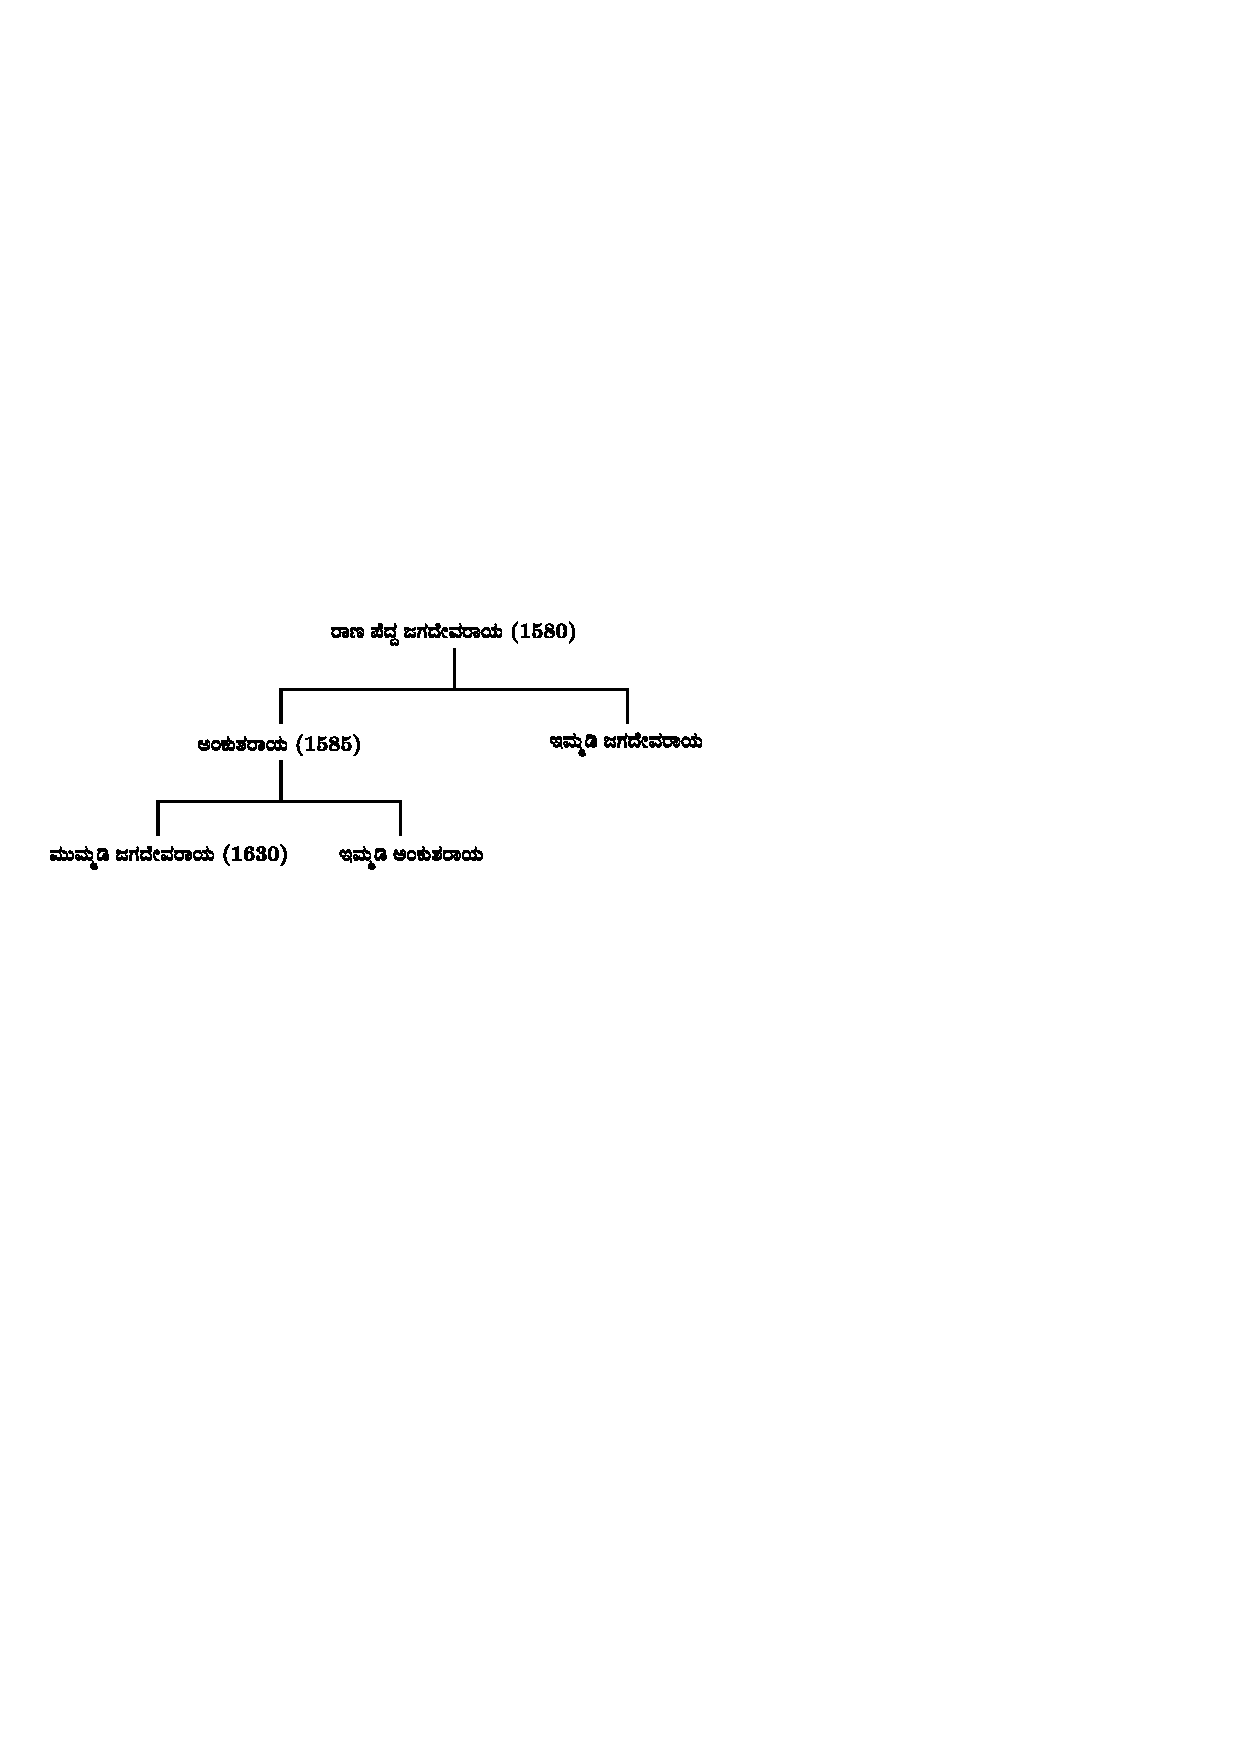
\includegraphics[scale=0.23]{"images/10.jpg"}
\caption{ಪ್ರಧಾನಮಂತ್ರಿ ನೆಹರು ಮತ್ತು ಸಿ. ವಿ. ರಾಮನ್, ಕರ್ನಾಟಕದ ಮುಖ್ಯಮಂತ್ರಿ ಹನುಮಂತಯ್ಯ (ಮದ್ಯ) ಕೇಂದ್ರದಲ್ಲಿದ್ದಾರೆ. \enginline{1957}ರಲ್ಲಿ ಬೆಂಗಳೂರಿನ ರೆಸಿಡೆನ್ಸಿಯಲ್ಲಿ ತೆಗೆದ ಚಿತ್ರ.}\label{chap3-fig01}
\end{figure}

\newpage

\heading{ಮಿರ್ಜಾ ಎಂ. ಇಸ್ಮಾಯಿಲ್}

ರಾಮನ್‍ರವರಿಗೆ ಅನೇಕ ಮಂದಿ ಅಭಿಮಾನಿಗಳಿದ್ದರು. ಕೆಲವರು ಶತ್ರುಗಳೂ ಮತ್ತು ಅವರ ಒಡನಾಟದ ಗಾಢ ಸ್ನೇಹಿತರೂ ಇದ್ದರು. ಸರ್ ಮಿರ್ಜಾ ಅವರು ಒಳ್ಳೆಯ ಸ್ನೇಹಿತರಾಗಿ ರಾಮನ್‍ರವರಿಗೆ ಅನೇಕ ಬಾರಿ ಸಹಾಯ ಮಾಡಿದರು. ರಾಮನ್ ಅವರಿಗೂ, ಮಿರ್ಜಾ ಅವರ ಹವ್ಯಾಸಗಳೂ, ಸಾಮರ್ಥ್ಯಗಳೂ ಮೆಚ್ಚುಗೆಯಾಗಿದ್ದವು. ಅವರು ರಾಮನ್ ಇನ್ಸ್ಟಿಟಿಟ್ಯೂಟ್‍ಗೆ ಬಂದದ್ದು ಒಂದೇ ಬಾರಿಯಾದರೂ, ಅದು ರಾಮನ್‍ರವರಿಗೆ ಅವಿಸ್ಮರಣೀಯವೆನಿಸಿತ್ತು.

ಭಾರತೀಯ ವಿಜ್ಞಾನ ಸಂಸ್ಥೆಯಲ್ಲಿ ರಾಮನ್‍ರವರಿಗೆ ಸಂಕಷ್ಟಗಳು ಎದುರಾದಾಗ ಮಿರ್ಜಾ ಅವರು ಮೈಸೂರಿನ ದಿವಾನರಾಗಿದ್ದರು. ಇನ್ಸ್ಟಿಟ್ಯೂಟ್‍ನಿಂದ ರಾಮನ್ ಅವರನ್ನು ಹೊರಹಾಕಲು ಹುನ್ನಾರ ನಡೆದಿತ್ತು. ಕೆಲವು ಪ್ರಭಾವಿ ವ್ಯಕ್ತಿಗಳಿಂದ ಇದು ತಪ್ಪಿತು. ಒಂದು ದಂತಕಥೆಯ ಪ್ರಕಾರ ಮಿರ್ಜಾ ಅವರು ಮಹಾರಾಜರ ಕಡೆಯಿಂದ ಆಗಿನ, ವೈಸ್‍ರಾಯ್ ಅವರಿಗೆ ಪ್ರಭಾವ ಬೀರಿ ಇದನ್ನು ತಪ್ಪಿಸಿದರು. ಹಾಗಾಗಿ ರಾಮನ್‍ರವರು ಭೌತಶಾಸ್ತ್ರ ವಿಭಾಗದ ಮುಖ್ಯಸ್ಥರಾಗಿ ಅದೇ ಸಂಸ್ಥೆಯಲ್ಲಿ ಮುಂದುವರಿಯುವ ಹಾಗಾಯಿತು.

ಮಿರ್ಜಾ ಅವರಿಗೆ ರಾಮನ್ ಅವರ ನೇರನುಡಿ ಇಷ್ಟವಾಗಿತ್ತು ಮತ್ತು ಅವರನ್ನು ನೈಜ ವಿಜ್ಞಾನಿಯಂತೆ ಮತ್ತು ಅತಿ ವರ್ಣರಂಜಿತ ವ್ಯಕ್ತಿಯಂತೆ ನೋಡಿದರು. ಮಿರ್ಜಾ ಅವರೂ, ರಾಮನ್ ನಂತೆಯೇ ಧೃಡ ಸಂಕಲ್ಪದ ದಿಟ್ಟ ವ್ಯಕ್ತಿ. ಅವರ ಪ್ರಕೃತಿ ಪ್ರೀತಿ ಹಾಗೂ ಸೌಂದರ್ಯ ಪ್ರಜ್ಞೆಗೆ ಹೆಸರು\- ವಾಸಿಯಾಗಿದ್ದರು. ಇಂದು ಉದ್ಯಾನ ನಗರಗಳೆನಿಸುವ  ಮೈಸೂರು ಮತ್ತು ಬೆಂಗಳೂರುಗಳನ್ನು ಬೆಳಸುವಲ್ಲಿ ಪ್ರಮುಖ ಪಾತ್ರವಹಿಸಿದ್ದರು. ಕರ್ನಾಟಕದ ಈ ನಗರಗಳಲ್ಲಿರುವ ಭವ್ಯ ಬಂಗಲೆಗಳು, ಸುಂದರ ಉದ್ಯಾನಗಳು ಮತ್ತು ಪಟ್ಟಣದ ವಿನ್ಯಾಸಗಳನ್ನು ಯಾರೇ ಆಗಲಿ ಗಮನಿಸದಿರರು.

ಮಿರ್ಜಾ ಇಸ್ಮಾಯಿಲ್ ಅವರಿಗೆ ಒಳ್ಳೆಯ ಅಭಿರುಚಿಗಳೂ ಮತ್ತು ರಾಜಗಾಂಭೀರ್ಯವೂ ಇದ್ದಿತು. ರಾಮನ್‍ರವರಿಗೆ ಇದಕ್ಕೆ ಸರಿಸಮನಾದ ವರ್ಣರಂಜಿತ ವ್ಯಕ್ತಿತ್ವವಿತ್ತು. ಇಬ್ಬರ ನಡುವಿನ ಸ್ನೇಹವು ಸ್ವಾಭಾವಿಕವಾಗಿತ್ತು ಮತ್ತು ಜೀವನಾದ್ಯಂತ ಮುಂದುವರಿದದ್ದು ನಿಜವೇ. \enginline{1934}ರಲ್ಲಿ ಇಂಡಿಯನ್ ಅಕಾಡೆಮಿ ಆಫ಼್ ಸೈನ್ಸ್‌ನ ಸಮ್ಮೇಳನವನ್ನು ಉದ್ಘಾಟಿಸಿದ್ದೊಂದೇ ಮಿರ್ಜಾರವರ ವೈಜ್ಞಾನಿಕ ಕಾರ್ಯವಾಗಿತ್ತು.


\heading{ಯಹುದಿ ಮೆನುಹಿನ್}

ಭಾರತೀಯ ಸಂಗೀತವನ್ನು ಅದಮ್ಯವಾಗಿ ಪ್ರೀತಿಸುತ್ತಿದ್ದ ಪ್ರಸಿದ್ಧ ವಯಲಿನ್ ವಾದಕರು ಯಹುದಿ ಮೆನುಹಿನ್. ಐನ್‍ಸ್ಟೈನ್‍ರವರಿಂದಲೇ ಜೀನಿಯಸ್ ಎಂದು ಕರೆಸಿಕೊಂಡ ಅವರು ಬಾಲ ಪ್ರತಿಭಾಶಾಲಿಯಾಗಿದ್ದರು.

ಬೆಂಗಳೂರಿಗೆ ಬಂದಿದ್ದಾಗ ಮೆನುಹಿನ್, ರಾಮನ್ ಅವರನ್ನು ಭೇಟಿಯಾದರು. ನನಗೆ ಈ ಭೇಟಿಯು ನೆನಪಿರುವುದೇಕೆಂದರೆ, ರಾಮನ್‍ರವರು ತಮ್ಮ ಕಛೇರಿಯಲ್ಲಿಟ್ಟಿದ್ದ ಪಿಟೀಲನ್ನು ಚೆನ್ನಾಗಿ ಒರೆಸಿಡಬೇಕೆಂದು ಹೇಳಿದ್ದರು. ಅಕಸ್ಮಾತ್ತಾಗಿ ಮೆನುಹಿನ್ ನುಡಿಸಬೇಕೆಂದಿದ್ದರೆ, ಅದು ಸಿದ್ಧವಾಗಿರಬೇಕಾಗಿತ್ತು.

ಮೆನುಹಿನ್ ಬಂದಾಗ, ರಾಮನ್‍ರವರು ತಮ್ಮ ಸಂಸ್ಥೆಯನ್ನು ತೋರಿಸಿದರು. ಅವರಿಗೆ ರಾಮನ್‍ರವರು ಪಿಟೀಲಿನ ಬಗ್ಗೆ ಮಾಡಿದ ಸಂಶೋಧನೆಯ ಅರಿವಿತ್ತು. ಇಬ್ಬರೂ ಈ ವಿಷಯದ ಬಗ್ಗೆ ಮಾತನಾಡಿದರು. ರಾಮನ್‍ರವರು, ಮೆನುಹಿನ್ ಇಚ್ಛಿಸಿದರೆ ಸಿದ್ಧವಾದ ಪಿಟೀಲನ್ನು\break ನುಡಿಸಬಹುದೆಂದು ಸೂಚಿಸಿದರು. ಆದರೆ ಮೆನುಹಿನ್ ಅವರು ಇದನ್ನು ಬಯಸದೆ, ನಯವಾಗಿ ಮಾತು ತಿರುಗಿಸಿದರು. ಏನಾದರೂ ಇದೊಂದು ಸ್ಮರಣೆಯ ಭೇಟಿಯಾಗಿತ್ತು. ಈ ಭೇಟಿಯನ್ನು ರಾಮನ್ ಬಹಳ ಇಷ್ಟ ಪಟ್ಟಿದ್ದರು.


\heading{ಜಿ. ಡಿ. ನಾಯ್ಡು}

ಕೊಯಮತ್ತೂರಿನ ಈ ಉದ್ಯಮಿ ರಾಮನ್ ಅವರ ಅಭಿಮಾನಿಯಾಗಿದ್ದರು. ಅವರ\break ಗೌರವವಾದರಗಳು ಪರಸ್ಪರವಾಗಿದ್ದವು. ನಾಯ್ಡು ಅವರು ಪ್ರತಿಭಾಶಾಲಿ. ಅವರು ಇಂಜಿನಿಯರಿಂಗ್ ಪದವಿ ಪಡೆಯದಿದ್ದರೂ ಯಂತ್ರ ವಿನ್ಯಾಸ ಚತುರರು. ಅವರಿಗೆ ಜರ್ಮನಿ ಮತ್ತು ಜರ್ಮನ್ ವಸ್ತುಗಳ ಬಗ್ಗೆ ವಿಪರೀತ ಆಸಕ್ತಿ ಇತ್ತು. ಅವರು ಅನೇಕ ಬಾರಿ ಜರ್ಮನಿಗೆ ಭೇಟಿಯಿತ್ತಿದ್ದರು. ಜನರು ಹೇಳುವಂತೆ ಅಲ್ಲಿನ ಉದ್ಯಮಿಗಳು, ನಾಯ್ಡುರವರು ಸೂಚಿಸಿದ ತೀಕ್ಷ್ಣ ಬುದ್ಧಿಯ ಉಜ್ವಲ ಸಲಹೆಗಳನ್ನು ತಮ್ಮ ಕಾರ್ಖಾನೆಗಳ ಯಂತ್ರಗಳಲ್ಲಿ ಮಾರ್ಪಾಡು ಮಾಡಿಕೊಂಡರು. ನಾಯ್ಡು ಅವರು ಬಹಳ ಬುದ್ಧಿವಂತರು. ಅವರು ಸ್ವಯಂ ವಿದ್ಯಾಪಾರಂಗತರು. ಅವರು ತಮ್ಮ ಹಠಮಾರಿತನಕ್ಕೂ, ವಿಲಕ್ಷಣ ವ್ಯಕ್ತಿತ್ವಕ್ಕೂ ಹೆಸರಾಗಿದ್ದರು. ಅವರು ತಮಾಷೆಗಾಗಿ ಇತರರನ್ನು ಇಕ್ಕಟ್ಟಿಗೆ ಸಿಲುಕಿಸುವುದರಲ್ಲಿ ನಿಷ್ಣಾತರು. ಅದರಲ್ಲೂ ಆದಾಯ ತೆರಿಗೆ ಅಧಿಕಾರಿಗಳನ್ನು ಮುಖ್ಯವಾಗಿ ಗುರಿಮಾಡುತ್ತಿದ್ದರು. ಜೀವನದುದ್ದಕ್ಕೂ ಸಾಣೆ ಹಿಡಿಸಬೇಕಾಗಿಲ್ಲದ ಬ್ಲೇಡನ್ನು ಮಾಡಿದರು. ಅದನ್ನು ಪರೀಕ್ಷಿಸಲು ಎಲ್ಲರಿಗೂ ಕೊಡುತ್ತಿದ್ದರು. ರಾಮನ್‍ರವರಿಗೆ ನೀಡಿದ ಇಂತಹ ಬ್ಲೇಡುಗಳನ್ನು ಇನ್ಸ್ಟಿಟ್ಯೂಟ್‍ನಲ್ಲಿ ನಾನು ನೋಡಿದ್ದೇನೆ. ಅವರು ಹೇಳಿದಂತೆ ಈ ಬ್ಲೇಡುಗಳು ಇದ್ದವಾದರೂ, ಅವು ವಾಣಿಜ್ಯ ರಂಗದಲ್ಲಿ ಗೆಲ್ಲಲಾಗಲಿಲ್ಲ. ಸಸ್ಯಗಳ ಕಸಿಯಲ್ಲೂ ಅವರದ್ದು ಎತ್ತಿದ ಕೈ. ಒಂದು ವಿಧದ ಪಪ್ಪಾಯಿಯನ್ನು ಕಸಿಮಾಡಿ ಬೆಳಸಿದ್ದರು. ಅದು ಅತಿಹೆಚ್ಚು ಸಿಹಿಯಾಗಿಯೂ, ಅತಿ ದೊಡ್ಡ ಗಾತ್ರಕ್ಕೂ ಇರುವ ಕಾಯಿ ಬಿಡುತ್ತಿತ್ತು. ರಾಮನ್ ಮತ್ತು ನಾಯ್ಡು ಅವರು ಪರಸ್ಪರ ಅಭಿಮಾನಿಗಳಾಗಿದ್ದರು. ಕೊಯಮತ್ತೂರಿಗೆ ಭೇಟಿಯಿತ್ತಾಗಲೆಲ್ಲಾ ರಾಮನ್, ನಾಯ್ಡು ಅವರೊಡನೆ ಕಾಲ ಕಳೆಯುತ್ತಿದ್ದರು. ನಾಯ್ಡು ಅವರು ಒಮ್ಮೆ ಮಾತ್ರ ರಾಮನ್ ಇನ್ಸ್ಟಿಟ್ಯೂಟ್‍ಗೆ ಬಂದಿದ್ದರು, ಅಂದು ರಾಮನ್ ತಮ್ಮ ಸಂಗ್ರಹವನ್ನು ಅಭಿಮಾನದಿಂದ ತೋರಿಸಿದ್ದರು.

ನಾಯ್ಡು ಅವರು, ರಾಮನ್‍ರವರಿಗೆ ಸ್ಟೀಲ್ ವೈರ್ ರೆಕಾರ್ಡ್ ರನ್ನು ಉಡುಗೊರೆಯಾಗಿತ್ತರು. ಇದು ಆಧುನಿಕ ಟೇಪ್ ರೆಕಾರ್ಡ್‌ನ ಹಿಂದಿನ ಅವತಾರವಾಗಿತ್ತು. ಈ ಯಂತ್ರ ಚೆನ್ನಾಗಿ ಕೆಲಸ ಮಾಡುತ್ತಿತ್ತು. ಇದನ್ನು \enginline{1952}ರ ವಿಜ್ಞಾನ ಸಮ್ಮೇಳನದಲ್ಲಿ ರಾಮನ್ ಅವರ ಭಾಷಣವನ್ನು ರೆಕಾರ್ಡ್ ಮಾಡಲು ಬಳಸಿದ್ದೆ. ಭಾಷಣವು ಜಾಲಕ ಗತಿಶೀಲತೆಯ ವಿಷಯವಾಗಿತ್ತು. ಅಂದು ಸಮ್ಮೇಳನಕ್ಕೆ ಬಂದಿದ್ದ ಪ್ರತಿಷ್ಠಿತ ವಿಜ್ಞಾನಿಗಳಾದ ರುಡೋಲ್ಭ್ ಪೈಲ್ಸ್ ಮತ್ತು ಜಿ. ವೆಂಟಸೆಲ್ ಅವರು ಬಹುದೊಡ್ಡ ಸಭಿಕರ ಗುಂಪಿನಲ್ಲಿದ್ದರು.


\heading{ಪಂಡಿತ್ ಜವಾಹರಲಾಲ್ ನೆಹರು}

ಪ್ರಧಾನ ಮಂತ್ರಿ ನೆಹರೂ ಅವರು ಬಂದದ್ದು ನಮಗೆಲ್ಲಾ ಅವಿಸ್ಮರಣೀಯವಾಗಿತ್ತು. ಅವರು ತಮ್ಮ ಇಬ್ಬರು ಮೊಮ್ಮಕ್ಕಳು ಮತ್ತು ಮಗಳು ಇಂದಿರಾ ಅವರೊಂದಿಗೆ ಬೆಂಗಳೂರಿಗೆ ಬಂದಿದ್ದರು. ಶ‍್ರೀಮತಿ ಗಾಂಧಿಯವರು ಬಂದಾಗ, ರಾಮನ್ ತಮ್ಮ ಸಂಸ್ಥೆಯ ಯಾತ್ರೆ ಮಾಡಿಸಿದರು. ಇಂದಿರಾ ಅವರು ಆಗ ಸುಮಾರು \enginline{40} ವಯಸ್ಸಿನವರಿದ್ದಿರಬಹುದು. ಸೀರೆ ಧರಿಸಿ ಬಹಳ ಅಂದವಾಗಿಯೂ, ಆಕರ್ಷಕವಾಗಿಯೂ ಕಾಣುತ್ತಿದ್ದರು. ರಾಮನ್‍ರವರು ಸ್ಫಟಿಕಗಳ ಅಂದವನ್ನು ವಿವರಿಸುವಾಗ ಒಳ್ಳೆಯ ಹುರುಪಿನಲ್ಲಿದ್ದರು. ಅವರು ಪ್ರತಿದೀಪ್ತಿಯಾಗುವ ಖನಿಜಗಳನ್ನೂ, ರತ್ನಗಳನ್ನೂ ತೋರಿಸಿದರು. ಸಂಗ್ರಹಾಲಯಗಳನ್ನು ತೋರಿಸಿದ ಬಳಿಕ ಶ‍್ರೀಮತಿ ಗಾಂಧಿಯವರನ್ನು ಮಹಡಿಯ ಮೇಲೆ ಕರೆದೊಯ್ದರು. ದೂರದ ನಂದಿ ಬೆಟ್ಟವನ್ನೂ ಸುಂದರ ದಿಗಂತವನ್ನೂ ತೋರಿಸಿದರು. ಹೊರಡುವಾಗ “ನೀವು ತುಂಬ ದಣಿದಿರಬಹುದು. ಕಟ್ಟಡದ ಮೇಲೆ ಕೆಳಗೆ ಓಡಾಡಿದ್ದೀರಿ. ನೀವು ರೆಸಿಡೆನ್ಸಿಗೆ ತೆರಳಿ ವಿರಮಿಸುವುದು ಒಳ್ಳೆಯದು”. ಅನಂತರ ಯೋಚಿಸಿ “ನಿಮ್ಮ ತಂದೆಯವರಿಗೆ ನೀವು ನೋಡಿದ್ದನ್ನು ಹೇಳಿ ಅವರನ್ನು ನಮ್ಮ ಸಂಸ್ಥೆಗೆ ಬರುವಂತೆ ಮಾಡಿ” ಎಂದರು.

ಅದೇ ದಿನ ಮಧ್ಯಾಹ್ನ ಪ್ರಧಾನ ಮಂತ್ರಿಗಳ ಕಾರ್ಯದರ್ಶಿಗಳು ರಾಮನ್‍ರವರಿಗೆ ಫೋನ್ ಮಾಡಿ, ಅನುಕೂಲವಿದ್ದರೆ ಮಾರನೇ ದಿನ ಪ್ರಧಾನ ಮಂತ್ರಿಗಳು ಭೇಟಿಗೆ ಬರುತ್ತಾರೆಂದು ತಿಳಿಸಿದರು. ರಾಮನ್‍ರವರು ಉತ್ಸಾಹದಿಂದ ಮನವಿಯನ್ನು ಅಂಗೀಕರಿಸಿದರು ಮತ್ತು ತಯಾರಿ ಶುರು ಮಾಡಿದರು. ನಿಗದಿತ ಸಮಯದಲ್ಲಿ ಕಂದು ಬಣ್ಣದ ಉದ್ದನೆಯ ಕೋಟು ಮತ್ತು ಬಿಳಿಯ ಅಚ್‍ಕನ್ ತೊಟ್ಟು ಪ್ರಧಾನ ಮಂತ್ರಿಗಳು ತಮ್ಮ ಪರಿವಾರದೊಡನೆ ಆಗಮಿಸಿದರು. ರಾಮನ್‍ರವರು ಹಸ್ತಲಾಘವ ಕೊಟ್ಟು ಆದರದಿಂದ ಬರಮಾಡಿಕೊಂಡರು. ನನ್ನ ಎಂಟು ವರ್ಷದ ಮಗಳು ಗೀತಾ, ನೆಹರೂ ಅವರಿಗೆ ಗುಲಾಬಿ ಹೂಗುಚ್ಛವೊಂದನ್ನು ನೀಡಿದಳು. ನೆಹರೂ ಅವರ ಮುಖ ಅಗಲವಾಯಿತು. ರಾಮನ್‍ರವರು ಸಹ ಒಂದು ಸುಂದರ ಗುಲಾಬಿ ಹೂವನ್ನು ನೀಡಿದರು. ಇದನ್ನು ನೆಹರೂ ಅವರು ತಮ್ಮ ಕೋಟಿಗೆ ಸಿಕ್ಕಿಸಿಕೊಂಡರು. ಕೋಟಿನ ಬಟನ್ ರಂದ್ರದಲ್ಲಿ ಹೂ ಇಟ್ಟುಕೊಳ್ಳುವುದೆಂದರೆ ನೆಹರೂರವರಿಗೆ ಬಹಳ ಇಷ್ಟ. ನೆಹರೂ ಅವರು ಅಚ್ಚುಕಟ್ಟಾಗಿ ಮಾತನಾಡಿ ಬಹಳ ಆಪ್ಯಾಯಮಾನ\-ವಾಗಿ ವರ್ತಿಸಿದರು. ರಾಮನ್ ಮತ್ತು ಅವರ ಶ್ರಿಮತಿಯವರ ಬಗ್ಗೆ ವಿಚಾರಿಸಿಕೊಂಡರು. ಇದಾದನಂತರ ಇಡೀ ತಂಡವನ್ನು ರಾಮನ್, ತಮ್ಮ ಸಂಗ್ರಹಾಲಯ, ಗ್ರಂಥಾಲಯ ಮತ್ತು ಉಪನ್ಯಾಸ ಕೊಠಡಿಗಳಿಗೆ ಕರೆದೊಯ್ದರು. ಗ್ರಂಥಾಲಯದಲ್ಲಿ ರಾಮನ್‍ರವರು ಸಿಬ್ಬಂದಿಯನ್ನು ನೆಹರೂ ಅವರಿಗೆ ಪರಿಚಯಿಸಿದರು. ನೆಹರು ಆತ್ಮೀಯತೆಯಿಂದ ನಮಗೆ ಹಸ್ತಲಾಘವ ಕೊಟ್ಟರು.

ಉಪನ್ಯಾಸ ಕೊಠಡಿಯಲ್ಲಿ ಹದಿನೈದು ನಿಮಿಷಗಳ ಕಾಲ ರಾಮನ್‍ರವರು ತಮ್ಮ ಸಂಸ್ಥೆಯ ಭವಿಷ್ಯಕ್ಕೆ ಒಂದು ನಿಧಿ ಸ್ಥಾಪನೆ ಅಗತ್ಯವೆಂದು ತಿಳಿಸಿ, ಅದಕ್ಕೆ ಸರ್ಕಾರದವರು ಹತ್ತು ಲಕ್ಷ ರೂಪಾಯಿಯ ದತ್ತಿ ಸ್ಥಾಪಿಸಬಹುದೆಂದು ಮನವಿ ಮಾಡಿದರು. ಮಾತು ಮುಗಿದ ನಂತರ ನೆಹರೂ ಎದ್ದು ನಿಂತು ರಾಮನ್ ಅವರ ಕಡೆ ತಿರುಗಿ \enginline{-} “ರಾಮನ್ ಅವರೇ ನಿಮ್ಮ ಸಂಸ್ಥೆಯ ಬಗ್ಗೆ ನೀವೇಕೆ ಚಿಂತಿಸುವಿರಿ? ಸರ್ಕಾರವು ಸಂತೋಷದಿಂದ ಅದನ್ನು ನೋಡಿಕೊಳ್ಳುತ್ತದೆ” ಎಂದರು. ಇದಕ್ಕೆ ರಾಮನ್‍ರವರು\enginline{--}\break “ಸರ್, ರಾಜಕಾರಣಿಗಳ ಭವಿಷ್ಯವನ್ನು ಮತ್ತು ಅವರ ನುಡಿಗಳನ್ನೂ ಯಾರು ತಾನೇ ಬಲ್ಲರು? ನನಗೆ ನಿಮ್ಮಂದ ಅನಿರ್ಬಂಧಿತ ವಾಗ್ದಾನ ಬೇಕಿದೆ. ಇದೊಂದು ಸರ್ಕಾರಿ ಪ್ರಯೋಗಾಲಯವಾಗಲು ನನಗೆ ಇಷ್ಟವಿಲ್ಲ” ಎಂದರು. ನೆಹರು ಮುಗುಳ್ನಕ್ಕು ಮುಂದೆ ಸಾಗಿದರು. ಪ್ರತಿಕ್ರಿಯಿಸಲಿಲ್ಲ. ಉಳಿದಂತೆ ಭೇಟಿಯು ಸುಗಮವಾಗಿತ್ತು ಮತ್ತು ನಗುನಗುತ್ತಾ ಈರ್ವರೂ ಬೀಳ್ಕೊಂಡರು.

ಅಂದು ಅಲ್ಲೇ ಒಂದು ತೀರ್ಮಾನಕ್ಕೆ ಬರಬಹುದೆಂಬ ರಾಮನ್‍ರವರಿಗೆ ನಿರಾಸೆಯಾಯಿತು. ಅವರಿಗೆ, ಪ್ರಧಾನ ಮಂತ್ರಿಗಳೂ ಸಹ ಆತುರದಲ್ಲಿ ಈ ವಿಷಯದ ಬಗ್ಗೆ ನಿರ್ಧರಿಸಲಾರರೆಂದು ತಿಳಿದಿತ್ತು. ಏಕೆಂದರೆ ಅವರು ಪಾರ್ಲಿಮೆಂಟಿಗೆ ಅಧೀನರಾಗಿದ್ದರು. ರಾಮನ್ ತಮ್ಮ ಮಾತುಗಳು ಕಟುವಾಗಿದ್ದುವೆ ಎಂದು ನನಗೆ ಕೇಳಿದರು ನಾನು ಹೌದು ಎಂದೆ. ಆದರೆ ನೆಹರು ಅವರು ಇದನ್ನು ತೋರಿಸಿಕೊಳ್ಳಲಿಲ್ಲ. ಬಹಳ ದಿನಗಳಾದ ಮೇಲೆ ತಾವು ಯಾರಿಗೂ, ಅಂದರೆ ಪ್ರಧಾನ ಮಂತ್ರಿಗಳಿಗೂ ಭಯ ಪಡುವುದಿಲ್ಲವೆಂದು ಹೇಳಿದರು. ಅವರು ತಮಗೆ ಸರಿ ಎನಿಸಿದ್ದನ್ನು ನೂರು ಶತ ಹೇಳಿದ್ದಾರೆ ಎಂದರು. ರಾಮನ್‍ರವರು ನಿರ್ಭಯರಾಗಿದ್ದರು. ಅವರಿಗೆ ಹೃದಯಕ್ಕೆ ತಟ್ಟಿದ್ದನ್ನು ಹೇಳಲು ಅವರಿಗೆ ಯಾವ ಮುಜುಗರವೂ ಇರಲಿಲ್ಲ. ಈ ಗುಣವನ್ನು ಅವರು ಕೊನೆಯವರೆಗೂ ಮೀರಲಾಗಲಿಲ್ಲ. ಇದೊಂದರಿಂದಲೇ ಅವರಿಗೆ ಎಲ್ಲ ಸಮಸ್ಯೆಗಳೂ ಉಂಟಾದವು.

ನೆಹರೂ ಅವರು ತಮ್ಮ ಭೇಟಿಯ ಬಗ್ಗೆ, ತಮಗುಂಟಾದ ಸಂತೋಷದ ಬಗ್ಗೆ ರಾಮನ್‍ರವರಿಗೆ ಪತ್ರ ಬರೆದು ಶ್ಲಾಘಿಸಿದರು.


\heading{ಶ‍್ರೀ ಪ್ರಕಾಶ}

ಉತ್ತರ ಪ್ರದೇಶದ ಪ್ರಕಾಂಡ ಪಂಡಿತರ ಕುಟುಂಬದಿಂದ ಬಂದವರು, ಬಹಳ ಕಾಲ ಮದರಾಸಿನ ಗೌರ್ನರ್ ಆಗಿದ್ದ ಶ‍್ರೀ ಪ್ರಕಾಶ ಅವರು ಭಗವಾನ್ ದಾಸ್ ಅವರ ಪುತ್ರರು. ಭಗವಾನ್~~ದಾಸ್ ಅವರೂ ಪಂಡಿತರಾಗಿದ್ದು ‘ಭಾರತ ರತ್ನ’ ಪ್ರಶಸ್ತಿಗೆ ಭಾಜನರಾಗಿದ್ದರು. ಭಾರತ ದೇಶದಲ್ಲಿ ಕೊಡಮಾಡುವ ಅತಿಶ್ರೇಷ್ಠ ಪ್ರಶಸ್ತಿ ಇದಾಗಿದೆ.

ಬೆಂಗಳೂರಿಗೆ ಬಂದಾಗ ಶ‍್ರೀ ಪ್ರಕಾಶ ಅವರು ರಾಮನ್ ಅವರನ್ನು ನೋಡಲು ಬಂದರು. ರಾಮನ್ ಸಂಸ್ಥೆಯು ಆಗ ತಾನೆ ಶುರುವಾಗಿದ್ದು, ಕಟ್ಟಡವು ಪೂರ್ಣವಾಗಿರಲಿಲ್ಲ. ನೀರು ಇತ್ಯಾದಿಗಳಿಗೆ ಇನ್ನೂ ವ್ಯವಸ್ಥೆ ಇರಲಿಲ್ಲ. ಗವರ್ನರ ಸಿಬ್ಬಂದಿಯು ಬಾಜಾಭಜಂತ್ರಿಗಳೊಡನೆ ಬಂದಿತು. ರಾಮನ್ ಬಹಳ ಗೌರವದಿಂದ ಅವರನ್ನು ಬರಮಾಡಿಕೊಂಡರು.

ಸಂಗ್ರಹಾಲಯಗಳನ್ನು ತೋರಿಸಿಯಾದ ಮೇಲೆ ರಾಮನ್‍ರವರು ತಮ್ಮ ನೆನಪಿನ ಕಾಣಿಕೆಗಳನ್ನು ಪ್ರದರ್ಶಿಸಬೇಕೆಂದಿದ್ದರು. ಆಗ ಶ‍್ರೀ ಪ್ರಕಾಶ ಅವರು ಶೌಚಾಲಯ ಎಲ್ಲಿದೆ ಎಂದು ಕೇಳಿದರು. ರಾಮನ್‍ರವರು ತಮ್ಮ ಕಛೇರಿಯ ಪಕ್ಕದಲ್ಲಿದ್ದ ಖಾಸಗಿ ಶೌಚಾಲಯ ಅನ್ನು ತೋರಿಸಿದರು.\break ಶೌಚಾಲಯ ಬಳಸಿದ ನಂತರ ಗವರ್ನರ್‌ರವರು ಅಲ್ಲಿ ನೀರು ಇಲ್ಲವೆಂಬುದನ್ನು ಕಂಡುಕೊಂಡರು. ಅಲ್ಲಿ ಟಿಶ್ಯೂ ಪೇಪರೂ ಇರಲಿಲ್ಲ. ಬೆಂಗಳೂರು ಜಲ ಮಂಡಳಿಯೂ ಅಂದಿಗೂ ಸಮರ್ಪಕ ನೀರು ಸರಬರಾಜು ಮಾಡುತ್ತಿರಲಿಲ್ಲ. \enginline{40} ವರ್ಷಗಳಾದ ಬಳಿಕವೂ ಸುದಾರಿಸಿಲ್ಲ, ಸಂಸ್ಥೆಗೆ ನೀರಿನ ಸರಬರಾಜಿಗೆ ನೀರು ಶೇಖರಣೆಗೆ ಟ್ಯಾಂಕ್ ಒಂದನ್ನು ನಿರ್ಮಿಸಲಾಗುತ್ತಿತ್ತು. ಗೌರ್ನರ್ ಸಾಹೇಬರು ನೀರು ಕೊಡಿ ಎಂದು ಆರ್ತನಾದ ಮಾಡತೊಡಗಿದರು. ಅದೃಷ್ಟವಶಾತ್ ರಾಮನ್ ತಮ್ಮ ಕಛೇರಿಯಲ್ಲಿದ್ದರು. ಗವರ್ನರ್‌ರ ಕೂಗನ್ನು ಕೇಳಿಸಿಕೊಂಡರು. ಅವರೂ ಸಹ ಸಹಾಯಕ್ಕಾಗಿ ಕೂಗಿಕೊಂಡರು. ಗವರ್ನರ್‌ರ ಎ.ಡಿ.ಸಿ. ಏನೂ ತೋಚದೆ ಅತ್ತಿತ್ತ ಓಡುತ್ತಿದ್ದರು. ಅವರಿಗೆ ಕಟ್ಟಡವೇ ಹೊಸದು. ರಾಮನ್‍ರವರಿಗೆ ಒಂದು ಉಪಾಯ ಹೊಳೆಯಿತು. ತಮ್ಮ ಕಛೇರಿಯಲ್ಲಿದ್ದ ಕುಡಿಯುವ ನೀರಿನ ಮಣ್ಣಿನ ಹೂಜಿಯನ್ನು ಟಾಯ್ಲೆಟ್ ನ ಬಾಗಿಲಲ್ಲಿ ಇಟ್ಟು, “ರೀ, ಶ‍್ರೀ ಪ್ರಕಾಶ ಅವರೇ, ಬಾಗಿಲಲ್ಲಿ ನೀರಿನ ಮಡಕೆ ಇಟ್ಟಿದ್ದೇನೆ. ಇದನ್ನೇ ಹೇಗೆ ಬೇಕಾದರೂ ಬಳಸಿಕೊಳ್ಳಿ” ಎಂದರು. ಗವರ್ನರ್‌ರು ಅದನ್ನೇ ಒಳಗೆ ಎಳೆದುಕೊಂಡು ಕೊಂಚ ಕಾಲದ ನಂತರ ನಗುತ್ತಾ ಹೊರಬಂದರು. ರಾಮನ್ ಏನೂ ಆಗದವರಂತೆ ತಮ್ಮ ಪೂರ್ವಯೋಜಿತ ಕಾರ್ಯದಲ್ಲಿ ಮಗ್ನರಾದರು. ಗವರ್ನರರಿಗೆ ಭರ್ಜರಿ ಬೀಳ್ಕೊಡುಗೆಯೂ ಆಯಿತು.

ಇದಾದ ಬಳಿಕ ಕಟ್ಟಡದ ಕಂಟ್ರಾಕ್ಟರರಿಗೆ ಮೊದಲು ನೀರಿನ ಟ್ಯಾಂಕ್ ವ್ಯವಸ್ಥೆ ಪೂರ್ಣಗೊಳಿಸ\-ಬೇಕೆಂದು ತಾಕೀತು ಮಾಡಲಾಯಿತು.


\heading{ಸರ್. ಎಂ. ವಿಶ್ವೇಶ್ವರಯ್ಯ}

ಕರ್ನಾಟಕದ ಸುಪ್ರಸಿದ್ಧ ಇಂಜಿನಿಯರ್ ಎಂ.ವಿಶ್ವೇಶ್ವರಯ್ಯನವರು ಅಂದಿನ ಮೈಸೂರು\break ಸಂಸ್ಥಾನದಲ್ಲಿ ಅನೇಕ ಉದ್ಯಮಗಳನ್ನು ಸ್ಥಾಪಿಸುವುದಕ್ಕೆ ಕಾರಣರಾದವರು. ಭದ್ರಾವತಿಯ ಕಬ್ಬಿಣದ ಉದ್ಯಮವೂ ಮತ್ತು ಅನೇಕ ಜಲವಿದ್ಯುತ್ ಯೋಜನೆಗಳೂ ಇವರ ಕನಸಿನಿಂದ ಬಂದವು.

ಅವರ ತಮ್ಮ ದೂರದೃಷ್ಠಿಗೂ ಮತ್ತು ಕರ್ತೃತ್ವ ಶಕ್ತಿಗೂ ಹೆಸರಾಗಿದ್ದರು. ಅವರು ಸಂಸ್ಥಾನದ ದಿವಾನರಾಗಿ ಕೆಲಸಮಾಡಿದ್ದರು. ಅವರು ಶತಾಯುಷಿಯಾಗಿ, ಶಿಸ್ತು ಸಂಯಮಗಳನ್ನು ಕೊನೆಗಾಲದ\-ವರೆಗೂ ರೂಢಿಸಿಕೊಂಡರು. ಅವರು ಯಾವಾಗಲೂ ಜರಿಪೇಟ ಮತ್ತು ಭರ್ಜರಿ ಸೂಟ್‍ನಲ್ಲಿಯೇ ಕಾಣಿಸಿಕೊಳ್ಳುತ್ತಿದ್ದರು.

ರಾಮನ್ ಮತ್ತು ವಿಶ್ವೇಶ್ವರಯ್ಯನವರು ಪರಸ್ಪರ ಒಡನಾಡಿಗಳಾಗಿದ್ದಿರಬಹುದು. ಆದರೆ ನನ್ನ ಕಾಲದಲ್ಲಿ ಅವರು ರಾಮನ್ ಸಂಸ್ಥೆಯನ್ನು ನೋಡಲು ಒಮ್ಮೆ ಮಾತ್ರ ಬಂದಿದ್ದರು. ಅದೂ ಅವರ ಅತಿ ವೃದ್ಧಾಪ್ಯದಲ್ಲಿ. ಅವರು ತುಂಬ ನಿತ್ರಾಣರಾಗಿದ್ದರಿಂದ ಅವರನ್ನು ಇಬ್ಬರು ಹೊತ್ತು ತರಬೇಕಾಗಿತ್ತು, ಆಗಲೂ ಅವರು ಸೂಟುಧಾರಿಗಳಾಗಿದ್ದರು ಮತ್ತು ಅವರ ಬುದ್ಧಿಶಕ್ತಿಗಳು ಚುರುಕಾಗಿದ್ದವು. ರಾಮನ್ ಅವರನ್ನು ಆದರಿಸಿ ತಮ್ಮ ಸಂಸ್ಥೆಯ ಬಗ್ಗೆ ವಿವರಣೆ ನೀಡಿದರು. ವಿಶ್ವೇಶ್ವರಯ್ಯನವರು\enginline{--} “ರಾಮನ್ ನೀವು ಸಮಾಜದ ಒಳತಿಗಾಗಿಯೂ ಏನಾದರೂ ಮಾಡಬೇಕು ನಿಮ್ಮ ವೈಜ್ಞಾನಿಕ ಸಂಶೋಧನೆಯು ಜನರಿಗೆ ಉಪಯೋಗವಾಗುವಂತಿರಬೇಕು” ಎಂದು ಬಿಟ್ಟರು. ಇದು ರಾಮನ್‍ರವರಿಗೆ ಹಿಡಿಸಲಿಲ್ಲ. ಆದರೆ ಮೌನವಾಗಿದ್ದರು. ಅನಂತರ ರಾಮನ್ ನನಗೆ ಹೀಗೆ ಹೇಳಿದರು\enginline{--} “ಈ ಜರ್ಝರಿತ ಮುದುಕ ನನಗೆ ಇದನ್ನು ಹೇಳಲು ಇಷ್ಟು ದೂರ ಬರಬೇಕಿತ್ತೆ?”. ಈ ಭೇಟಿಯ ಕೊಂಚ ದಿನಗಳಲ್ಲೇ ವಿಶ್ವೇಶ್ವರಯ್ಯನವರು ಕಾಲವಾದರು. ಮೈಸೂರು ಸಂಸ್ಥಾನದ ಔದ್ಯಮೀಕರಣಕ್ಕೆ ಬಹಳಷ್ಟು ದುಡಿದ ಮುತ್ಸದ್ಧಿ ಕಣ್ಮರೆಯಾದರು.

\newpage

\heading{ಮೈಸೂರಿನ ಮಹಾರಾಜ ಜಯಚಾಮರಾಜೇಂದ್ರ ಒಡೆಯರ್}

ರಾಮನ್‍ರವರು ಮೈಸೂರಿನ ಮಹಾರಾಜರನ್ನು ವಿಶೇಷವಾಗಿ ಮೆಚ್ಚುತ್ತಿದ್ದರು. ರಾಮನ್ ಅವರ ಸಾಧನೆಗಳನ್ನು ಶ್ಲಾಘಿಸುತ್ತಿದ್ದ ಮಹಾರಾಜರು ಅವರಿಗೆ ಹಲವಾರು ಬಾರಿ ಬೆಂಬಲವಾಗಿ ನಿಂತಿದ್ದರು. ರಾಮನ್ ತಮ್ಮ ಕನಸಿನ ಇನ್ಸ್ಟಿಟ್ಯೂಟ್ ಮಾಡಲು ಅವರ ಸಹಾಯ ಕೋರಿದಾಗ, ಹನ್ನೊಂದು ಎಕರೆ ಭೂಮಿಯನ್ನು ಮಂಜೂರು ಮಾಡಿದರು. ಅಲ್ಲದೆ ಸಂಸ್ಥೆಯ ನಿರ್ದೇಶಕರಿಗೆ ನಿವಾಸ ಕಟ್ಟಲು ರಾಮನ್ ಮತ್ತೆ ಕೋರಿದಾಗ, ಪಕ್ಕದ ನಾಲ್ಕು ಎಕರೆ ಭೂಮಿಯನ್ನೂ ನೀಡಿದರು.

ರಾಮನ್‍ರವರಿಗೆ ಭೂ ಆಸ್ತಿಯ ಮೇಲಿನ ಹೂಡಿಕೆ ಕರಗತವಾಗಿತ್ತು ಮತ್ತು ಅದರಲ್ಲಿ ಯಾವಾಗಲೂ ಲಾಭಗಳಿಸುತ್ತಿದ್ದರು. ಒಮ್ಮೆ ಮದರಾಸಿನ ಆಳ್ವಾರ್ ಪೇಟೆಯಲ್ಲಿ ಹಲವಾರು ಎಕರೆ ಭೂಮಿಯನ್ನು ಕೊಂಡಿದ್ದರು. ಆಗ ಅಲ್ಲಿ ಭೂಮಿಯ ಬೆಲೆ ಕನಿಷ್ಠವಾಗಿತ್ತು. ಅದು ಅತಿ ಶೀಘ್ರವಾಗಿ ಸಾವಿರ ಪಟ್ಟು ಬೆಲೆಯಾಯಿತು. ಆಗಿನ ಕಾಲದಲ್ಲಿ ಸುಮಾರು ಹತ್ತು ಲಕ್ಷ ರೂಪಾಯಿಗಳ ಲಾಭಗಳಿಸಿ ತಮ್ಮ ಸಂಸ್ಥೆಗೆ ಉಪಯೋಗಿಸಿಕೊಂಡರು. ಮಹಾರಾಜರ ಭೂಮಿ ದೇಣಿಗೆಯು ರಾಮನ್‍ರವರಿಗೆ ಅತಿಮೌಲ್ಯದ ಮತ್ತು ಶ್ರೇಷ್ಠ ಉಡುಗೊರೆಯಾಗಿತ್ತು.

ಮಹಾರಾಜರು ರಾಮನ್‍ರವರಿಗೆ ಸಂಸ್ಥಾನದ ಸನ್ಮಾನ ನೀಡಿದ್ದರಿಂದ, ಅವರಿಗೆ ಅರಮನೆಯ ಅಧಿಕೃತ ದರ್ಬಾರ್ ನಲ್ಲಿ ಅವಕಾಶ ಮತ್ತು ಕರ್ತವ್ಯಗಳಿದ್ದವು. ದಸರಾ ದಿನಗಳಲ್ಲಿ ದರ್ಬಾರ್ ಕರೆದಾಗ ಅದಕ್ಕಾಗಿ ನಿಯೋಜಿಸಿದ್ದ ಉಡುಗೆಯನ್ನು ಧರಿಸಿ, ಮಹಾರಾಜರ ಮುಂದೆ ಗೌರವ ಸಲ್ಲಿಸಬೇಕಾಗಿತ್ತು. ರಾಮನ್‍ರವರಿಗೆ ನಿರಂತರವಾಗಿ ದರ್ಬಾರ್‍ಗೆ ಆಹ್ವಾನವಿರುತ್ತಿತ್ತು.

ಸ್ವಾತಂತ್ರ್ಯ ಬಂದ ನಂತರ ಸಂಸ್ಥಾನವು ಮಾಯವಾಗಿ ಕರ್ನಾಟಕ ರಾಜ್ಯವಾಯಿತು, ಜನಪ್ರಿಯ ಸರ್ಕಾರ ಬಂದಿತು, ಜಯಚಾಮರಾಜೇಂದ್ರರು ಮದರಾಸಿನ ಗೌರ್ನರ್ ಆದರು. ಅಲ್ಲಿ ಅವರು ಐದು ವರ್ಷಗಳ ಕಾಲ ಇದ್ದರು. ಈ ಅವಧಿಯಲ್ಲಿ ರಾಮನ್ ಸಂಸ್ಥೆಗೆ ಅವರು ಬಂದಿದ್ದರು. ರಾಮನ್‍ರವರು ಆದ್ಧೂರಿಯ ಸಮಾರಂಭವನ್ನು ಆಯೋಜಿಸಿದರು. ಅವರಿಗೆ ಭರ್ಜರಿ ಸ್ವಾಗತ ನೀಡಿದರು. ಮಹಾರಾಜರು ನೋಡಲು ಆಕರ್ಷಕ ವ್ಯಕ್ತಿ. ಅತಿ ಗಂಭೀರ ಸ್ವರೂಪದವರು. ಮೈಸೂರು ಪೇಟ ಮತ್ತು ಉದ್ದನೆಯ ಕೋಟ್ ಧರಿಸುತ್ತಿದ್ದರು. ಅವರು ಹಲವಾರು ವಿಷಯಗಳಲ್ಲಿ ಪಂಡಿತರಾಗಿದ್ದರು. ತತ್ವಜ್ಞಾನದಿಂದ, ಸಂಗೀತದವರೆಗೆ ಅವರಿಗೆ ತೀವ್ರ ಪಾಂಡಿತ್ಯ, ಗೌರವಗಳಿದ್ದವು. ಅತಿ ವರ್ಣರಂಜಿತವಾಗಿದ್ದ ಮಹಾರಾಜರ ಆಡಳಿತ ಕಾಲವು ಕಣ್ಮರೆಯಾಗಿದ್ದು ರಾಮನ್‍ರವರಿಗೆ ವ್ಯಥೆಯುಂಟು ಮಾಡಿತ್ತು.


\heading{ಮಾರ್ಷಲ್ ಬುಲ್ಗಾನಿನ್ ಮತ್ತು ನಿಕಿತಾ ಕ್ರುಶ್ಚೋವ್}

ರಾಮನ್ ಸಂಸ್ಥೆಗೆ ಅನೇಕ ಮಂದಿ ವಿದೇಶಿ ಗಣ್ಯರು ಬರುತ್ತಿದ್ದರು. \enginline{1955}ರಲ್ಲಿ ಇಂತಹ ಒಂದು ಭೇಟಿ ನಡೆಯಲಿಲ್ಲ. ಮಾರ್ಷಲ್ ಬುಲ್ಗಾನಿನ್ ಮತ್ತು ಕ್ರುಶ್ವೇವ್ ಅಂದಿನ ಯು.ಎಸ್.ಎಸ್.ಆರ್ ನ ಅಧ್ಯಕ್ಷರು ಮತ್ತು ಜನರಲ್ ಸೆಕ್ರೆಟರಿ ರವರು ರಾಮನ್ ಸಂಸ್ಥೆಗೆ ಬರುವ ಯೋಜನೆಯಿತ್ತು. ಆದರೆ ಅವರ ವಿಮಾನವು ತಡವಾಗಿ ಬಂದದ್ದರಿಂದ ಈ ಕಾರ್ಯಕ್ರಮವು ರದ್ದಾಯಿತು.

\newpage

ರಾಮನ್‍ರವರಿಗೆ ಕಮ್ಯುನಿಷ್ಟರನ್ನು ಅವರ ಸಿದ್ಧಾಂತವನ್ನೂ ಕಂಡರಾಗುತ್ತಿರಲಿಲ್ಲ. ಆದರೂ ಕರ್ನಾಟಕದ ಮುಖ್ಯಮಂತ್ರಿಗಳು ವಿನಂತಿಸಿದ್ದರಿಂದ ಇವರ ಭೇಟಿಗೆ ಒಪ್ಪಿಕೊಂಡರು. “ಅವರು ದೊಡ್ಡ ದೇಶದವೊಂದರ ನಾಯಕರಲ್ಲವೇ ನಾವು ಅವರನ್ನು ಸ್ವಾಗತಿಸಬೇಕು” ಎಂದಿದ್ದರು. ಹಾಗಾಗಿ ಇನ್ಸ್ಟಿಟ್ಯೂಟ್‍ಗೆ ಬರುವ ಹಾದಿಯಲ್ಲಿ ಅಲಂಕಾರ ಮಾಡಿದ್ದಾಯಿತು. ರಾಮನ್ ತಮ್ಮ\break ಸಿಬ್ಬಂದಿಯೊಂದಿಗೆ ಅತಿಥಿಗಳಿಗಾಗಿ ಕಾದರು. ನಿಗದಿತ ಸಮಯದ ಒಂದು ತಾಸಿನ ಮೊದಲು, ರೆಸಿಡೆನ್ಸಿಯಿಂದ ಟೆಲಿಫೋನ್ ಕರೆಬಂದಿತು. ಅನಿವಾರ್ಯ ಕಾರಣಗಳಿಂದಾಗಿ ಕಾರ್ಯಕ್ರಮವನ್ನು ರದ್ದುಪಡಿಸಲಾಗಿದೆಯೆಂದು. ರಾಮನ್‍ರವರಿಗೆ ಕೋಪ ನೆತ್ತಿಗೇರಿತು ಅವರ ಉತ್ಸಾಹ ಕುಂದಿತು. ತೋರಣದ ಅಲಂಕಾರಗಳನ್ನು ಕಿತ್ತೆಸೆಯುವಂತೆ ಹೇಳಿ, “ಕಿತ್ತು ಹಾಕಿ ಅವುಗಳನ್ನು ಇಂತಹ ಕಮ್ಯುನಿಸ್ಟರು ನಮ್ಮ ಸಂಸ್ಥೆಗೆ ಬರದಿದ್ದುದು ಒಳ್ಳೆಯದೇ ಆಯಿತು” ಎಂದು ಕೂಗಾಡಿದರು.

ಬಹಳ ವರ್ಷಗಳ ಅನಂತರ ರಾಮನ್‍ರವರಿಗೆ ಲೆನಿನ್ ಬಹುಮಾನ ಬಂದಿತು. ಅವರು ಮಾಸ್ಕೋಗೆ ತೆರಳಿ ಅದನ್ನು ಸ್ವೀಕರಿಸಿದರು. ಬಹುಮಾನದಲ್ಲಿ ಒಳ್ಳೆಯ ನಗದು ಬಂದಿತು. ರಾಮನ್‍ರವರಿಗೆ ಲೆನಿನ್ ಬಹುಮಾನ ಬಂದದ್ದು ಅಷ್ಟೇನೂ ಸಂತೋಷ ತರಲಿಲ್ಲ ಆದರೆ ಅದರೊಂದಿಗೆ ಬಂದ ರೂಪಾಯಿ \enginline{150,000} ವನ್ನು ಸಂಸ್ಥೆಗೆ ಬಳಸಬಹುದಲ್ಲ ಎಂಬ ಆಲೋಚನೆ. ರಾಮನ್ ಅದನ್ನು ಸಂಸ್ಥೆಗೆ ದಾನ ಮಾಡಿದರು. ಈ ಬಹುಮಾನ ಅವರಿಗೆ ಬಂದದ್ದು ಹೇಗೆ ಎಂಬುದು ಪ್ರಶ್ನೆಯೇ. ಆದರೆ ರಿಟೈರ್ಡ್ ಮೇಜರ್ ಜನರಲ್ ಸೊಖೇಯವರು ಇದರಲ್ಲಿ ಪಾತ್ರವಹಿಸಿದ್ದರು. ಈ ಜನರಲ್ ಅವರಿಗೆ ಲೆನಿನ್ ಶಾಂತಿ ಪುರಸ್ಕಾರ ಬಂದಿತ್ತು. ಅವರು ರಾಮನ್ ಸಂಸ್ಥೆಗೆ ಬಂದಿದ್ದರು. ಈ ಭೇಟಿಯಲ್ಲಿ ರಾಮನ್ ಅವರ ಒಪ್ಪಿಗೆಯನ್ನು ಪಡೆದಿರಬೇಕು. ಹಾಗಾಗಿ ಅವರು ರಾಮನ್ನರ ಹೆಸರನ್ನು ಸೂಚಿಸಿದರು. ಬಹುಮಾನ ಘೋಷಿಸಿದ ಮೇಲೆ ರಷ್ಯಾ ದೇಶದ ಅತಿಥಿಗಳಾಗಿ ರಾಮನ್ ಹೋದರು.

\begin{figure}[!b]
\centering
\includegraphics[scale=0.225]{"images/9.jpg"}
\caption{ಚೆಕೋಸ್ಲೋವಾಕಿಯಾದ, ಸಂಸ್ಕೃತಿ ಮತ್ತು ಶಿಕ್ಷಣ ಮಂತ್ರಿಗಳಾದ ಡೆನೆಕ್ ನೆಯೆಡ್ಲಿ ಅವರೊಂದಿಗೆ, \enginline{1958}ರ ಪ್ರಾಘಾ ಪಟ್ಟಣದಲ್ಲಿ ರಾಮನ್ ಮತ್ತು ಅವರ ಶ‍್ರೀಮತಿಯವರು. ಫೋಟೋ ಕೃಪೆ: ದ ಹಿಂದೂ ಪತ್ರಿಕೆ.}\label{chap3-fig02}
\end{figure}

ದಾರಿಯಲ್ಲಿ ಹಂಗೇರಿಯಲ್ಲಿ ಹೈರೋವ್ ಸ್ಕೀಯವರನ್ನು ಬುಡಾಪೆಸ್ಟ್ ನಗರದಲ್ಲಿ ಭೇಟಿಯಾದರು. ಇವರು ಪ್ರಸಿದ್ಧ ಎಲ್ಟೆಕ್ಟ್ರೋಕೆಮಿಸ್ಟ್. ಪೋಲರಾಗ್ರಫಿಯ ಶೋಧಕರು. ತಮ್ಮ ಪ್ರಯೋಗಾಲಯಕ್ಕೆ ರಾಮನ್ ಬಂದಿದ್ದು ಅವರಿಗೆ ಸಂತಸ ತಂದಿತು.

ರಷ್ಯಾದಲ್ಲಿ ಬಹುಮಾನ ವಿತರಣಾ ಸಮಾರಂಭವು ಚೆನ್ನಾಗಿಯೇ ನಡೆಯಿತೆಂದು ಕಾಣುತ್ತದೆ. ಆದರೆ ರಾಮನ್‍ರವರಿಗೆ ಈ ಪ್ರವಾಸವು ಇಷ್ಟವಾಗಲಿಲ್ಲ. ಸಮಾರಂಭದಲ್ಲಿ ರಾಮನ್ ಪರಿಣಾಮದ ಆವಿಷ್ಕಾರದ ಬಗ್ಗೆ ಕೆಲವು ಮಾತುಗಳು ಬಂದವು. ರಷ್ಯಾದ ವಿಜ್ಞಾನಿಗಳಾದ ಲಾಂಡ್ಸ್ ಬರ್ಗ್ ಮತ್ತು ಮಂಡೆಲ್ ಶ್ಟಾಮ್ ಈ ಆವಿಷ್ಕಾರವನ್ನು ಅದೇ ಕಾಲದಲ್ಲಿ ಸಾಧಿಸಿದ್ದರು. ಮತ್ತು ಅವರಿಗೂ ಇದರ ಫಲ ಸಿಗಬೇಕಾಗಿತ್ತು. ಇದು ರಾಮನ್‍ರಿಗೆ ಇಷ್ಟವಾಗಲಿಲ್ಲ. ಅವರು “ನಾನು ಈ ಬಹುಮಾನವನ್ನು ಸ್ವೀಕರಿಸಬಾರದಿತ್ತು” ಎಂದರು. ಸ್ವಲ್ಪ ಸಮಯದ ನಂತರ ಎಲ್ಲವೂ ಮರೆತು ರಾಮನ್ ಮೊದಲಿ\-ನಂತಾದರು.


\heading{ಮಾಕ್ಸ್ ಬಾರ್ನ್}

ರಾಮನ್ ಅವರ ವೈಜ್ಞಾನಿಕ ಜೀವನದಲ್ಲೂ, ಖಾಸಗಿ ಜೀವನದಲ್ಲೂ ಮಾಕ್ಸ್ ಬಾರ್ನ್ ಅವರಿಗೆ ವಿಶೇಷ ಸ್ಥಾನವಿದೆ. \enginline{1935}ರಲ್ಲಿ ಮಾಕ್ಸ್ ಬಾರ್ನ್ ಬೆಂಗಳೂರಿನಲ್ಲಿದ್ದು ಆರು ತಿಂಗಳ ತರುವಾಯ ಇಂಗ್ಲೆಂಡಿಗೆ ಮರಳಿದ್ದರೆಂಬುದನ್ನು ನಾನು ಈ ಮೊದಲೇ ಹೇಳಿದ್ದೇನೆ. ಭಾರತೀಯ ವಿಜ್ಞಾನ ಸಂಸ್ಥೆಯಲ್ಲಿ ಅವರಿಗೊಂದು ಖಾಯಂ ಹುದ್ದೆಯನ್ನು ನೀಡುವ ವಿಚಾರವು ನೆಲಕಚ್ಚಿತ್ತು. ಇಲ್ಲಿ ಮಾಕ್ಸ್ ಬಾರ್ನ್ ಅವರ ಬಗ್ಗೆ ಕೆಲವು ವಿಷಯಗಳನ್ನು ಹೇಳುವುದು ಸೂಕ್ತ. ಮುಖ್ಯವಾಗಿ ಅವರ ಭಾರತದ ಪ್ರವಾಸದ ಅನುಭವಗಳು, ಅವರು ಮತ್ತು ರಾಮನ್ ಅವರ ನಡುವೆ ವೈಜ್ಞಾನಿಕ ವಿವಾದಗಳ ಬಗ್ಗೆ ಹೇಳಬೇಕು. ಇವೆಲ್ಲವೂ ಟಾಟಾ ವಿಜ್ಞಾನ ಸಂಸ್ಥೆಯಲ್ಲಿ ರಾಮನ್ ಇದ್ದಾಗಲೇ ನಡೆದವು.

ಬ್ರೆಸ್ಲಾ ನಗರದಲ್ಲಿ ಮಾಕ್ಸ್ ಬಾರ್ನ್ \enginline{1882}ರ ಡಿಸೆಂಬರ್ \enginline{11} ರಂದು ಹುಟ್ಟಿದರು ಮತ್ತು ಗಾಟಿಂಜೆನ್ ಪಟ್ಟಣದಲ್ಲಿ \enginline{1970}ರ ಜನವರಿ \enginline{5} ರಂದು ತಮ್ಮ \enginline{88}ನೇ ವಯಸ್ಸಿನಲ್ಲಿ ತೀರಿಕೊಂಡರು. ನಾಲ್ಕು ದಶಕಗಳ ಹಿಂದೆ ಗಾಟಿಂಜನ್ ನಗರವು, ಮಾಕ್ಸ್ ಬಾರ್ನ್ ರಿಂದಾಗಿ ಜಗತ್ತಿನ ಎಲ್ಲ ಭೌತವಿಜ್ಞಾನಿಗಳ ಕಾಶಿಯಾಗಿತ್ತು. ಒಂದು ತಲೆಮಾರಿನ ವಿಜ್ಞಾನಿಗಳಿಗೆ ಅವರು ಪಿತೃ ಸ್ವರೂಪದಲ್ಲಿದ್ದು ಎಲ್ಲೆಡೆ ಅತಿ ಗೌರವಾನ್ವಿತ ಪುರಸ್ಕೃತರಾಗಿದ್ದರು. ಐದು ಮಂದಿ ನೊಬೆಲ್ ಬಹುಮಾನಿತ ವಿಜ್ಞಾನಿಗಳನ್ನು ಅವರು ಮುಂದೆ ತಂದರು. ವರ್ನರ್ ಹೈಸೆನ್ ಬರ್ಗ್, ವೊಲ್ಛ್ ಗಾಂಗ್ ಪೌಲಿ, ಎನ್ರಿಕೋ ಫರ್ಮಿ, ಪಾಲ್ ಡಿರಾಕ್ ಮತ್ತು ಮಾರಿಯಾ ಗೋಯೆಪ್ಪರ್ಟ್ ಮೇಯರ್ ಅವರೇ ಈ ಐವರು.

ಬಾರ್ನ್ ಅವರ ತಂದೆ ಭ್ರೂಣಶಾಸ್ತ್ರಜ್ಞರೂ ಮತ್ತು ಮೂಳೆ ತಜ್ಞರು. ಬಾರ್ನ್ ಅವರು ತಮಗಿದ್ದ ಗಣಿತ ಪ್ರೌಢಿಮೆಯ ಬಗ್ಗೆ ಅರಿವಿದ್ದರೂ, ಮೊದಲು ಕಾನೂನು, ತತ್ತ್ವಜ್ಞಾನ ಮತ್ತು ಖಗೋಳಶಾಸ್ತ್ರಗಳನ್ನೋದಿ ಅನಂತರ ಭೌತಶಾಸ್ತ್ರದೆಡೆಗೆ ತಿರುಗಿದರು. ಗಾಟಿಂಜೆನ್, ಜೂರಿಖ್, ಕೇಂಬ್ರಿಡ್ಜ್ ಮತ್ತು ಅವರ ಊರಾದ ಬ್ರೆಸ್ಲಾ ನಗರಗಳು ಅವರ ಜೀವನದಲ್ಲಿ ಮೈಲಿಗಲ್ಲಾದವು. \enginline{1907}ರಲ್ಲಿ ಸ್ಥಿತಿ ಸ್ಥಾಪಕ ಪಟ್ಟಿಗಳು ಮತ್ತು ತಂತಿಗಳಲ್ಲಿನ ಸ್ಥಿರತೆಯ ಬಗ್ಗೆ ಗಾಟಿಂಜನ್ ನಲ್ಲಿ ಪಿ.ಎಚ್.ಡಿ ಪಡೆದರು. ಈ ಪ್ರಬಂಧದ ಪ್ರೌಢಿಮೆಗಾಗಿ ಅವರಿಗೆ ವಿಶೇಷ ಬಹುಮಾನ ಸಿಕ್ಕಿತು. ಎರಡು ವರ್ಷಗಳ ಬಳಿಕ “ಸಾಪೇಕ್ಷ ಇಲೆಕ್ಟ್ರಾನ್” ಪ್ರಬಂಧ ಬರೆದು ಉಪನ್ಯಾಸಕ ಪದವಿಗೆ ಅರ್ಹರಾದರು. \enginline{1912}ರಲ್ಲಿ ಸಾಪೇಕ್ಷ ಸಿದ್ಧಾಂತದ ಬಗ್ಗೆ ಉಪನ್ಯಾಸ ನೀಡಲು ಚಿಕಾಗೋಗೆ ತೆರಳಿದರು. \enginline{1914}ರಲ್ಲಿ ಮ್ಯಾಕ್ಸ್ ಪ್ಲಾಂಕ್ ಅವರ ಆಹ್ವಾನದ ಮೇರೆಗೆ ಬರ್ಲಿನ್‍ಗೆ ಹೋದರು ಮತ್ತು ಅಲ್ಲಿಯೇ ಸೈದ್ಧಾಂತಿಕ ಭೌತಶಾಸ್ತ್ರದಲ್ಲಿ ಸಹಾಯಕ ಪ್ರಾಧ್ಯಾಪಕರಾದರು. \enginline{1921}ರಲ್ಲಿ ಗಾಟಿಂಜಿನ್‍ಗೆ ಬರುವ ಮೊದಲು ಫ್ರಾಂಕ್‌ಫರ್ಟ್‌ನಲ್ಲಿ \enginline{1919}ರಲ್ಲಿ ಪ್ರಾಧ್ಯಾಪಕ ಪದವಿಗೇರಿದರು.
%%%114
ಬರ್ಲಿನ್‍ನಲ್ಲಿ ಅವರು ಫ್ಲಾಂಕ್ ಮತ್ತು ಐನ್‍ಸ್ಟೀನ್ ಅವರ ಆಪ್ತ ಸ್ನೇಹಿರರಾಗಿದ್ದರು. ಆಗ ಗೋಟಿಂಜಿನ್ ಈ ತ್ರಿಮೂರ್ತಿಗಳಿಂದ ಸೈದ್ಧಾಂತಿಕ ಭೌತಶಾಸ್ತ್ರಕ್ಕೆ ಕೇಂದ್ರ ಸ್ಥಾನವೆನ್ನಿಸಿತು. ಬಾರ್ನ್ ಅವರು ಇದರ ಕೇಂದ್ರ ಬಿಂದುವಾಗಿದ್ದರು. ಆಗಿನ ಕಾಲದಲ್ಲಿ ಗಣಿತಮಯವಾದ ಸೈದ್ಧಾಂತಿಕ ಭೌತಶಾಸ್ತ್ರವನ್ನು ಜ್ಞಾನದಾಹಕ್ಕಾಗಿ ಮಾತ್ರ ಅಧ್ಯಯನ ಮಾಡಬಹುದೆಂದು ನಂಬಿದ್ದರು. ಹಾಗಾಗಿ ತಮ್ಮ ಆಸಕ್ತಿಯಿರುವುದು “ವಿಜ್ಞಾನದ ತಾತ್ತ್ವಿಕ ಹಿನ್ನೆಲೆಯ ಪ್ರಶ್ನೆಗಳತ್ತ ನಿರ್ದಿಷ್ಟವಾದ ಫಲಗಳಲ್ಲಿ” ಎಂದಿದ್ದರು. ಹೀಗಿದ್ದರೂ ಅವರ ಜೀವಿತ ಕಾಲದಲ್ಲಿ \enginline{300} ಕ್ಕೂ ಹೆಚ್ಚು ಸಂಶೋಧನಾ ಲೇಖನಗಳನ್ನೂ \enginline{20} ಪುಸ್ತಕಗಳನ್ನೂ ಬರೆದರು. ಐನ್‍ಸ್ಟೈನ್ ಮತ್ತು ಫ್ಲಾಂಕ್ ರವರೊಂದಿಗೆ ಜೊತೆಯಾಗಿ ಆಗ ತಾನೆ ಉದಯಿಸುತ್ತಿದ್ದ ಹೊಚ್ಚಹೊಸ ಭೌತವಿಜ್ಞಾನ ವಿದ್ಯಮಾನಗಳನ್ನು ಅರಿತು ಸಂವಹನ ಮಾಡುವವರಲ್ಲಿ ಒಬ್ಬರೆನಿಸಿದರು.

ಪ್ರಚಲಿತವಿದ್ದ ಭೌತನಿಯಮಗಳಂತೆ, ಗಣಿತರೀತ್ಯ ನಿರ್ಧರಿಸಬಹುದಾದ ಪರಮಾಣುಗಳಲ್ಲಿನ ಪ್ರೊಟಾನ್ ಮತ್ತು ಎಲೆಕ್ಟ್ರಾನ್‍ಗಳು ಕಕ್ಷೆಗಳಲ್ಲಿ ಚಲಿಸುವುದಿಲ್ಲವೆಂಬ ವಿಚಾರವನ್ನು ತಿಳಿಸಿ ಹೇಳಿದ ಬಾರ್ನ್ ಅವರ ಬುದ್ಧಿಮತ್ತೆಗೆ ನಾವು ಋಣಿಗಳಾಗಿರಬೇಕು. ಸಂಖ್ಯಾ ಶಾಸ್ತ್ರದ ಅನುಸಾರ ಇದು ಸಾಬೀತಾದರೂ, ಆಗ ಈ ವಿಚಾರವು ಭೌತವಿಜ್ಞಾನಿಗಳಿಗೆ ಅನಿರೀಕ್ಷಿತ ಘಾಸಿ ನೀಡಿದ ಅಂಶ. ಅವರ ಸ್ನೇಹಿತರಾದ ಐನ್‍ಸ್ಟೈನ್ ಸಹ “ದೇವರು ಪಗಡೆಯಾಡುವನೇ” ಎಂದು ಅನುಮಾನಿಸಿದರು. ಆದರೆ ಬಾರ್ನ್ ಅವರ ಊಹೆ ಸರಿಯಾಗಿತ್ತು. \enginline{1926}ರಲ್ಲಿ ಅವರ ಸಹವರ್ತಿಗಳಾಗಿದ್ದ ಹೈಸನ್ ಬರ್ಗ್ ಮತ್ತು ಜೋರ್ಡನ್ ಅವರ ಜೊತೆಗೂಡಿ, ಹೈಸನ್ ಬರ್ಗ್ ಅವರು ಈ ಹಿಂದೆ ಗಣಿತರೀತ್ಯ ಪಡೆದಿದ್ದ ಅನೇಕ ಸಾಧನೆಗಳನ್ನು ಒಟ್ಟು ಮಾಡಿ ಪರಮಾಣು ವಿದ್ಯಮಾನಗಳಿಗಾಗಿ ಕ್ವಾಂಟಂ ಮೆಕಾನಿಕ್ಸ್ ಶಾಸ್ತ್ರವನ್ನು ಬೆಳೆಸಿದರು. ಅವರಿಗೆ ಸ್ಫಟಿಕಗಳಲ್ಲಿ ಅಣುಗಳ ಸಂರಚನೆಯ ಬಗ್ಗೆ ತೀವ್ರ ಮೋಹವಿತ್ತು.

ಅವರ ಯಹೂದಿ ಹಿನ್ನಲೆಯನ್ನು ಗಮನಿಸಿ, ನಾಜಿಗಳು ಅವರಿಗೆ \enginline{50} ತುಂಬಿದಾಗ ‘ರಿಟೈರ್’ ಪಟ್ಟಿಯಲ್ಲಿ ತಾತ್ಕಾಲಿಕವಾಗಿ ಸೇರಿಸಿದ್ದರು. ಎರಡು ವಾರಗಳ ಬಳಿಕ ಅವರು ಜರ್ಮನಿ ತೊರೆದರು. ಅವರು ಇಂಗ್ಲೆಂಡ್‍ಗೆ ಹೊರಟರು. ಅವರಿಗೆ ಎಡಿನ್‍ಬರ್ಗ್ ನಲ್ಲಿ ಖಾಯಂ ಪ್ರಾಧ್ಯಾಪಕ ಹುದ್ದೆ ಸಿಗುವ ಮುನ್ನ ಕೆಲವು ಕಾಲ ಭಾರತದಲ್ಲಿದ್ದರು. \enginline{1953}ರಲ್ಲಿ ನಿವೃತ್ತಿ ಹೊಂದುವವರೆಗೂ ಅಲ್ಲಿಯೇ ಕೆಲಸ ಮಾಡಿದರು. (ಇದ್ದ ಸ್ಥಳದಲ್ಲೇ ಬಹುವರ್ಷ ಕೆಲಸ ಮಾಡಿದ್ದಕ್ಕೆ) ಅವರೇ ನಗೆಯಾಡಿದ್ದು ಹೀಗೆ\enginline{--} “ಡಾರ್ವಿನ್‍ನ ಹೆಜ್ಜೆಯಡಿಯಲ್ಲಿ ನನ್ನಂತಹವರಿಗಾಗಿಯೇ ಆಯ್ದ ಕೆಲಸ (ಇದು)”. \enginline{1954}ರಲ್ಲಿ ಅವರು ಜರ್ಮನಿ (ಹೊಸ ಜರ್ಮನಿ ರಿಪಬ್ಲಿಕ್)ಗೆ ವಾಪಸಾದರು. ಅದೇ ವರ್ಷ ಅವರಿಗೆ ನೊಬೆಲ್ ಬಹಮಾನ ಬಂದಿತು. ಅವರು ಏನೊಂದೂ ಉತ್ತೇಜಿತರಾಗದೆ ಹೀಗೆ ಹೇಳಿದರು\enginline{--} “ನಾನು ನೈಲಾನ್ ಅಥವಾ ನಿಯಾನ್ ಲ್ಯಾಂಪ್ ಮಾದರಿಯ ವಾಣಿಜ್ಯ ಲಾಭವಾಗುವಂತಹ ಯಾವ ಆವಿಷ್ಕಾರವನ್ನೂ ಮಾಡಿಲ್ಲ. ನಾನು ಆಲೋಚನೆ ಮಾಡುವ ಹೊಸದೊಂದು ರೀತಿಯನ್ನು ವಿನ್ಯಾಸಗೊಳಿಸಿದೆ ಅಷ್ಟೆ”. ಅವರು ಮಾನವ ಜೀವನದಲ್ಲಿ ವಿಜ್ಞಾನದ ನೈಜ ಮತ್ತು ಸಂಭವನೀಯ ಪಾತ್ರದ ಬಗ್ಗೆ ಅವರಿಗೆ ಒಳ್ಳೆಯ ಅಭಿಪ್ರಾಯವೇನೂ ಇರಲಿಲ್ಲ. ಅವರು ಪರಮಾಣು ಅಸ್ತ್ರಗಳ ಬಗ್ಗೆ ಸಾರ್ವಜನಿಕವಾಗಿ ಎಚ್ಚರಿಕೆ ನೀಡಿದ್ದರು. ಇದರ ಬಗ್ಗೆ ಅವರ ಅನುಮಾನಗಳು ಜಾಸ್ತಿಯಾಗುತ್ತಲೇ ಹೋಯಿತು. ಪರಮಾಣುವನ್ನು ಅಭಿವೃದ್ಧಿ ಪಡಿಸಿದ್ದ ವಿಜ್ಞಾನ ಅವರಿಗೆ ಭಯಾನಕವಾಗಿ ಕಂಡಿತು. ಅವರು ಹೀಗೆಂದರು\enginline{:}

\enginline{--}“ನಾನು ವಿಜ್ಞಾನಕ್ಕೆ ಸಂಪೂರ್ಣವಾಗಿ ಅರ್ಪಿಸಿಕೊಂಡಿದ್ದರೂ ನಮ್ಮ ಮಾನವ ನಾಗರಿಕತೆಯ ಚಾರಿತ್ರಿಕ ವಿಕಾಸ ಮತ್ತು ಪರಂಪರೆಗಳಿಗೆ ವಿಜ್ಞಾನವು ಅಡ್ಡಲಾಗಿದೆಯೇನೋ ಎಂಬ ಭಾವನೆಯಿಂದ ಹೊರಬರಲಾರೆ. ನನ್ನ ಜೀವನದಲ್ಲಿ ನಾನು ಕಂಡ ಮಿಲಿಟರಿ ಮತ್ತು ರಾಜಕೀಯ ದುರಂತಗಳು ಮತ್ತು ಮೌಲ್ಯಗಳ ಕುಸಿತಗಳು ಸಮಾಜದ ತಾತ್ಕಾಲಿಕ ಹಿನ್ನಡೆಯ ಕುರುಹುಗಳು ಮಾತ್ರವಾಗಿರದೆ, ವಿಜ್ಞಾನದ ಮುನ್ನಡೆಯ ಪರಿಣಾಮವೆಂದೂ ತರ್ಕಿಸಬಹುದು. (ವಿಜ್ಞಾನವು) ಮಾನವ ಬುದ್ಧಿಶಕ್ತಿಯ ಪರಾಕಾಷ್ಠೆಗಳಲ್ಲೊಂದು. ಇದು ನಿಜವೇ (ಪರಮಾಣು ವಿಜ್ಞಾನ) ಆಗಿದ್ದರೂ ಮಾನವನ\break ಜವಾಬ್ದಾರಿಯುತ ಮತ್ತು ಮುಕ್ತ ಜೀವನಕ್ಕೆ ಮಾರಕವೇ ಸರಿ”.

ವ್ಯೋಮಯಾನಕ್ಕೆ ಅವರ ಕೊನೆಯ ಮಾತು ಹೀಗಿತ್ತು\enginline{--} “ಮಾನವನ ಧೀ ಶಕ್ತಿಯ ಗೆಲುವು. ಆದರೆ ವೈಚಾರಿಕತೆಯ ಸೋಲು”. ಅವರು ಮುಂದುವರಿದು ಹೀಗೂ ಹೇಳಿಕೆ ನೀಡಿದರು.\enginline{--} “ಭೂಗ್ರಹದ ಮೇಲೆ ಆಲೋಚಿಸಬಲ್ಲ ಜೀವಿಯನ್ನು ವಿಕಾಸಗೊಳಿಸಲು ಪ್ರಕೃತಿ ಸೋತಿದೆ ಎಂದೆನಿಸುತ್ತದೆ.” ಈ ಹೇಳಿಕೆಗಳು ಮಾನವನ ಕೈಯಲ್ಲಿ ವಿಜ್ಞಾನದ ಸರಿಯಾದ ಬಳಕೆಯ ಬಗ್ಗೆ ಸಂಶಯ ಪಡುವಂತೆಯೇ ನಮ್ಮ ಆಲೋಚನೆಗೂ ಗ್ರಾಸ ಒದಗಿಸುತ್ತವೆ. “ವಿಜ್ಞಾನಿಗಳು ತಮ್ಮ ಕಾರ್ಯೋತ್ಸಾಹಕ್ಕೂ ಮತ್ತು ಮನುಕುಲದ ಹಿತಕ್ಕಾಗಿ ತಮ್ಮ ಕಾರ್ಯಫಲಿತಗಳ ಸದ್ಭಳಕೆಗೂ ನಡುವೆ ಇರುವ ವ್ಯತ್ಯಾಸವನ್ನು ಪರಿಗಣಿಸುವುದಿಲ್ಲ”. ಕೊನೆಯವರೆವಿಗೂ ತಮ್ಮ ಈ ಅಭಿಪ್ರಾಯವು ಸುಳ್ಳಾಗಲಿ ಎಂದು ಬಯಸುತ್ತಿದ್ದರು.

ತಮ್ಮ ಅಭಿಪ್ರಾಯಗಳನ್ನು \textit{\general{\enginline{Luxury of Conscience}}} (ಅವರ ಪುಸ್ತಕವೊಂದರ ಶೀರ್ಷಿಕೆ\-ಯಾಗಿತ್ತು)\enginline{--} ‘ಅಂತಃಸಾಕ್ಷಿಯ ಭೋಗ’ (ಮನುಕುಲದ) ಮೇಲೆ ಆಧರಿಸಿದ್ದರು. ಅಣುಬಾಂಬ್ ನೀಡಿದ ಭೌತಶಾಸ್ತ್ರವೇ, ಯುದ್ಧಗಳನ್ನು ಶಾಂತಿಯುತವಾಗಿ ನಿಭಾಯಿಸುವ ದಾರಿತೋರಬಲ್ಲುದೆಂದು ಭಾವಿಸಲು ತಯಾರಾಗಿದ್ದರು. “ಭೌತಶಾಸ್ತ್ರದ ಸಾಧನೆಗಳನ್ನು ಜನ ಸಂಪದಗಳ ವಿನಾಶಕ್ಕಾಗಿ ಬಳಸಲು ತುದಿಗಾಲಿನಲ್ಲಿ ನಿಂತಿರುವ ಜಗತ್ತು, ಭೌತಶಾಸ್ತ್ರದ ಕಾರ್ಯವಿಧಾನದಲ್ಲಿ ಬಳಸುವ ವೈಚಾರಿಕ ಪದ್ಧತಿಯನ್ನು ಅಧ್ಯಯನ ಮಾಡಿದರೆ ಒಳ್ಳೆಯದು. ಪರಿಹರಿಸಲಾಗದ ಸಿದ್ಧಾಂತಗಳನ್ನು ಸಮಂಜಸ\-ವಾಗಿ, ಸ್ಪಷ್ಟವಾಗಿ ರಾಜಿಸೂತ್ರಕ್ಕೆ ಒಳಪಡುವಂತೆ ಪದೇ ಪದೇ ಭೌತಶಾಸ್ತ್ರವು ಮಾಡಿದೆ”.

ಇಂಡಿಯನ್ ಇನ್ಸ್‌ಟಿಟ್ಯೂಟ್ ಆಫ಼್ ಸೈನ್ಸ್‌ಗೆ ಯಾರಾದರೊಬ್ಬ ಯುವ ಸೈದ್ಧಾಂತಿಕ\break ಭೌತಶಾಸ್ತ್ರಜ್ಞನನ್ನು ಶಿಫಾರಸು ಮಾಡುವಂತೆ ಮಾಕ್ಸ್ ಬಾರ್ನ್ ಅವರನ್ನು, ರಾಮನ್ ಕೇಳಿ ಪತ್ರ ಬರೆದರು. ಸ್ವಲ್ಪ ಕಾಲದ ನಂತರ ಬಾರ್ನ್ ಅವರನ್ನೇ ಆರು ತಿಂಗಳ ಕಾಲ ಬೆಂಗಳೂರಿನಲ್ಲಿ ಉಪನ್ಯಾಸ ನೀಡಲು ಆಹ್ವಾನಿಸಿದರು.

ಬಾರ್ನ್ ಅವರು \enginline{1935}ರ ಮಾಗಿಕಾಲದಲ್ಲಿ ಬೆಂಗಳೂರಿಗೆ ಪತ್ನಿ ಸಮೇತ ಆಗಮಿಸಿದರು. ಬಾರ್ನ್ ಅವರು ಹೀಗೆ ಸ್ಮರಿಸಿಕೊಂಡರು\enginline{--} “ನಮ್ಮನ್ನು ಲೇಡಿರಾಮನ್‍ರವರು ಬರಮಾಡಿಕೊಂಡರು ನಮ್ಮ ‘ಬಂಗಲೆ’ \enginline{--}(ಇದೊಂದು ಎರಡು ಮಹಡಿಗಳ ಬಹು ಕೊಠಡಿಗಳ) ಮನೆಗೆ ಕರೆದೊಯ್ದರು. ಮುಂದೆ ದೊಡ್ಡ ಹೂ ಗಿಡಗಳೂ, ಮರಗಳೂ ಇದ್ದ ಉದ್ಯಾನವಿತ್ತು. ರಾಮನ್ ಅವರ ಕುಟುಂಬವು ಬೀದಿಯ ಆಚೆಗೆ ನಮ್ಮದೇ ತರಹಯ ಬಂಗಲೆಯಲ್ಲಿತ್ತು”.

“ನಾವು ಭೇಟಿಯಾದಾಗಿನಿಂದಲೂ ಲೇಡಿ ರಾಮನ್ ಅವರನ್ನು ಇಷ್ಟಪಟ್ಟೆವು. ಅವರ ಪತಿ ಕೆಲದಿನಗಳ ನಂತರ ಊರಿಗೆ ಬಂದರು. ಅವರ ನಿಲುವು ಮತ್ತು ಮಾತಿನ ಮೋಡಿಗೆ ನಾವು ಆಕರ್ಷಿತರಾದೆವು. ಅರೇಬಿಯನ್ ನೈಟ್ಸ್‌ನ ರಾಜಕುವರನಂತೆ ಪೇಟ ಮತ್ತು ಉಡುಪು ಧರಿಸಿದ್ದಾರೆಂದು ಹೆಡಿ (ಬಾರ್ನ್ ಅವರ ಪತ್ನಿ) ಹೇಳಿದಳು.

\vskip 0.1cm

ಮಾಕ್ಸ್ ಬಾರ್ನ್ ಅವರು ಉಪನ್ಯಾಸಗಳ ಶ್ರೇಣಿಯನ್ನೇ ನೀಡಿದರು. ಈ ಉಪನ್ಯಾಸಗಳಿಗೆ ರಾಮನ್, ಅವರ ಸಿಬ್ಬಂದಿ, ಸಂಸ್ಥೆಯ ಇತರ ಇಲಾಖೆಗಳ ಮುಖ್ಯಸ್ಥರು ಮತ್ತು ಕೆಲವು ಸ್ನಾತಕೋತ್ತರ ವಿದ್ಯಾರ್ಥಿಗಳು ಹಾಜರಿದ್ದರು. ಸ್ಫಟಿಕಗಳು, ಸ್ಫಟಿಕ ದ್ಯುತಿ ವಿಜ್ಞಾನ, ರಾಮನ್ ಪರಿಣಾಮ ಹಾಗೂ ಕ್ರಿಸ್ಟಲ್ ಲಾಟಿಸ್‍ಗಳ ವಿಷಯಗಳಲ್ಲಿ ಉಪನ್ಯಾಸ ನಡೆದವು. ಬೆಂಗಳೂರಿನ ಪ್ರಸಿದ್ಧ ಗಣಿತೀಯ ಭೌತಶಾಸ್ತ್ರಜ್ಞರಾದ ಬಿ. ಎಸ್. ಮಾಧವರಾವ್ ಅವರು ಬಾರ್ನ್ ಅವರೊಡನೆ ಸಂಭಾಷಿಸಿ, ಅವರ ವಿದ್ವತ್ತು, ವೈಜ್ಞಾನಿಕ ಮನೋಭಾವ ಮತ್ತು ಗಣಿತದಲ್ಲಿನ ಆಳ ಅರಿವುಗಳ ಬಗ್ಗೆ ಶ್ಲಾಘನೆ ಮಾಡಿದ್ದಾರೆ. ಬಾರ್ನ್ ಅವರಿಗೆ, ರಾಮನ್ ಅವರ ಶಿಷ್ಯ ನಾಗೆಂದ್ರ ನಾಥ್ ಅವರ ವಿದ್ವದೋತ್ಸಾಹಕ್ಕೆ ಆಶ್ಚರ್ಯವಾಯಿತು. ಅವರು ಅನಂತರದ ದಿನಗಳಲ್ಲಿ ಹೀಗೆಂದರು\enginline{--} “ನಾನು ರಾಮನ್ ಅವರೊಂದಿಗೆ ಅನೇಕ ಚರ್ಚೆಗಳನ್ನು ಮಾಡಿದೆ. ಅವರ ಸಹವರ್ತಿಗಳೂ, ಅವರೂ ಸೇರಿ ರಾಮನ್ ಪರಿಣಾಮದ ಸುತ್ತಮುತ್ತ ಮಾಡುತ್ತಿದ್ದ ಪ್ರಯೋಗಗಳ ಬಗ್ಗೆ ವಿವರಣೆ ಪಡೆದೆ. ಸೈದ್ಧಾಂತಿಕ ತತ್ವಗಳ ಬಗ್ಗೆ ನನಗೂ ರಾಮನ್ ಅವರಿಗೂ ಅತಿ ತೀವ್ರ ವಾಗ್ವಾದಗಳಾದವು. ಒಟ್ಟಾರೆ ನಾವು ಸ್ನೇಹದಿಂದಲೇ ಇದ್ದೆವು”.

\vskip 0.1cm

ಬಾರ್ನ್ ದಂಪತಿಗಳು, ಅದರಲ್ಲೂ ಹೆಡಿಯವರು ಬೆಂಗಳೂರಿನ ಜೀವನವನ್ನು ಸಂತೋಷದಿಂದ ಕಳೆದರೆಂದೇ ಹೇಳಬಹುದು. ಅವರು ಹೀಗೆಂದರು\enginline{--} “ನಮ್ಮ ಭಾರತದ ಜೀವನವು ಬಹಳ ಆನಂದಮಯವಾಗಿದ್ದಿತು. ನನಗಿಂತಲೂ ನನ್ನ ಪತ್ನಿ ಹೆಡಿ ಹೆಚ್ಚು ಖುಷಿಪಟ್ಟಳು. ರಾಮಕೃಷ್ಣ ಮಠದ ಸ್ವಾಮಿಯೊಬ್ಬರು ಅವಳಿಗೆ ಒಳ್ಳೆಯ ಸ್ನೇಹಿತರಾದರು. ಅವರು, ಇವಳು ತನ್ನ ಹಿಂದಿನ ಜನ್ಮದಲ್ಲಿ ಭಾರತೀಯ ನಾರಿಯಾಗಿದ್ದಳೆಂದೂ, ಅದಕ್ಕಾಗಿಯೇ ಭಾರತದ ಅಧ್ಯಾತ್ಮ ಜೀವನವು ಚೆನ್ನಾಗಿ ಅರ್ಥವಾಗುತ್ತದೆಯೆಂದು ಹೇಳಿದರಂತೆ”.

\vskip 0.1cm

ಭಾರತೀಯ ವಿಜ್ಞಾನ ಸಂಸ್ಥೆಯಲ್ಲಿ ಬಾರ್ನ್ ಅವರಿಗೆ ಖಾಯಂ ಹುದ್ದೆ ನೀಡಲು ರಾಮನ್‍ರವರು ಪ್ರಕ್ರಿಯೆ ಪ್ರಾರಂಭಿಸಿದರು. ಹೆಡಿಯವರು, ಈ ಹುದ್ದೆಯನ್ನು ಒಪ್ಪಿಕೊಳ್ಳಲು ತಾಕೀತು ಮಾಡಿದರಂತೆ. ಬಾರ್ನ್ ಅವರಿಗೆ ‘ಬೇರೇನೂ ನೌಕರಿ ಇರಲಿಲ್ಲ’. ಹಾಗಾಗಿ ಈ ಹುದ್ದೆಯನ್ನು ಒಪ್ಪಲು ತಯಾರಾಗಿದ್ದರು. ಇದಕ್ಕೆ ಇನ್ಸಿಟ್ಯೂಟ್‍ನ ಆಡಳಿತ ಮಂಡಳಿ ಒಪ್ಪಬೇಕಿತ್ತು. ರಾಮನ್‍ರವರಿಗೆ ಸಮಸ್ಯೆಗಳು ಎದುರಾದದ್ದು ಇಲ್ಲಿಯೇ, ಹಾಗೂ ಇಡೀ ಪ್ರಕರಣವು ಕಹಿಯಲ್ಲಿ ಕೊನೆಗೊಂಡಿತು. ರಾಮನ್‍ರವರು ಇದನ್ನು ಜಾಣತನದಿಂದ ನಿಭಾಯಿಸಲಿಲ್ಲವೆಂದು ಬಾರ್ನ್ ಅವರಿಗೆ ಅನ್ನಿಸಿತು. ಬಾರ್ನ್ ಅವರನ್ನು ಟಾಟಾ ವಿಜ್ಞಾನ ಸಂಸ್ಥೆಯಲ್ಲಿ ಕೂರಿಸುವ ಮಹದಾಸೆಯಲ್ಲಿ, ರಾಮನ್ ಅನೇಕ ತಪ್ಪು ಹೆಜ್ಜೆಗಳನ್ನು ಇರಿಸಿದರೆಂದು ಬಾರ್ನ್ ತಿಳಿಸಿದರು. ಸಂಸ್ಥೆಯ ಇಂಗ್ಲಿಷ್ ಪ್ರಾಧ್ಯಾಪಕರೊಬ್ಬರು, ಬಾರ್ನ್ ಅವರ ಸಮ್ಮುಖದಲ್ಲಿಯೇ ಅವರನ್ನು ಹೀನಾಯವಾಗಿ ಟೀಕಿಸಿದ್ದರು. ಇದು ರಾಮನ್‍ರವರು ಕರೆದ ಸಿಬ್ಬಂದಿಯ ಸಭೆಯಾಗಿತ್ತು. ಅಲ್ಲಿಗೆ ಬಾರ್ನ್ ಅವರನ್ನೂ ರಾಮನ್ ಆಹ್ವಾನಿಸಿದ್ದರು. ಎಲ್ಲವೂ ಅವರೆಣಿಸಿದಂತೆ ಪೂರ್ವಯೋಜಿತವಾಗಿಯೇ ನಡೆಯುತ್ತದೆಂಬ ರಾಮನ್ ಅವರ ಲೆಕ್ಕಾಚಾರ ಸುಳ್ಳಾಯಿತು. ಸಭೆಯಲ್ಲಿ ಬಾರ್ನ್ ಅವರಿಗೆ ಈ ಬಗೆಯ ಇಕ್ಕಟ್ಟು ಉಂಟಾಗುತ್ತದೆಂದು ರಾಮನ್ ಊಹಿಸಿರಲಿಲ್ಲ.

\vskip 0.1cm

ಇದಾದ ಬಳಿಕ ಬಾರ್ನ್ ಭಾರತದಲ್ಲಿ ವಾಸಿಸಲು ಬಯಸದೆ ಇಂಗ್ಲೆಂಡ್‍ಗೆ ಮರಳುವ ತಯಾರಿ ನಡೆಸಿದರು. ರಾಮನ್‍ರವರು ಈ ಪ್ರಕರಣದ ನಂತರ ತಮ್ಮ ನಿರ್ದೇಶಕ ಹುದ್ದೆಗೆ ರಾಜೀನಾಮೆ ನೀಡಬೇಕಾಯಿತೆಂದು ಬಾರ್ನ್ ತಿಳಿದರು. ಅವರು ಹೀಗೆಂದರು\enginline{--} “ಈ ಪ್ರಕರಣದ ಕಹಿಯು ರಾಮನ್‍ರ ಮನಸ್ಸಾವರಿಸಿತೆಂದು ನನ್ನ ಅನಿಸಿಕೆ. ಏಕೆಂದರೆ ವೈಜ್ಞಾನಿಕ ಭಿನ್ನಭಿಪ್ರಾಯಗಳು ನಮ್ಮಿಬ್ಬರ ನಡುವೆ ಎದ್ದವು. ಭವಿಷ್ಯದಲ್ಲಿ ರಾಮನ್‍ರವರು ನನ್ನ ಮೇಲೆ ಮಾಡಿದ ದಾಳಿ ಮತ್ತು ಅವರ ವರ್ತನೆಗಳು ಈ ಕಹಿಯನ್ನೇ ಬೆಟ್ಟು ಮಾಡಿ ತೋರಿಸುತ್ತವೆ”. ಈ ವಿವಾದವು ಲ್ಯಾಟಿಸ್ ಡೈನಮಿಕ್ಸ್ ಕುರಿತಾಗಿತ್ತು. ಇದರ ಬಗ್ಗೆ ಒಂದಿಷ್ಟು ವಿವರಣೆ ನೀಡುವುದು ಉಚಿತವೆನಿಸುತ್ತದೆ.


\heading{ರಾಮನ್, ಬಾರ್ನ್ ಮತ್ತು ಲ್ಯಾಟಿಸ್ ಡೈನಮಿಕ್ಸ್}

ಸ್ಫಟಿಕಗಳಲ್ಲಿ ಅಣುಗಳ ಸಂರಚನೆ ಕುರಿತಂತೆ ಘನಸ್ಥಿತಿ ಭೌತಶಾಸ್ತ್ರದಲ್ಲಿ ಈ ಲ್ಯಾಟಿಸ್ ಡೈನಮಿಕ್ಸ್ ವಿಷಯವು ಕಾಣಿಸಿಕೊಳ್ಳುತ್ತದೆ. ಒಂದು ಸ್ಫಟಿಕದಲ್ಲಿ ಅಣುಗಳು ಅಥವಾ ಪರಮಾಣುಗಳು ತಮ್ಮ ಪರಸ್ಪರ ಆಕರ್ಷಕ ಶಕ್ತಿಯಿಂದ ಒಂದು ವಿನ್ಯಾಸದಲ್ಲಿ ಜೋಡಣೆಗೊಂಡಿರುತ್ತವೆ. ಹೀಗೆ ವಿನ್ಯಾಸದಲ್ಲಿ ಕುಳಿತ ಪರಮಾಣುಗಳು ನಿರಂತರವಾಗಿ ಕಂಪಿಸುತ್ತಿರುತ್ತವೆ. ಇದು ಬಿಗಿಯಾಗಿ ಎಳೆದಿಟ್ಟ ತಂತಿಯ ಕಂಪನದಂತೆ. ಈ ಕಂಪನಗಳು ಸ್ಫಟಿಕದ ಅಣುಗಳ ಜೋಡಣೆಯ ಸಮಮಿತಿ ಲಕ್ಷಣಗಳು ಮತ್ತು ಒಂದು ಯೂನಿಟ್ ಸೆಲ್‍ನಲ್ಲಿನ ಅಣುಗಳ ಸಂಖ್ಯೆಗೆ ಅನುಗುಣವಾಗಿ ಇರುತ್ತದೆ. ಸ್ಫಟಿಕವು ಹಲವು ಯೂನಿಟ್ ಸೆಲ್‍ಗಳ ಜೋಡಣೆಯಾಗಿರುತ್ತದೆ. ಸ್ಫಟಿಕದೊಳಗಿನ ಅಣುಗಳ ಕಂಪನವನ್ನು ರಾಮನ್ ರೋಹಿತ \enginline{(Raman spectrum)} ಜ್ಞಾನದಿಂದ ನಿರ್ಧರಿಸಬಹುದು.

ವಜ್ರದಂತಹ ಸ್ಫಟಿಕವನ್ನು ಲೇಸರ್ ಕಿರಣದ ಅಡ್ಡಲಾಗಿ ಹಿಡಿದು ಅದರಿಂದುಂಟಾದ ಬೆಳಕಿನ ಚದರುವಿಕೆಯನ್ನು ರೋಹಿತ ದರ್ಶಕದ ಮೂಲಕ ವಿಶ್ಲೇಷಣೆಗೆ ಒಳಪಡಿಸಬೇಕು. ಆಗ ರಾಮನ್ ಪರಿಣಾಮದ ರೋಹಿತದಲ್ಲಿ, \enginline{1332} ತರಂಗ ಆವೃತ್ತಿಯ ಗೆರೆಯನ್ನು ಕಾಣಬಹುದು. ವಜ್ರದ ಲ್ಯಾಟಿಸ್ (ಅಣುಜೋಡಣೆ) ನಲ್ಲಿ, ಒಂದು ಯೂನಿಟ್ ಸೆಲ್‍ನಲ್ಲಿ ಕೇವಲ ಎರಡು ಕಾರ್ಬನ್ ಪರಮಾಣುಗಳಿರುತ್ತವೆ. ಇದರ ಹೆಚ್ಚಿನ ಸಮಮಿತಿಯಿಂದಲೇ ಸರಳವಾದ ಒಂದೇ ತರಂಗ ಆವೃತ್ತಿಯ ರಾಮನ್ ರೋಹಿತ \enginline{(Raman spectrum)} ಉಂಟಾಗುತ್ತದೆ. ಕಡಿಮೆ ಸಮಮಿತಿ ಇರುವ ಸ್ಫಟಿಕಗಳಲ್ಲಿ, ಯೂನಿಟ್ ಸೆಲ್‍ಗಳಲ್ಲಿ ಅನೇಕ ಅಣು/ಪರಮಾಣುಗಳಿದ್ದಲ್ಲಿ ನೂರಾರು ರಾಮನ್ ರೋಹಿತ \enginline{(Raman spectrum)} ಶೃಂಗಗಳು ಕಂಡು ಬರುತ್ತವೆ. ರೋಹಿತ ಶೃಂಗಗಳು\break ಉಂಟಾಗುವುದು ಅಣು/ಪರಮಾಣುಗಳ ವಿವಿಧ ಕಂಪನಗಳಿಂದ ಒಂದು ಸರಳ ಸಮೀಕರಣವಿದೆ. ಸ್ಫಟಿಕದ ಯೂನಿಟ್ ಸೆಲ್ ನಲ್ಲಿರುವ ಅಣುಗಳ ಸಂಖ್ಯೆ \enginline{$-$p}, ಒಂದೊಂದು ಅಣುವಿಗೂ ಕಂಪನಕ್ಕಾಗಿ ಇರುವ \enginline{3} ಡಿಗ್ರಿ ಆಯಾಮದಿಂದ ಗುಣಿಸಿ, ಇಡಿ ಯೂನಿಟ್ ಸೆಲ್‍ಗೆ ಇರುವ ಕಂಪನ ಸ್ವಾತಂತ್ರದ ಆಯಾಮಗಳನ್ನು ಕಳೆದಾಗ \enginline{= (3p$-$3)}\enginline{-} ಈ ಬಗೆಯ ಕಂಪನಗಳ ಸಂಖ್ಯೆಯು ಬರುತ್ತದೆ. ವಜ್ರದ ಉದಾಹರಣೆಗೆ \enginline{p = 2}. ಅಂದರೆ \enginline{3} ಅಣುಕಂಪನಗಳ ಆವೃತ್ತಿಯು ವಜ್ರದಲ್ಲಿ ಒಂದು.

\newpage

ಇಂತಹ ಕಂಪನಗಳನ್ನು, ಆಧುನಿಕ ಘನ ಸ್ಥಿತಿ ಭೌತಶಾಸ್ತ್ರದಲ್ಲಿ, ‘ಜೊನ್ ಸೆಂಟರ್ ಆಪ್ಟಿಕಲ್ ಫೋನೋನ್’ ಎನ್ನುತ್ತಾರೆ. ಏಕೆಂದರೆ ಇವುಗಳ ತರಂಗ ದೂರವು ಅನಂತವಾಗಿರುತ್ತದೆ. ಆದರೆ ಸ್ಫಟಿಕವೊಂದರಲ್ಲಿ ಈ ಜೋನ್ ಸೆಂಟರ್ ಕಂಪನಗಳ ಪೂರ್ಣ ಆವೃತ್ತಿಗಳನ್ನು ಪಡೆಯಬೇಕಾದರೆ, ಸ್ಫಟಿಕದ ಅಣುವಿನ್ಯಾಸ (ಲ್ಯಾಟಿಸ್)ದ ಎಲ್ಲ ಕಂಪನಗಳ ಆವೃತ್ತಿಗಳನ್ನು ಪರಿಗಣಿಸಬೇಕಾಗುತ್ತದೆ. ಮಾಕ್ಸ್ ಬಾರ್ನ್ ಮತ್ತು ರಾಮನ್ ಅವರೊಡಗಿನ ವಿವಾದವು ಈ ಕಂಪನ ಆವೃತ್ತಿಗಳ ಲೆಕ್ಕಾಚಾರ, ಅದರಲ್ಲೂ ಸ್ವಾಭಾವಿಕ ಕಂಪನವೆಂದರೇನು ಎನ್ನುವುದರ ವ್ಯಾಖ್ಯೆಯ ಬಗ್ಗೆ ಇದ್ದಿತು.

ರಾಮನ್ ಅವರ ಆಲೋಚನೆ ಈ ರೀತಿ ಇತ್ತು. ಸ್ವಾಭಾವಿಕ ಕಂಪನ ಬಹುವರ್ತಿ ಎಂದರೆ, ಯೂನಿಟ್ ಸೆಲ್‍ನಲ್ಲಿ ಆಜೂ ಬಾಜೂ ಇರುವ ಅಣು/ಪರಮಾಣುಗಳ ಕಂಪನ ಒಂದೇ ಪಾರದಲ್ಲಿ (\enginline{Amplitude}) ಇರಬೇಕು. ಅದು ಒಂದೇ ಪ್ರಾವಸ್ಥೆಯಲ್ಲಿರಲಿ (\enginline{Phase}) ಇಲ್ಲದಿರಲಿ, ಇವನ್ನು ಲೆಕ್ಕಾಚಾರ ಮಾಡಲು, ರಾಮನ್‍ರವರು ಸ್ಫಟಿಕದ ಭಾಗವಾಗಿರುವ ಸೂಪರ್ ಸೆಲ್ ಅನ್ನು ಪರಿಗಣಿಸಿದರು. ಸ್ಫಟಿಕದ ಅಂಚುಗಳಲ್ಲಿ ಇರುವ ಯೂನಿಟ್ ಸೆಲ್‍ಗಳನ್ನು ದ್ವಿಗುಣಗೊಳಿಸಿ ಅದನ್ನು ಸೂಪರ್ ಸೆಲ್ ಎಂದರು. ಈ ಸೂಪರ್ ಸೆಲ್, ಯೂನಿಟ್ ಸೆಲ್‍ಗಿಂತಲೂ \enginline{8} ಪಟ್ಟು ದೊಡ್ಡದು. ಅಂದರೆ ಅದರೊಳಗೆ ಅಣು/ಪರಮಾಣುಗಳ ಸಂಖ್ಯೆ \enginline{8 p} ಆಗುತ್ತದೆ. ರಾಮನ್ ಈ \enginline{8 p} ಅಣುಗಳ ಕಂಪನ ಆಯಾಮಗಳು \enginline{(8 $\times$ 3 = 24)} ಇರುತ್ತವೆಂದು ಹೇಳಿದರು. ಈ ಸೂಪರ್ ಸೆಲ್ ಅನ್ನು ಇಡಿಯಾಗಿ ಪರಿಗಣಿಸಿದಾಗ ಅದರ ಒಟ್ಟು ಕಂಪನ ಆಯಾಮವು \enginline{3} ಆಗಿರುತ್ತದೆ. ಹಿಂದಿನ ಸಮೀಕರಣವನ್ನು ನೆನಪಿಸಿಕೊಳ್ಳಿ. ಇದರ ಪ್ರಕಾರ ಇಡೀ ಸೂಪರ್ ಸೆಲ್‍ನ ಕಂಪನ ಬಹುವರ್ತಿ \enginline{(24, p$-$3)} ಆಗಿರುತ್ತದೆ. ಅಂದರೆ ಇದು ಸೂಪರ್ ಸೆಲ್‍ನ ಸ್ವಾಭಾವಿಕ ಕಂಪನಗಳ ಆವರ್ತವಾಗಿರುತ್ತದೆ. ಸ್ಫಟಿಕದಲ್ಲಿ ಯೂನಿಟ್ ಸೆಲ್‍ಗಳು ಒಂದಕ್ಕೊಂದು ಅಂಟಿಕೊಂಡಿರುವುದರಿಂದ, ಕಂಪನಗಳು ಕ್ಷಯವಾಗುತ್ತವೆ. ಅಂದರೆ ಮೇಲಿನ ಸಂಖ್ಯೆಗಿಂತಲೂ ಕಡಿಮೆ ಸಂಖ್ಯೆಯ ಕಂಪನ ಆವರ್ತಗಳಿರುತ್ತವೆ. ವಜ್ರದಲ್ಲಿ \enginline{p = 2} ಪರಮಾಣುಗಳಿರುವಾಗ ರಾಮನ್‍ರ ಈ ಸಿದ್ಧಾಂತದ ಪ್ರಕಾರ \enginline{45} ಸ್ವಾಭಾವಿಕ ಕಂಪನ ಆವರ್ತಗಳು ಇರಬೇಕು. ಏಕೆಂದರೆ ವಜ್ರದಲ್ಲಿ ಅತಿ ಹೆಚ್ಚು ಸ್ಫಟಿಕ ಸಮಮಿತಿ ಇರುತ್ತದೆ. ರಾಮನ್‍ರವರು ಈ ಕಂಪನ ಆವರ್ತಗಳು ಅಷ್ಟ ಭುಜಾಕೃತಿಯ ಮತ್ತು ಷಡ್ಭುಜಾಕೃತಿಯ ಸಮತಳದೊಂದಿಗೆ ತಳುಕು ಹಾಕಿಕೊಂಡಿದೆಯೆಂದು ತೋರಿಸಿದರು. ಆದರೆ ಕಡಿಮೆ ಸಂಖ್ಯೆಯ ವಿಭಿನ್ನ ಆವರ್ತಗಳಿರುವ ಅಂಶವು ಬಾರ್ನ್\enginline{--}ವಾನ್ ಕಮರ್ನ್ ಅವರ ಲ್ಯಾಟಿಸ್ ಡೈನಮಿಕ್ಸ್ ಕುರಿತ ಸಿದ್ಧಾಂತಕ್ಕೆ ವಿರುದ್ಧವಾಗಿದೆ.

ಬಾರ್ನ್\enginline{--}ವಾನ್ ಕರ್ಮನ್‍ರ ಸಿದ್ಧಾಂತದ ಪ್ರಕಾರ ಈ ಕಂಪನಗಳ ಆವರ್ತಗಳು ಅನಂತ ಸಂಖ್ಯೆಯಲ್ಲಿದ್ದು, ತರಂಗ ಸ್ವರೂಪದಲ್ಲಿ ಪ್ರಕಟಗೊಳ್ಳುತ್ತದೆ. ಇದರ ರೋಹಿತವು ಬಹುಮಟ್ಟಿಗೆ ಅವಿಚ್ಛಿನ್ನವಾಗಿರುತ್ತದೆ. ಈ ಸಿದ್ಧಾಂತವು ಸೈಕ್ಲಿಕ್ ಪಾಸ್ಟುಲೇಟ್ ಎಂಬ ಮಿತಿಯನ್ನು ಹಾಕಿಕೊಳ್ಳುತ್ತದೆ. ಸ್ಫಟಿಕಗಳಲ್ಲಿ ನ್ಯೂಟ್ರಾನ್ ಪ್ರಸರಣ ಸಂಬಂಧಗಳು ಈ ಸಿದ್ಧಾಂತವನ್ನು ಪೂರ್ಣವಾಗಿ ಬೆಂಬಲಿಸಿದವು. ಆದರೂ ರಾಮನ್‍ರವರು ಬಾರ್ನ್\enginline{--}ವಾನ್ ಕರ್ಮನ್ ಸಿದ್ಧಾಂತವನ್ನು ನಖಶಿಖಾಂತ ವಿರೋಧಿಸಿದರು. ತಮ್ಮ ಸಿದ್ಧಾಂತವನ್ನು ಇಡೀ ಜಗತ್ತು ವಿರೋಧಿಸಿದಾಗಲೂ ಬಿಟ್ಟುಕೊಡಲಿಲ್ಲ.

ಭಾರತೀಯ ವಿಜ್ಞಾನ ಸಂಸ್ಥೆಯಲ್ಲಿ ರಾಮನ್‍ರವರು ಬೆಳಕಿನ\enginline{-}ಚದರಿಕೆಯ ಬಗ್ಗೆ ಮಾಡಿದ ಪ್ರಯೋಗಗಳ ಹಿನ್ನಲೆಯಲ್ಲಿ, ತಮ್ಮ ಸಿದ್ಧಾಂತವನ್ನು ನಂಬಿದರು. ಇದು ರಾಮನ್ ರೋಹಿತದಲ್ಲಿ\break \enginline{(Raman spectrum)} ಗಾಢವಾಗಿ ಕಾಣಿಸಿದ ಗೆರೆಗಳನ್ನು ಆಧರಿಸಿದ್ದಿತು. ಅವರು ಇದನ್ನೇ ಮೂಲ ಸಾಮಗ್ರಿಯಾಗಿರಿಸಿಕೊಂಡು ಲ್ಯಾಟಿಸ್ ಡೈನಮಿಕ್ಸ್ ಸಿದ್ಧಾಂತವನ್ನು ಬೆಳೆಸಿದರು. ಆದರೆ ಹೆಚ್ಚು ಸೂಕ್ಷ್ಮವಾದ ನ್ಯೂಟ್ರಾನ್\enginline{-}ಚದರಿಕೆಯ ಪ್ರಯೋಗಗಳು, ಬಹುಮಟ್ಟಿನ ಅವಿಚ್ಛಿನ್ನ ಲಕ್ಷಣವನ್ನು ಸಾಬೀತು ಪಡಿಸಿದವು.

ಇದೂ ಅಲ್ಲದೆ ವಜ್ರದಲ್ಲಿಯೂ ಕೂಡ ಲೇಸರ್ ಉಪಯೋಗಿಸಿ ಮಾಡಿದ ಪ್ರಯೋಗಗಳಲ್ಲಿ, ರಾಮನ್‍ರವರು ಪರಿಗಣಿಸಿದ ಬೆಳಕಿನ ಗೆರೆಗಳು, ಸೂಕ್ಷ್ಮವಾಗಿ ನೋಡಿದಾಗ ಅವುಗಳೊಡಗಣ ಅವಿಚ್ಛಿನ್ನ ಲಕ್ಷಣವನ್ನು ಎತ್ತಿ ತೋರಿಸುತ್ತವೆ. ಇದು ಬಾರ್ನ್ ಅವರ ಸಿದ್ಧಾಂತದ ಸಮರ್ಥನೆಯಾಗಿದೆ.

ರಾಮನ್‍ರವರ ಸಿದ್ಧಾಂತದ ಪ್ರಕಾರ, ಸಾಮಾನ್ಯ ಬಹುವರ್ತಿ (ಕಂಪನ)ಗಳನ್ನು ತರಂಗ\-ಗಳಂತೆ ಚಿತ್ರಿಸಿಕೊಳ್ಳಲಾಗುವುದು. ತರಂಗಗಳ ಸದಿಶಗಳು ಬ್ರಿಲ್ಲೋಯಿನ್ ಜೋನ್‍ದಲ್ಲಿ ಹಂಚಿಹೋಗಿರುತ್ತವೆ. ಈ ಬ್ರಿಲ್ಲೋಯಿನ್ ಜೋನ್ ಎಂದರೆ\enginline{-}ಸ್ಫಟಿಕದಲ್ಲಿನ ಅಣು/ಪರಮಾಣುಗಳ ಜೋಡಣೆಯಲ್ಲಿ, ಮೂಲ ಕೋಶರೂಪದ ಅಣು ಜೋಡಣೆ. ಈ ಕೋಶದ ಆವರಣಕ್ಕೆ ಜೋನ್ ಎನ್ನುತ್ತಾರೆ.

ಈ ಕೋಶರೂಪದ ಅಣು/ಪರಮಾಣು ಜೋಡಣೆಯಲ್ಲಿ ಈ ಜೋನ್‌ನ ಅಂಚಿನಲ್ಲಿರುವ ಕಂಪನಗಳ ತರಂಗಗಳ ವೇಗವು ಒಟ್ಟಾರೆಯಲ್ಲಿ ಶೂನ್ಯವಾಗಿರುತ್ತದೆ. ಇವು ರಾಮನ್‍ರವರು ಸೂಚಿಸಿದ ಕಂಪನಗಳೇ ಆಗಿರುತ್ತವೆ. ಅಂದರೆ ಬಾರ್ನ್ ರವರ ಸಿದ್ಧಾಂತದ ಅನುಸಾರ ಸಾಧ್ಯವಿರುವ ಅನಂತ ಕಂಪನ\enginline{-}ತರಂಗಗಳಲ್ಲಿ ರಾಮನ್‍ರವರು ಸೂಚಿಸಿದ ಕಂಪನಗಳು, ಜೋನ್ನ ಅಂಚಿಗೆ ಮಾತ್ರ ಸೀಮಿತವಾಗಿದೆ. ಇವು ಒಂದು ಉಪಗಣವಿದ್ದಂತೆ. ರಾಮನ್ ಸಿದ್ಧಾಂತದಲ್ಲಿನ ಹುಳುಕುಗಳನ್ನು ಬಾರ್ನ್ ರವರು ಅತಿ ಸ್ವಷ್ಟವಾಗಿ ಎತ್ತಿ ತೋರಿಸಿದ್ದರು.

ರಾಮನ್‍ರವರು ತಮ್ಮ ಸಿದ್ಧಾಂತಕ್ಕೆ ಮತ್ತೆ ಮತ್ತೆ ಸಮರ್ಥನೆ ನೀಡಲು ಪ್ರಯತ್ನಿಸಿದರು. ಅವರು ಬಾರ್ನ್, ಡಿಬ್ಯೆ ಅವರುಗಳನ್ನು ತಮ್ಮ ಉಪನ್ಯಾಸಗಳಲ್ಲಿಯೂ, ಪ್ರಕಟಿತ ಲೇಖನಗಳಲ್ಲಿಯೂ ತೀವ್ರವಾಗಿ ವಿಮರ್ಶಿಸಿದರು. \enginline{1952}ರ ಸೈನ್ಸ್ ಕಾಂಗ್ರೆಸ್ ಬೆಂಗಳೂರಿನಲ್ಲಿ ನಡೆಯಿತು. ಅಲ್ಲಿ ದೊಡ್ಡ ಸಭಿಕರ ಮುಂದೆ ಒಂದೂ ಮುಕ್ಕಾಲು ಗಂಟೆ ರಾಮನ್ ತಮ್ಮ ಲ್ಯಾಟಿಸ್ ಸಿದ್ಧಾಂತವನ್ನು ಮಂಡಿಸಿದರು. ಹಾಗೆಯೇ ಬಾರ್ನ್ ಅವರನ್ನು ಯದ್ವಾ ತದ್ವಾ ತೆಗಳಿದರು. ಪೈಯರ್ಸ್ ಎಂಬ ವಿಜ್ಞಾನಿಯು ಮುಂದೆ ಕುಳಿತಿದ್ದರು. ಅವರು ಉದ್ವಿಗ್ನರಾದರು. ಎದ್ದು ನಿಂತು ಪ್ರಶ್ನಿಸತೊಡಗಿದರು. ಆದರೆ ಅವರಿಗೆ ಬೇಕಾದ ಸಮಯ ನೀಡಲಿಲ್ಲ. ರಾಮನ್‍ರವರಿಗೆ ತೀವ್ರ ಕೋಪ ಬಂದಿತು. ಇಡೀ ಸಭೆ ಕಹಿಯಲ್ಲಿ ಕೊನೆಗೊಂಡಿತು. ಕೋಪಗೊಂಡ ರಾಮನ್‍ರವರು ಮುಂದೆ ಯಾವುದೇ ಸಭೆಗಳಿಗೂ ಬಂದು ಕೂರಲಿಲ್ಲ.

ಈ ವಿವಾದದ ನಂತರ ಬಾರ್ನ್ ಅವರು ರಾಮನ್ ಅವರನ್ನು ಎರಡು ಬಾರಿ ಕಂಡಿದ್ದಾಗಿ ಹೇಳುತ್ತಾರೆ. ಬೋರ್ಡೋದಲ್ಲಿ \enginline{1948}ರಲ್ಲಿ ಮೊದಲ ಬಾರಿಯೂ, ಬಳಿಕ ಲಿಂಡೋ ನಗರದಲ್ಲಿ ಎರಡನೇ ಬಾರಿಯೂ ಕಂಡರು. ಅವರು ಬರೆಯುತ್ತಾರೆ\enginline{--} ಅವರಿಗೆ “ಗೌರವ ಡಾಕ್ಟೊರೇಟ್ ನೀಡಲಾಯಿತು. ನನಗೂ ಇದನ್ನೇ ನೀಡಿದರು.” ನನ್ನ ಫ್ರೆಂಚ್ ಮಿತ್ರರು ಈ ವಿವಾದ ಮನಸ್ಸಿನಲ್ಲಿರಿಸಿಕೊಂಡು, ನನ್ನ ವಾದ ಸರಿ ಎಂಬರ್ಥದಲ್ಲಿ ನನಗೆ ಗೌರವ ನೀಡಿದರೆಂದು ನನ್ನ ಅನಿಸಿಕೆ. ಬೋರ್ಡೋ ನಗರದಲ್ಲಿ ಪ್ರಥಮ ಭೇಟಿಯಾದಾಗ ಗೌರವದಿಂದ ಅಭಿನಂದಿಸಿದ ರಾಮನ್‍ರವರು ನನ್ನೊಡನೆ ಉಲ್ಲಾಸದಿಂದಲೇ ಮಾತನಾಡಿದರು.

\newpage

ಬಳಿಕ ಯಾರೋ ಒಬ್ಬ ಭೌತಶಾಸ್ತ್ರಜ್ಞನನ್ನು, ಅವನು ಕಳಪೆ ಪ್ರಯೋಗ ಮಾಡುತ್ತಾನೆಂದು ಬಯ್ದರು. ನಾನು ಹೀಗೆಂದೆ \enginline{--} “ಆದರೆ ರಾಮನ್ ಅವರೆ ಇದನ್ನೆ ತಿರುಗುಮುರುಗು ಮಾಡಿದರೆ ಹೇಗೆ? ಪ್ರಯೋಗಶೀಲ ವಿಜ್ಞಾನಿಗಳು ಸಿದ್ಧಾಂತ ಮಾಡಲು ಹೊರಟರೆ?” ಅಥವಾ ಈ ಬಗೆಯಲ್ಲಿ ಹೇಳಿದ ನೆನಪಿದೆ. ಅವರು ಮೊದಲು ಸ್ನೇಹ ತೋರಿಸಿದರೂ ಇದರ ನಂತರ ಕೋಪಿಷ್ಠರಾದರು. ಭೋಜನ ಕೂಟದಲ್ಲಿ ಅವರು ಮಾರಣಾಂತಿಕ ಆಕ್ರಮಣ ಮಾಡಿದ್ದೇನೆಂದು ಹೇಳಿ ತಾವು ಮುಂದಿನ ಸಭೆಗೆ ಬರುವುದಿಲ್ಲವೆಂದರಂತೆ. ರಾಮನ್ ಅವರನ್ನು ಸಮಾಧಾನ ಪಡಿಸಲು ಹೆಡಿಗೆ ತುಂಬಾ ತ್ರಾಸವಾಯಿತಂತೆ. ಇಡೀ ಸಮ್ಮೇಳನದಲ್ಲಿ ರಾಮನ್ ರೇಗುತ್ತಾ ಮಾತೆತ್ತಿದರೆ ಮೇಲೆ ಬೀಳುತ್ತಾ, ಇರುಸುಮುರುಸಾಗಿ ನಡೆದುಕೊಂಡರು.

ಎರಡನೆ ಬಾರಿ ಲಿಂಡೋದಲ್ಲಿ ನೊಬೆಲ್ ಬಹುಮಾನ ವಿಜೇತರ ಸಮ್ಮೇಳನದಲ್ಲಿ ಭೇಟಿಯಾದೆ. ಅವರು ಸ್ಕಾಶೆನ್ ಹೋಟೆಲ್‍ನ ಭೋಜನ ಮಂದಿರದಲ್ಲಿ ನನ್ನ ಪಕ್ಕದ ಟೇಬಲ್ ನಲ್ಲಿ ಕುಳಿತು ಕೊಂಡಿದ್ದರು. ನನ್ನನ್ನು ಅಭಿನಂದಿಸಿ ಉಲ್ಲಾಸದಿಂದ ಎಂದಿನಂತೆ ಮಾತನಾಡಿದರು. ಟೇಬಲ್ ನಿಂದ ಟೇಬಲ್ಲುಗಳಿಗೆ ಹೋಗಿ ಎಲ್ಲರನ್ನೂ ಸಂತೋಷದಿಂದ ಕಂಡರು. ಆದರೆ ಮಾರನೇ ದಿನ ಅವರ ದೃಷ್ಠಿಯೇ ಬದಲಾಗಿ ಬಿಟ್ಟಿತು. ನಮ್ಮನ್ನು ಕಂಡರೆ ಮುಖ ತಿರುಗಿಸಿಕೊಂಡು ಹೋಗುತ್ತಿದ್ದರು. ಅವರಿಗೆ ನಾನು ‘ ಶತ್ರು’ ಎಂದು ತಕ್ಷಣಕ್ಕೆ ಅನ್ನಿಸಿರಬೇಕು.

ನಿಜ ಹೇಳಿಬೇಕೆಂದರೆ ನಾನು ಹಾಗಿರಲಿಲ್ಲ. ನಾನು ಇಂದಿಗೂ ಅವರ ಆಕರ್ಷಕ ವ್ಯಕ್ತಿತ್ವ, ವಿಜ್ಞಾನಕ್ಕೆ ಮತ್ತು ಸಂಶೋಧನೆಗೆ ಅವರ ಸಮರ್ಪಣಾಭಾವಗಳನ್ನು ಮೆಚ್ಚುತ್ತೇನೆ. ನನ್ನನ್ನು ಭಾರತಕ್ಕೆ ಆಹ್ವಾನಿಸಿ ಮತ್ತು ನನಗಾಗಿ ಖಾಯಂ ಹುದ್ದೆಯನ್ನು ಸೃಜಿಸಲು ಪ್ರಯತ್ನಿಸಿ ತಮ್ಮ ಮೇಲೆ ಅಪವಾದ ತಂದುಕೊಂಡರೇನೋ ಎಂದು ನನಗೆ ವ್ಯಥೆಯಾಗುತ್ತದೆ. ಆದರೆ ಈ ಪ್ರಸಂಗದಲ್ಲಿ ನನ್ನ ಪಾತ್ರವೇನೂ ಇರಲಿಲ್ಲ. ನನ್ನ ದುರಾದೃಷ್ಟವನ್ನು ದೂಷಿಸಿ ಪ್ರಯೋಜನವಿಲ್ಲ ಅಥವಾ ತಪ್ಪಾದ ವೈಜ್ಞಾನಿಕ ಸಿದ್ಧಾಂತವನ್ನು ಒಪ್ಪಬೇಕೆಂದಿಲ್ಲ. ಹೆಡಿ ಮತ್ತು ನಾನು ಇವೆಲ್ಲವನ್ನು ನೆನಸಿಕೊಂಡು ವ್ಯಥೆಪಡುತ್ತೇವೆ. ಮುಖ್ಯವಾಗಿ ಬಹು ಪ್ರೀತಿ ತೋರಿದ ಲೇಡಿ ರಾಮನ್‍ರವರು ದೂರವಾದದ್ದು ಇನ್ನೂ ನೋವುಂಟು ಮಾಡುತ್ತದೆ”.

ರಾಮನ್ ಮತ್ತು ಬಾರ್ನ್ ಅವರು ಅವರವರ ಕ್ಷೇತ್ರದಲ್ಲಿ ಔನ್ನತ್ಯ ಪಡೆದ ವಿಜ್ಞಾನಿಗಳು, ಗಟ್ಟಿ ವ್ಯಕ್ತಿತ್ವವುಳ್ಳವರು ಹಾಗೂ ಇಬ್ಬರೂ ಸ್ನೇಹಿತರಾಗಿ ಹೆಜ್ಜೆಯಿಟ್ಟರು. ವಿವಾದದ ಬಳಿಕ ಅವರವರ ಗರ್ವಗಳು ಅಡ್ಡಬಂದವು. ವೈಚಾರಿಕತೆ ಮಾಯವಾಯಿತು. ಇದು ಒಂದಂಶವನ್ನು ತೋರಿಸುತ್ತದೆ. ವಿಜ್ಞಾನಿಗಳೂ ಸಹ ಇತರರಂತೆಯೇ ಮಾನವರು. ಎಲ್ಲರೂ ತಪ್ಪುಮಾಡುವಂತೆ ಅವರೂ ಮಾಡುತ್ತಾರೆ. ರಾಮನ್ ಅವರ ಪಾಲಿಗೆ, ಬಾರ್ನ್ ನಂತಹ ಮೇಧಾವಿ ಸೈದ್ಧಾಂತಿಕ ಭೌತಶಾಸ್ತ್ರಜ್ಞರನ್ನು ಎದುರು ಹಾಕಿಕೊಳ್ಳಲು ಎಂಟೆದೆ ಬೇಕಾಗಿದ್ದಿತು. ರಾಮನ್ ಇದರಲ್ಲಿ ಸೋಲು ಕಂಡಿದ್ದು ನಿಜವಾದರೂ, ತಮ್ಮ ಪ್ರಯೋಗಗಳ ಫಲಿತಗಳನ್ನು ಬಲವಾಗಿ ನಂಬಿದರು. ಅವರ ಸಿದ್ಧಾಂತವನ್ನು ಬಿಟ್ಟು ಮಿಕ್ಕವನ್ನು ಮುಂದಿಟ್ಟು ಈ ಪ್ರಯೋಗಗಳನ್ನು ವಿವರಿಸಲಾಗದೆಂದು ಸಾಧಿಸಿದರು. ಹೇಗೇ ಇರಲಿ ಈ ವಿವಾದದಿಂದ ಲ್ಯಾಟಿಸ್ ಡೈನಮಿಕ್ಸ್ ಚರ್ಚೆಯನ್ನು ಒಂದು ದಶಕದವರೆಗೆ ಜೀವಂತವಾಗಿಟ್ಟಿತು. ನ್ಯೂಟ್ರಾನ್ ರೋಹಿತ ವಿಜ್ಞಾನವು ಮುಂದೆ ಬಂದಾಗ ಹೊಸ ಪ್ರಯೋಗಗಳಿಗೆ ಇಂಬು ಸಿಕ್ಕಿತು.

\newpage

ಗಮನಿಸಬೇಕಾದ ಅಂಶವೊಂದಿದೆ. ರಾಮನ್ ಮತ್ತು ಬಾರ್ನ್ ಅವರು, ವ್ಯೋಮಯಾನ ಮತ್ತು ಜನ ಸಂಹಾರಕ್ಕೆ ವಿಜ್ಞಾನದ ಬಳಕೆಯ ಬಗ್ಗೆ ಒಂದೇ ಅಭಿಪ್ರಾಯವುಳ್ಳವರಾಗಿದ್ದರು (ರಾಮನ್ ಅವರ ಭಾಷಣ ಮತ್ತು ಇದೇ ಪುಟಗಳಲ್ಲಿ ಬಾರ್ನ್ ಅವರ ಅಭಿಪ್ರಾಯಗಳನ್ನು ನೋಡಿ).


\heading{ಸಿ. ರಾಜಗೋಪಾಲಾಚಾರಿ}

ರಾಮನ್ ಮತ್ತು ಸಿ.ರಾಜಗೋಪಾಲಾಚಾರಿಯವರು ಸಮಕಾಲೀನರು. ಆದರೆ ಭಿನ್ನ ರಂಗಗಳನ್ನು ಆಯ್ದುಕೊಂಡರು. ಸಿ. ಆರ್. ಅವರು ಅಸಾಧಾರಣ ರಾಜಕಾರಣಿ. ಅವರು ಮೌಂಟ್ ಬ್ಯಾಟನ್ ಅವರ ನಂತರ ಭಾರತದ ಗವರ್ನರ್ ಜನರಲ್ ಪದವಿಗೇರಿದರು. ರಾಮನ್‍ರವರು ತಮ್ಮ ದೇಶದ ಅತಿವರ್ಣರಂಜಿತ ವ್ಯಕ್ತಿಯಾಗಿ, ವಿಜ್ಞಾನದ ಪರಮೋಚ್ಛ ಸ್ಥಾನದಲ್ಲಿ ನಿಂತರು. ಭಿನ್ನ ಜೀವನೋದ್ದೇಶಗಳು ಇವರ ಬಾಳನ್ನು ರೂಪಿಸಿದವು. ಆದರೆ ಇಬ್ಬರೂ ಒಂದೇ ಸಂಸ್ಕೃತಿಯಲ್ಲೂ, ಒಂದೇ ಕಾಲಘಟ್ಟದಲ್ಲೂ ಶ್ರೇಷ್ಠ ಜೀವನವನ್ನೂ, ಬೌದ್ಧಿಕ ಗುರಿಗಳನ್ನು ಸಾಧಿಸಿಕೊಂಡವರು. ತಮ್ಮ ನಿವೃತ್ತಿ ಜೀವನದಲ್ಲಿ ಸಿ. ಆರ್. ಬರಹಗಾರರಾದರು. ಧಾರ್ಮಿಕ ಸಾಹಿತ್ಯವನ್ನು ಸೃಷ್ಟಿಸಿದರು.\break ಸಿ. ಆರ್. ಅವರ ಬರಹಗಳಲ್ಲಿ ವಿಶೇಷ ಗುಣವೊಂದಿತ್ತು. ಅವರು ಬಳಸುತ್ತಿದ್ದ ಸರಳ ಭಾಷೆ, ಮನತಟ್ಟುವ ಉಪಮೆಗಳು ಸಾಮಾನ್ಯ ಜನರಿಗೆ ಗಾಢ ತತ್ತ್ವಗಳನ್ನು ತಿಳಿಸುತ್ತಿದ್ದವು.

ರಾಮನ್ ಮತ್ತು ಸಿ. ಆರ್. ನೇರ ಮಾತಿನವರು. ತಮ್ಮ ಅಭಿಪ್ರಾಯಗಳನ್ನು ಸ್ಪಷ್ಟವಾಗಿ ನಿವೇದಿಸುವವರು. ಇದರಲ್ಲಿ ಸಿ. ಆರ್. ತುಂಬ ಸೂಕ್ಷ್ಮವಾಗಿ ವಿಷಯ ಮಂಡನೆ ಮಾಡುತ್ತಿದ್ದರು. ರಾಮನ್ ಮುಖಕ್ಕೆ ರಾಚುವಂತೆ ಮಾತನಾಡುತ್ತಿದ್ದರು. ಒಂದು ಸಂದರ್ಭದಲ್ಲಿ ಸಿ. ವಿ. ರಾಮನ್‍ರನ್ನು ಕುರಿತು ಹೀಗೆಂದಿದ್ದರು \enginline{--} “ರಾಮನ್‍ರವರು ಸಾಣೆಹಿಡಿದ ವಜ್ರದಂತೆ, ಹೊಳೆಯುವ ವಜ್ರವನ್ನು ತಪ್ಪಾಗಿ ಹಿಡಿದರೆ ಕೈಬೆರಳೇ ಕೊಯ್ಯುತ್ತದೆ”.

ಭಾರತದಲ್ಲಿ ಸಂಪರ್ಕ ಭಾಷೆಯ ಬಗೆಗೆ ವಿವಾದಗಳು ಎದ್ದವು. ಇಂದಿಗೂ ಈ ಸಮಸ್ಯೆಯು ಹೆಡೆಯೆತ್ತುತ್ತಿದೆ. ಐವತ್ತರ ದಶಕದಲ್ಲಿ ಭುಗಿಲೆದ್ದ ಈ ವಿಚಾರಕ್ಕೆ ನೆಹರೂ ಅವರು ಡಾ।। ಖೇರ್ ಅವರ ಅಧ್ಯಕ್ಷತೆಯಲ್ಲಿ ಒಂದು ಆಯೋಗ ರಚಿಸಿ, ದೇಶದ ಅಭಿಪ್ರಾಯ ಸಂಗ್ರಹಿಸಿ ಭಾಷಾ ನೀತಿಯನ್ನು ಸಲಹೆ ಮಾಡಲು ಸೂಚಿಸಿದರು. ಖೇರ್ ಅವರು ದೇಶವಿಡೀ ಸುತ್ತಾಡಿ ಎಲ್ಲ ವರ್ಗಗಳ ಪ್ರಮುಖರನ್ನು ಭೇಟಿಯಾಗಲು ಬೆಂಗಳೂರಿಗೆ ಬಂದರು. ಅವರು ರಾಮನ್‍ರವರನ್ನು ಆಹ್ವಾನಿಸಿದರು. ರಾಮನ್‍ರವರು ಸ್ಪಷ್ಟವಾಗಿ ತಮ್ಮ ಅನಿಸಿಕೆಗಳನ್ನು ತಿಳಿಸಿದರು. ಇಂಗ್ಲಿಷ್ ಕೈಬಿಟ್ಟು ಹಿಂದಿಯನ್ನು ಸಂಪರ್ಕ ಭಾಷೆಯಾಗಿ ಮಾಡಿದರೆ ಉಂಟಾಗುವ ಅನಾಹುತಗಳನ್ನು ಹೇಳಿದರು. ದೇಶಕ್ಕೆ \enginline{100} ವರ್ಷಗಳ ಹಿನ್ನಡೆಯುಂಟಾಗುವುದೆಂದೂ, ಹೇಳಿದರು. “ನೀವು ಇಂಗ್ಲಿಷನ್ನು ಕೈಬಿಟ್ಟು ಬೇರೆ ಭಾಷೆಯನ್ನು ಆಯ್ಕೆ ಮಾಡುವ ಹಾಗಿದ್ದರೆ ನಮ್ಮದೇ ಸಂಸ್ಕೃತವಿಲ್ಲವೇ?”. ಎಂದರು. ಇದು ಆಗಿನ ಪತ್ರಿಕೆಗಳಲ್ಲಿ ಪ್ರಕಟವಾಯಿತು. ಮರುದಿನ ಸಿ. ಆರ್. ಅವರ ಪೋಸ್ಟ್ ಕಾರ್ಡ್ ಬಂದಿತು. ಅದರಲ್ಲಿ “ರಾಮನ್ ಅವರೇ, ಖೇರ್ ಕಮಿಟಿಯ ಮುಂದೆ ಭಾಷಾ ನೀತಿಯ ಬಗ್ಗೆ ನೇರ ನುಡಿಗೆ ಅಭಿನಂದನೆಗಳು. ಚೆನ್ನಾಗಿ ಹೇಳಿದ್ದೀರಿ.” ಈ ಪತ್ರದ ಒಕ್ಕಣೆ ನೋಡಿ ರಾಮನ್‍ರವರು ಉಬ್ಬಿಹೋದರು.


\heading{ಮಹಾತ್ಮ ಗಾಂಧಿ}

\vskip 3pt

ಭಾರತೀಯ ವಿಜ್ಞಾನ ಸಂಸ್ಥೆಗೆ \enginline{1936}ರಲ್ಲಿ ಮಹಾತ್ಮಾ ಗಾಂಧಿಯವರು ಬಂದಿದ್ದರು. ಅವರೊಂದಿಗೆ ಸರ್ದಾರ್ ಪಟೇಲ್, ಕಸ್ತೂರ್ ಬಾ ಗಾಂಧಿ ಮತ್ತು ಮಹದೇವ ದೇಸಾಯಿಯವರಿದ್ದರು. ರಾಮನ್‍\-ರವರು ತಮ್ಮ ಭೌತಶಾಸ್ತ್ರ ವಿಭಾಗಕ್ಕೆ ಅವರನ್ನು ಕರೆದೊಯ್ದು ತಮ್ಮ ವಿಶೇಷ ಶೈಲಿಯಲ್ಲಿ, ನಗೆ ಚಾಟಿಗಳೊಂದಿಗೆ ಅಲ್ಲಿನ ವಿಜ್ಞಾನ ಕಾರ್ಯವನ್ನು ವಿವರಿಸಿದ್ದರು.

\vskip 2pt

ವಿಜ್ಞಾನ ಹೊರತುಪಡಿಸಿದ ವಿಷಯಗಳ ಬಗ್ಗೆ ರಾಮನ್ ಅವರಂತಹ ಪ್ರಸಿದ್ಧ ವಿಜ್ಞಾನಿಗಳಿಗೆ ಯಾವ ಅಭಿಪ್ರಾಯಗಳಿರುತ್ತವೆಂಬುದು ಕುತೂಹಲದ ವಿಷಯ. ಹೀಗೆ ಗಾಂಧಿಯವರ ಬಗ್ಗೆ ರಾಮನ್ ಅವರನ್ನು ಕೋರಿದಾಗ ಹೀಗೆ ಬರೆದರು\enginline{--}

\vskip 2pt

ವಿಜ್ಞಾನ ಮತ್ತು ರಾಜಕೀಯಗಳು ಭೂಮಿಯ ಧ್ರುವಗಳಷ್ಟೂ ಎದುರು ಬದುರಾಗಿವೆ. ನಾನು ಎಂದೂ ರಾಜಕೀಯ ಸಭೆಗಳಲ್ಲಿ ಭಾಗವಹಿಸಿಲ್ಲ ಅಥವಾ ರಾಜಕೀಯ ಭಾಷಣಗಳನ್ನು ಮಾಡಿಯೂ ಇಲ್ಲ. ಹೀಗಿರುವಾಗ ನಾನು ಗಾಂಧಿಯವರನ್ನು ಭೇಟಿಯಾಗುವುದು ಶೂನ್ಯಕ್ಕೆ ಹತ್ತಿರವಾಗಿದೆ. ಆದರೂ ಕೆಲವು ಸಂದರ್ಭಗಳಲ್ಲಿ ನಾನವರನ್ನು ಭೇಟಿಯಾಗಿ ಮಾತುಕತೆ ಮಾಡಿದ್ದೇನೆ. ಈ ಭೇಟಿಗಳು ನನ್ನ ನೆನಪಿನಲ್ಲಿ ಹಚ್ಚ-ಹಸುರಾಗಿದ್ದು ದಾಖಲಿಸಲು ಯೋಗ್ಯವಾಗಿದೆ.

\vskip 2pt

ಒಂದು ಸಂದರ್ಭದಲ್ಲಿ ನಾನು ಮುಂಬೈನಲ್ಲಿ ಸಾರಾಭಾಯಿ ಕುಟುಂಬದವರ ಅತಿಥಿಯಾಗಿದ್ದೆ. ಅದು \enginline{1945}ರಲ್ಲಿ. ನನ್ನ ಸಂಸ್ಥೆಗೆ ದೇಣಿಗೆ ಸಂಗ್ರಹಿಸಲು ವಿಕ್ರಂ ಸಾರಾಬಾಯಿ ಸಹಾಯ ಮಾಡಿದ್ದರು. ಅವರು ಆಗ ನೇಪಿಯರ್ ಸೀ ರೋಡಿನ ಮನೆಯಲ್ಲಿದ್ದರು. ಒಂದು ಸಂಜೆ ವಿಕ್ರಂ ಅವರು ನಾನು ಗಾಂಧಿಯವರನ್ನು ಭೇಟಿಯಾಗುವುದು ಉಚಿತವೆಂದೂ, ಅವರು ಸಮುದ್ರ ತಟದ ಮರಳಿನ ಮೇಲೆ ಪ್ರಾರ್ಥನಾ ಕಾರ್ಯಕ್ರಮ ಇರಿಸಿಕೊಂಡಿದ್ದಾರೆಂದು ತಿಳಿಸಿದರು. ನಾನಲ್ಲಿಗೆ ತೆರಳಿ ಪ್ರಾರ್ಥನೆ ಮುಗಿಯುವವರೆಗೆ, ಜನಸಂದಣಿಯು ಹೋಗುವವರೆಗೆ ಅಂಚಿನಲ್ಲಿ ಕಾದಿದ್ದು ಅನಂತರ ಅವರ ಬಳಿ ಸಾರಿದೆ. ಅವರು ನನ್ನನ್ನು ತಕ್ಷಣ ಗುರುತು ಹಿಡಿದದ್ದು ನನಗೆ ಆಶ್ಚರ್ಯ ತರಿಸಿತ್ತು. ನನ್ನ ಬಗ್ಗೆಯೂ, ಲೇಡಿ ರಾಮನ್ ಅವರ ಬಗ್ಗೆಯೂ ಅವರು ವಿಚಾರಿಸಿಕೊಂಡರು. ಅಲ್ಲದೆ ಹಲವಾರು ವರ್ಷಗಳ ಹಿಂದೆ ನನ್ನ ಪ್ರಯೋಗಾಲಯಕ್ಕೆ ಬಂದುದ್ದನ್ನು ನೆನಪಿಸಿಕೊಂಡರು. ಅಲ್ಲಿ ಭಾರತೀಯ ಸಂಗೀತ ವಾದ್ಯವಾದ ಮೃದಂಗದಲ್ಲಿ ಬರುವ ನಾದ/ಕಂಪನಗಳ ಪ್ರಾತ್ಯಕ್ಷಿಕೆಯನ್ನು ಜ್ಞಾಪಿಸಿಕೊಂಡರು ಇದು ಅವರಿಗೆ ಬಹಳ ಇಷ್ಟವಾಗಿತ್ತು.

\vskip 2pt

ಇನ್ನೊಂದು ಬಾರಿ ಅವರು ಬೆಂಗಳೂರಿನ \enginline{30} ಮೈಲಿ ದೂರದ ನಂದಿಯ ಗಿರಿಧಾಮದಲ್ಲಿ ಚೇತರಿಸಿಕೊಳ್ಳುತ್ತಿದ್ದಾಗ ಭೇಟಿಯಾಗಿತ್ತು. ನಾನು ಆಗ ಸ್ವಿಸ್ ವಿಜ್ಞಾನಿಗಳೊಂದಿಗೆ ಬೆಟ್ಟ ಹತ್ತಿ ಹೋದೆ. ಇವರು ಟರ್ಡಿಗ್ರಾಡ ಎಂಬ ನೀರಿನ ಹೇನಿನ ಬಗ್ಗೆ ಸಂಶೋಧನೆ ನಡೆಸುತ್ತಿದ್ದರು. ಈ ಜೀವಿಯು ಅತಿ ಶೈತ್ಯವನ್ನು ತಡೆದುಕೊಳ್ಳಬಲ್ಲುದು. ಸ್ವಿಸ್ ವಿಜ್ಞಾನಿಯು ತಮ್ಮನ್ನು ಗಾಂಧಿಯವರಿಗೆ ಪರಿಚಯಿಸಬೇಕೆಂದು ಬಯಸಿದ್ದರು. ನಾವು ಗಾಂಧಿ ಅವರನ್ನು ಕಂಡಾಗ ಅವರು ತಮ್ಮ ಸಂಗಡಿಗರ ನಡುವೆ ನೆಲದಲ್ಲಿ ಕುಳಿತಿದ್ದರು. ನಾನು ಸ್ವಿಸ್ ವಿಜ್ಞಾನಿಯನ್ನು ಇವರು ಪ್ರಸಿದ್ಧ ಜೀವಶಾಸ್ತ್ರಜ್ಞರು. ಹನ್ನೆರಡು ವರ್ಷಗಳವರೆಗೆ ಆಹಾರವಿಲ್ಲದೆ ಬದುಕಬಲ್ಲ ಜೀವಿಗಳನ್ನು ಸಂಶೋಧಿಸಲು ಹೊರಟಿದ್ದಾರೆ. ತಕ್ಞಣವೇ ಮಾರುತ್ತರ ಬಂದಿತು “ಅವರ ಸಂಶೋಧನಾ ಕಾರ್ಯ ಮುಗಿದ ಕೂಡಲೇ ಅವರ ಪ್ರಬಂಧದ ನಕಲನ್ನು ನೋಡಲಿಚ್ಛಿಸುತ್ತೇವೆ”.

\vskip 2pt

ಗಾಂಧಿಯವರು ಹಂತಕನ ಗುಂಡಿಗೆ ಬಲಿಯಾದಾಗ ಮತ್ತು ದೇಶವು ಈ ದುರ್ಘಟನೆಯ ವಾರ್ತೆ\-ಯನ್ನು ಕೇಳಿದಾಗ ನನ್ನ ಭಾವನೆಗಳನ್ನೂ ರೆಕಾರ್ಡ್ ಮಾಡಿಕೊಳ್ಳಲು ಕೇಳಲಾಯಿತು. ಕೆಲವೇ ವಾಕ್ಯ\-ಗಳಲ್ಲಿ ಗಾಂಧಿಯವರ ಜೀವನವನ್ನು ಹಿಡಿದಿಡಬೇಕಾಗಿತ್ತು. ನಾನು ಹೇಳಿದ್ದರ ಸಾರಾಂಶ ಹೀಗಿತ್ತು.\- “ಅವರು ದೊಡ್ಡ ಮಾನವತಾವಾದಿಯಾಗಿದ್ದರು. ಎಲ್ಲಕಿಂತ ಮಿಗಿಲಾಗಿ ಜನಹಿತ ಬಯಸುವವರಾಗಿದ್ದರು”.

\vskip 2pt

ಸ್ವಿಸ್ ವಿಜ್ಞಾನಿ (ಡಾ।। ರಾಹ್ಮ್) ಅವರು ಗಾಂಧಿಯವರೊಂದಿಗೆ ಜಾಗತಿಕ ಯುದ್ಧಗಳು, ನಾಸ್ತಿಕವಾದ ಮತ್ತು ಮತ ಸಂಘರ್ಷಗಳ ಬಗ್ಗೆ ಮಾತನಾಡಿದರು.

\vskip 2pt

ಈ ಮಾತಿನ ನಡುವೆ ರಾಮನ್ ತಲೆಹಾಕಿ ಹೀಗೆಂದರು “ನಾನು ನಿಮ್ಮ ಪ್ರಶ್ನೆಗಳಿಗೆ ಉತ್ತರ ನೀಡಬಲ್ಲೆ. ದೇವರೊಬ್ಬರಿದ್ದರೆ ಅವನನ್ನು ವಿಶ್ವದಲ್ಲಿ ಹುಡುಕಬೇಕು. ಅವನು ಅಲ್ಲಿಲ್ಲವಾದರೆ ಹುಡುಕುವುದೇ ವ್ಯರ್ಥ. ನನ್ನನ್ನು ಅನೇಕರು ನಾಸ್ತಿಕ ಎನ್ನುತ್ತಾರೆ. ನಾನು ನಾಸ್ತಿಕನಲ್ಲ. ಭೌತಶಾಸ್ತ್ರ ಮತ್ತು ಖಗೋಳ ವಿಜ್ಞಾನದಲ್ಲಿನ ನೂತನ ಆವಿಷ್ಕಾರಗಳು ಸರ್ವಶಕ್ತನ ಬಗ್ಗೆ ಹೊಸಬೆಳಕು ಚೆಲ್ಲುತ್ತಿವೆ. ಮಹಾತ್ಮಾಜೀ, ಧರ್ಮಗಳೆಂದೂ ಮಾನವರನ್ನು ಒಗ್ಗೂಡಿಸಲಾರವು. ಇಂತಹ ಒಗ್ಗಟ್ಟಿಗೆ ವಿಜ್ಞಾನವೇ ಸೂಕ್ತ. ವಿಜ್ಞಾನಾಸಕ್ತರೆಲ್ಲಾ ಅಣ್ಣ ತಮ್ಮಂದಿರೇ”. ಗಾಂಧೀಜಿ ಎಂದರು\enginline{--} “ಇದರ ವಿರುದ್ಧವಾಗಿ, ವಿಜ್ಞಾನದ ಅಜ್ಞಾನಿಗಳು ಸಹೋದರರಲ್ಲವೇ?” ಈ ಪ್ರಸಿದ್ಧ ವಿಜ್ಞಾನಿಯು ಈ ನಗೆ ಚಾಟಿಯನ್ನು ಗ್ರಹಿಸಿ \enginline{--} “ಎಲ್ಲರೂ ವಿಜ್ಞಾನದ ಅರಿವು ಪಡೆಯುಬಹುದಲ್ಲ” ಎಂದಿದ್ದರು.

\vskip 2pt

ರಾಮನ್ ಮುಂದುವರಿದು \enginline{--} “ವಿಜ್ಞಾನವೆಂದರೆ ಸತ್ಯವನ್ನು ಅರಸುವಿಕೆ \enginline{--} ಹೊರಗಿನ ಜಗತ್ತಿನ ಸತ್ಯವನ್ನೇ ಅಲ್ಲದೆ, ತಾರ್ಕಿಕ ಜಗತ್ತನ್ನೂ, ಮಾನಸಿಕ, ಜಗತ್ತನ್ನೂ ಕೂಡ. ವೈಜ್ಞಾನಿಕ ಮನೋವೃತ್ತಿ ಎಂದರೆ ಅಸತ್ಯವನ್ನೂ, ಸುಳ್ಳನ್ನೂ ನಿರಾಕರಿಸುವುದು. ಅಸತ್ಯವನ್ನು ಅವಲಂಬಿಸುವುದು ಸದ್ಗುಣ\-ವಲ್ಲವೆಂದು ವಿಜ್ಞಾನವು ಸಾರಿ ಹೇಳುತ್ತದೆ. ಜೀವ ವಿಜ್ಞಾನದ ಇತ್ತೀಚಿನ ಸಂಶೋಧನೆಯ ಪ್ರಕಾರ ಮಾನವನ ಜೀವನಕ್ಕೂ, ಅತಿ ಕ್ಷುದ್ರ ಜೀವಿ ಪ್ರಭೇದದ ಜೀವನ ಕ್ರಮಕ್ಕೂ ನಡುವೆ ಭಿನ್ನತೆಯೇನೂ ಇಲ್ಲವೆಂದು ತಿಳಿಸುತ್ತದೆ. ಜೀವನದ ಸಾರ್ಥಕ್ಯವಿರುವುದು ಜೀವಿಯೊಂದು ತನ್ನ ಜೈವಿಕ ಪ್ರಭೇದವನ್ನು ಮುಂದುವರಿಸುವುದರಲ್ಲಿ \enginline{--} ವ್ಯಕ್ತಿಯನ್ನು ಸಮಷ್ಠಿಯ ಒಳಿತಿಗಾಗಿ ಬಲಿಯಾಗುವ ಹುಟ್ಟರಿವಿನಲ್ಲಿ. (ಹರಿಜನ್\enginline{--}\enginline{30.5.36}).

\begin{figure}[!htbp]
\centering
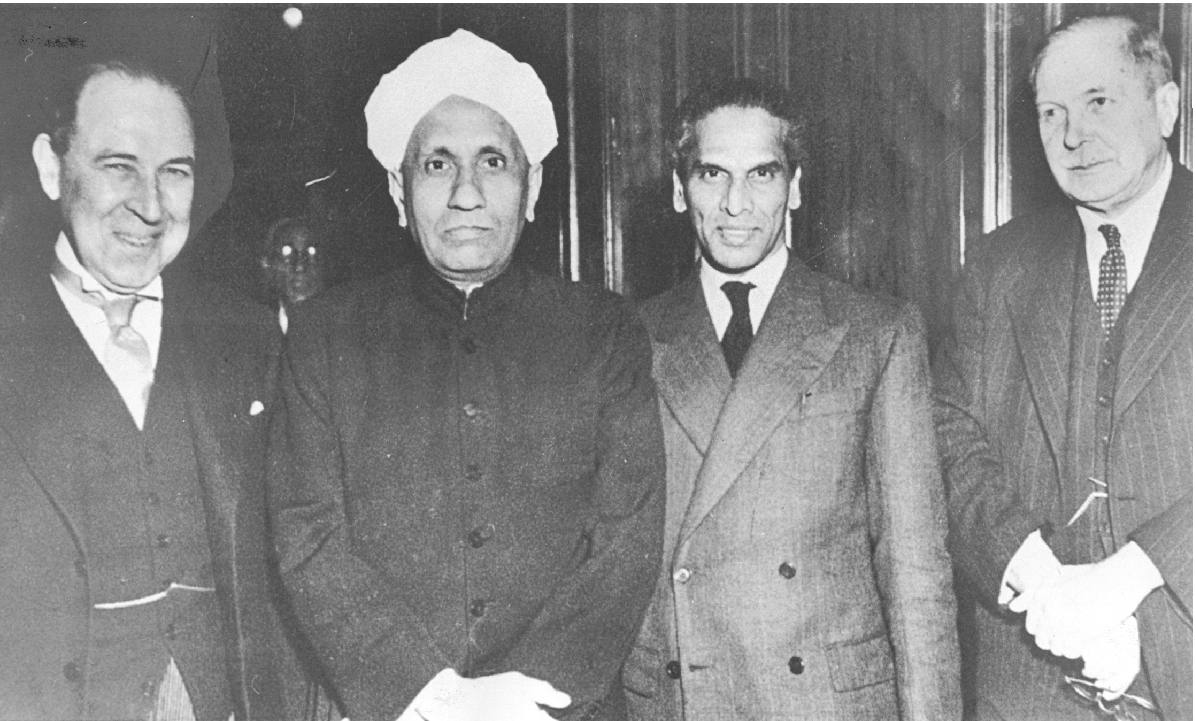
\includegraphics[scale=0.22]{"images/5.jpg"}
\caption{ಸರ್ ಜಾನ್ ಆ್ಯಂಡರ್‌ಸನ್, ಸಿ. ವಿ. ರಾಮನ್, ವಿ. ಕೆ. ಕೃಷ್ಣಮೆನನ್ ಮತ್ತು ಸರ್. ಚಾರ್ಲ್ಸ್ ಡಾರ್ವಿನ್ ಅವರು. ತಾ \enginline{11} ಮೇ \enginline{1948}ರಲ್ಲಿ ಲಂಡನ್‍ನಲ್ಲಿ ಹೈ ಕಮೀಷನರು ರಾಮನ್ ಅವರನ್ನು ಸನ್ಮಾನಿಸಿದ ಸಂದರ್ಭ (ದಿ ಹಿಂದೂ ಪತ್ರಿಕೆ)}\label{chap3-fig03}
\end{figure}


\begin{figure}[!htbp]
\centering
\includegraphics[scale=0.22]{"images/6.jpg"}
\caption{ಡಿಸೆಂಬರ್ \enginline{27}, \enginline{1951}ರಲ್ಲಿ, ಇಂಡಿಯನ್ ಅಕಾಡಮಿ ಆಫ಼್ ಸೈನ್ಸಸ್‍ನ ಹದಿನೇಳನೇ ವಾರ್ಷಿಕ ಸಭೆಯನ್ನು ರಾಷ್ಟ್ರಾಧ್ಯಕ್ಷರಾದ ರಾಜೇಂದ್ರ ಪ್ರಸಾದ ಅವರು ಉದ್ಘಾಟಿಸುತ್ತಿರುವುದು. ರಾಮನ್‍ರವರು ಎಡಗಡೆ ಕುಳಿತಿದ್ದಾರೆ (ದಿ ಹಿಂದೂ ಪತ್ರಿಕೆ)}\label{chap3-fig04}
\end{figure}

\clearpage

\begin{sidewaysfigure}[!htbp]
\centering
\includegraphics[scale=0.3]{"images/8.jpg"}
\caption{\centerline{ಲಿಂಡೋದಲ್ಲಿ ನೊಬೆಲ್ ವಿಜೇತರ ಸಮ್ಮೇಳನದಲ್ಲಿ ರಾಮನ್ \enginline{(1956)}. ವುಲ್ಫ್ ಗಾಂಗ್ ಪೌಲಿರವರು ವಿನೋದದಲ್ಲಿ ಹಾಡುತ್ತಿದ್ದಾರೆ.}  \\ \centerline{ ಮಾಕ್ಸ್ ಬಾರ್ನ್ ಚಿತ್ತಾರದ ಟೈ ಕಟ್ಟಿದ್ದಾರೆ (ದಿ ಹಿಂದು ಪತ್ರಿಕೆ)}}\label{chap3-fig05}
\end{sidewaysfigure} 

\vfill
